% Just ignore everything between this and the next commented line!

\documentclass[12pt]{article}
\usepackage[margin=1in]{geometry} 
\usepackage[usenames,dvipsnames]{xcolor}
\usepackage{amsmath,amsthm,amssymb,amsfonts, color, graphicx,ulem}
\usepackage[hidelinks]{hyperref}
\usepackage{caption}

% added by Trx, 29.11.24
\hypersetup{
    colorlinks=true,
    linkcolor=blue,
    filecolor=blue,      
    urlcolor=blue,
    citecolor=blue
}

\usepackage{datetime}
\newcommand{\N}{\mathbb{N}}
\newcommand{\Z}{\mathbb{Z}}
\newcommand{\R}{\mathbb{R}}
\newcommand{\Q}{\mathbb{Q}}
\newcommand{\PP}{\mathbb{P}}
\newcommand{\F}{\mathcal{F}}
\theoremstyle{definition}
% \newtheorem{problem}{Problem}
% \newtheorem{solution}{Solution to problem}
\newtheorem{problem}{\color{RoyalBlue}Problem}
\newtheorem{solution}{\color{ForestGreen}Solution to problem}


% Define commands for vectors
\newcommand{\va}{\mathbf{a}}
\newcommand{\vb}{\mathbf{b}}
\newcommand{\vc}{\mathbf{c}}
\newcommand{\vd}{\mathbf{d}}
\newcommand{\ve}{\mathbf{e}}
\newcommand{\vv}{\mathbf{v}}
\newcommand{\vu}{\mathbf{u}}
\newcommand{\vw}{\mathbf{w}}
\newcommand{\vx}{\mathbf{x}}
\newcommand{\vy}{\mathbf{y}}
\newcommand{\vz}{\mathbf{z}}

\usepackage{svg}
\usepackage{tikz}

\usepackage[OT6,T1]{fontenc}
\usepackage[T2A]{fontenc}
\usepackage[utf8]{inputenc}
\newcommand{\armenian}{\fontencoding{OT6}\fontfamily{cmr}\selectfont}
\DeclareTextFontCommand{\textarmenian}{\armenian}

%%%%%%%%% By Trkh+GPT for solutions
% Set up custom colors
\usepackage{mathtools}                    % For additional math formatting
\usepackage{bm}                           % For bold symbols
\usepackage{enumitem}                     % For customizable lists
\usepackage{tcolorbox}  
\usepackage{xcolor}
\definecolor{solutionbg}{rgb}{0.95, 0.95, 0.98}  % Light gray background
\definecolor{solutionborder}{rgb}{0.2, 0.2, 0.7} % Deep blue border
\usepackage{xcolor}




\begin{document}

%%%%%%%%% By Trkh+GPT for solutions

% Define a simple solution environment with colored heading
\definecolor{solutioncolor}{RGB}{34, 139, 230} % A soft blue color

\newenvironment{sol}{
    \textbf{\textcolor{solutioncolor}{\textbf{Solution:}}}
}



\title{Mathematics for Machine Learning}
% \title{Homework 1}
\author{Armenian Code Academy}
% \author{ACA, Advanced ML, Deep Learning}
% \date{Due: 24 April, 2024}
% \date{29 October, 2024}
\date{}
% Add your name in above
\maketitle
    % \input{Trx/2024_Nov_P4.tex}
    % \input{2024_Nov_pr3.tex}
    %  \begin{center}\begin{large} Practice Problems 1 \end{large}\end{center}
 \bigskip

% \documentclass{article}
% \usepackage{amsmath}

% \begin{document}

\begin{problem}
    Evaluate the expression:

    \begin{enumerate}
        \item[a) ] $3\cdot (\va + 2\vb) $,  where $\va= \begin{bmatrix} 4 \\ 5\end{bmatrix} $, $\vb= \begin{bmatrix} 2 \\ -3 \end{bmatrix} $,
        
        \item[b) ] $5\va - 10\vb $,  where $\va= \begin{bmatrix} 17 \\ 24 \end{bmatrix} $, $\vb= \begin{bmatrix} 5 \\ 12 \end{bmatrix} $,
        
        \item[c) ] $3\vu^T-(\vv+2\vw)^T$, where $\vu= \begin{bmatrix}4\\1\\-3 \end{bmatrix}, \vv= \begin{bmatrix}5\\0\\2 \end{bmatrix}, \vw= \begin{bmatrix}1\\3\\-2 \end{bmatrix}$.
    \end{enumerate}
\end{problem}

\medskip

\begin{problem}
    Michael mowed lawns on weekends to help pay his college tuition bills. He charged his customers according to the size of their lawns at a rate of \$0.5 per square foot and kept a record of the areas of their lawns in an ordered list:
$$\va = (200, 300, 50, 50, 100, 100, 200, 500, 1000, 100) .$$
He also listed the number of times he mowed each lawn in a given year. For the year 2023 that ordered list was
$$\vb = (20, 1, 2, 4, 1, 5, 2, 1, 10, 6) .$$

a) Pretend that $\va$ and $\vb$ are vectors and compute $\va  \cdot  \vb$.
\\


b) What quantity does the dot product $\va  \cdot  \vb$ measure?
\\

c) How much did Michael earn from mowing lawns in
2023? Write an expression for this amount in terms of the vectors
$\va$ and $\vb$.
\end{problem}

\newpage

\begin{problem}
    Check if the following set is a vector space:

    \begin{enumerate}
        \item [a)] $A = \Z$, with the usual operations $+$ and $\cdot$,
                
        \item [b)] $B = \left\{ \begin{bmatrix} 0 \\ 0 \\ a\end{bmatrix} \mid \text{ for all real numbers }a\in\R\right\}$ with the usual operations $+$ and $\cdot$,
        
        
        \item [c)] $C =  \R^2 = \bigg\{ \begin{bmatrix} a \\ b \end{bmatrix} \mid \text{ for all numbers }a, b\in\R\bigg\}$, with the usual operation $\cdot$ and the addition defined as:
        \[  \begin{bmatrix} x_1 \\ x_2 \end{bmatrix}  +  \begin{bmatrix} y_1 \\ y_2 \end{bmatrix}  = \begin{bmatrix} x_1+y_1 \\ x_2+y_2+1 \end{bmatrix}, \]

        
        
        \item [d)] The set of all polynomials of degree $\le 2$, with the usual operations $+$ and $\cdot$.


    \end{enumerate}

\end{problem}

\medskip


\begin{problem}
    Calculate the Manhattan (L1) and Euclidean (L2) norms of the following vectors:

    \begin{enumerate}
        \item[a) ] $\va= \begin{bmatrix} 4\\-5\\7 \end{bmatrix}$,
        
        \item[b) ] $\va+\vb$, where $\va= \begin{bmatrix}12\\5\\0\end{bmatrix}, \vb = \begin{bmatrix} -1\\2\\-2\end{bmatrix}$,
        
        \item[c) ] $13\vc$, where $\vc= \begin{bmatrix}3\\4\end{bmatrix}$,
        
        \item[d) ] $-\vd$, where $\vd= \begin{bmatrix}1\\1\\2\end{bmatrix}$.
    \end{enumerate}
\end{problem}
\bigskip


\begin{problem}
    Find the angles between the following vectors:

    \begin{enumerate}
        \item[a) ] $\va= \begin{bmatrix} 1\\3\\2\end{bmatrix}$ and $\vb= \begin{bmatrix} 4\\-4\\4\end{bmatrix}$,
        
        \item[b) ] $\va= \begin{bmatrix} 3\\0\end{bmatrix}$ and $\vb= \begin{bmatrix} 3\\3\end{bmatrix}$.
        
    \end{enumerate}
\end{problem}
\newpage

\begin{problem}
    Evaluate the expression:

    \begin{enumerate}
        \item[a) ] $AB$, where $A=\begin{bmatrix}
        3&2\\1&4   \end{bmatrix}$, $B=\begin{bmatrix}
        5&-1&2\\0&2&3   \end{bmatrix}$,

        \item[b) ] $B^2=BB$, where $B=\begin{bmatrix}
        4&-3&2\\3&-2&0\\1&1&3   \end{bmatrix}$,
        
        \item[c) ] $(A-B)C$, where $A=\begin{bmatrix}
        2&5&4\\-3&-2&4\\5&9&2   \end{bmatrix}$, $B=\begin{bmatrix}
        2&1&5\\-5&2&2\\1&6&-1   \end{bmatrix}$, $C=\begin{bmatrix}
        4&-1\\1&2\\3&3   \end{bmatrix}$.
    \end{enumerate}
\end{problem}
\bigskip



%%%%% Stexic nerqev tanel hajord practicein


    %  \begin{center}\begin{large} Homework Problems 1 \end{large}\end{center}
 \bigskip

% \documentclass{article}
% \usepackage{amsmath}

% \begin{document}


\begin{problem}%[1 point]
    Add the following vectors:

    \begin{enumerate}
        \item[a) ] $\va+\vb$, where $\va= \begin{bmatrix} 3 \\ -1 \\ 2 \end{bmatrix}, \vb=\begin{bmatrix} 2 \\ 4 \\ -5 \end{bmatrix}$,
        
        \item[b) ] $\vv^T+\vu^T+\vw^T$, where $\vv= \begin{bmatrix} 1 \\ -2 \\ 0 \end{bmatrix}, \vu = \begin{bmatrix} -3 \\ 5 \\ 2.5 \end{bmatrix}, \vw= \begin{bmatrix} -2 \\ 3 \\ 2 \end{bmatrix}$. 
    \end{enumerate}
\end{problem}

\begin{sol} 
    \subsubsection*{Part (a)}

    \[
    \va + \vb = \begin{bmatrix} 3+2 \\ -1+4 \\ 2+(-5) \end{bmatrix} = \textcolor{orange}{\begin{bmatrix} 5 \\ 3 \\ -3 \end{bmatrix}}
    \]
    
    \subsubsection*{Part (b)}
    
    \[
    \vv^T + \vu^T + \vw^T = \begin{bmatrix} 1 & -2 & 0 \end{bmatrix} + \begin{bmatrix} -3 & 5 & 2.5 \end{bmatrix} + \begin{bmatrix} -2 & 3 & 2 \end{bmatrix}
    \]
    \[
    = \begin{bmatrix} 1+(-3)+(-2) & -2+5+3 & 0+2.5+2 \end{bmatrix} = \textcolor{orange}{\begin{bmatrix} -4 & 6 & 4.5 \end{bmatrix}}
    \]
\end{sol}


\begin{problem}%[1 point]
    Multiply the following vectors and scalars:

    \begin{enumerate}
        \item[a) ] $2 \cdot \vu$,  where $\vu= \begin{bmatrix} 3 \\ -1 \\ 2 \end{bmatrix} $,
        
        \item[b) ] $ \vy \cdot (-3.2)$, where $\vy = \begin{bmatrix} 1 \\ -2 \\ 0 \end{bmatrix}$,
        
        \item[c) ] $0 \cdot \vz$, where $\vz = \begin{bmatrix}4 \\ 0 \\ -7 \end{bmatrix}$.
    \end{enumerate}
\end{problem}

\begin{sol}
    \subsubsection*{Part (a)}
    \[
    2 \cdot \vu = 2 \cdot \begin{bmatrix} 3 \\ -1 \\ 2 \end{bmatrix} = \begin{bmatrix} 2 \cdot 3 \\ 2 \cdot (-1) \\ 2 \cdot 2 \end{bmatrix} = \textcolor{orange}{\begin{bmatrix} 6 \\ -2 \\ 4 \end{bmatrix}}
    \]
    
    \subsubsection*{Part (b)}
    \[
    \vy \cdot (-3.2) = (-3.2) \cdot \begin{bmatrix} 1 \\ -2 \\ 0 \end{bmatrix} = \begin{bmatrix} -3.2 \cdot 1 \\ -3.2 \cdot (-2) \\ -3.2 \cdot 0 \end{bmatrix} = \textcolor{orange}{\begin{bmatrix} -3.2 \\ 6.4 \\ 0 \end{bmatrix}}
    \]
    
    \subsubsection*{Part (c)}
    \[
    0 \cdot \vz = 0 \cdot \begin{bmatrix} 4 \\ 0 \\ -7 \end{bmatrix} = \begin{bmatrix} 0 \cdot 4 \\ 0 \cdot 0 \\ 0 \cdot (-7) \end{bmatrix} = \textcolor{orange}{\begin{bmatrix} 0 \\ 0 \\ 0 \end{bmatrix}}
    \]
\end{sol}

%%%%%%%%%%%%%%%%%%%%%% 3 %%%%%%%%%%%%%%%%%%
\begin{problem}%[2 points]
    Calculate the dot product:
    
a) $\vu \cdot \vv$, where $\vu=\begin{bmatrix}3\\-1\\2 \end{bmatrix}$, $\vv=\begin{bmatrix}2\\4\\-5 \end{bmatrix}$,
\medskip

b) $\vx \cdot \vy$, where $\vx =\begin{bmatrix}2\\7\\3 \end{bmatrix}$, $\vy =-\vx$.
\end{problem}

\begin{sol}
        \subsubsection*{Part (a)}
    \[
    \vu \cdot \vv = \begin{bmatrix} 3 \\ -1 \\ 2 \end{bmatrix} \cdot \begin{bmatrix} 2 \\ 4 \\ -5 \end{bmatrix} = 3 \cdot 2 + (-1) \cdot 4 + 2 \cdot (-5)
    \]
    \[
    = 6 - 4 - 10 = \textcolor{orange}{-8}
    \]
    
    \subsubsection*{Part (b)}
    \[
    \vx \cdot \vy = \vx \cdot (-\vx) = -(\vx \cdot \vx)
    \]
    \[
    \vx \cdot \vx = \begin{bmatrix} 2 \\ 7 \\ 3 \end{bmatrix} \cdot \begin{bmatrix} 2 \\ 7 \\ 3 \end{bmatrix} = 2 \cdot 2 + 7 \cdot 7 + 3 \cdot 3
    \]
    \[
    = 4 + 49 + 9 = 62
    \]
    \[
    \vx \cdot \vy = -62 = \textcolor{orange}{-62}
    \]
\end{sol}



\newpage
\begin{problem}%[3 points]
    Given the vectors $\mathbf{u} = \begin{bmatrix} 4 \\ -1 \\ 6 \end{bmatrix}$ and $\mathbf{v} = \begin{bmatrix} 5 \\ 1 \\ 2 \end{bmatrix}$, calculate:
        \begin{enumerate}
            \item[a) ] $\vu+\vv$
            \item[b) ] $3\vu-2\vv$
            \item[c) ] $\vu \cdot \vv$
            \item[d) ] $(3\vv - 6\vu) \cdot \vv$
            \item[e) ] $\vv \cdot (4\vv^T - \vu^T)^T$
        \end{enumerate}
\end{problem}

\begin{sol}
        \subsubsection*{Part (a)}
    \[
    \vu + \vv = \begin{bmatrix} 4 \\ -1 \\ 6 \end{bmatrix} + \begin{bmatrix} 5 \\ 1 \\ 2 \end{bmatrix} = \begin{bmatrix} 4+5 \\ -1+1 \\ 6+2 \end{bmatrix} = \textcolor{orange}{\begin{bmatrix} 9 \\ 0 \\ 8 \end{bmatrix}}
    \]
    
    \subsubsection*{Part (b)}
    \[
    3\vu - 2\vv = 3 \cdot \begin{bmatrix} 4 \\ -1 \\ 6 \end{bmatrix} - 2 \cdot \begin{bmatrix} 5 \\ 1 \\ 2 \end{bmatrix}
    \]
    \[
    = \begin{bmatrix} 12 \\ -3 \\ 18 \end{bmatrix} - \begin{bmatrix} 10 \\ 2 \\ 4 \end{bmatrix} = \begin{bmatrix} 12-10 \\ -3-2 \\ 18-4 \end{bmatrix} = \textcolor{orange}{\begin{bmatrix} 2 \\ -5 \\ 14 \end{bmatrix}}
    \]
    
    \subsubsection*{Part (c)}
    \[
    \vu \cdot \vv = \begin{bmatrix} 4 \\ -1 \\ 6 \end{bmatrix} \cdot \begin{bmatrix} 5 \\ 1 \\ 2 \end{bmatrix} = 4 \cdot 5 + (-1) \cdot 1 + 6 \cdot 2
    \]
    \[
    = 20 - 1 + 12 = \textcolor{orange}{31}
    \]
    
    \subsubsection*{Part (d)}
    \[
    (3\vv - 6\vu) \cdot \vv = \left(3 \cdot \begin{bmatrix} 5 \\ 1 \\ 2 \end{bmatrix} - 6 \cdot \begin{bmatrix} 4 \\ -1 \\ 6 \end{bmatrix}\right) \cdot \begin{bmatrix} 5 \\ 1 \\ 2 \end{bmatrix}
    \]
    \[
    = \left(\begin{bmatrix} 15 \\ 3 \\ 6 \end{bmatrix} - \begin{bmatrix} 24 \\ -6 \\ 36 \end{bmatrix}\right) \cdot \begin{bmatrix} 5 \\ 1 \\ 2 \end{bmatrix}
    \]
    \[
    = \begin{bmatrix} -9 \\ 9 \\ -30 \end{bmatrix} \cdot \begin{bmatrix} 5 \\ 1 \\ 2 \end{bmatrix} = -9 \cdot 5 + 9 \cdot 1 + (-30) \cdot 2
    \]
    \[
    = -45 + 9 - 60 = \textcolor{orange}{-96}
    \]
    
    \subsubsection*{Part (e)}
    \[
    \vv \cdot (4\vv^T - \vu^T)^T = \vv \cdot (4 \cdot \vv - \vu)
    \]
    \[
    = \begin{bmatrix} 5 \\ 1 \\ 2 \end{bmatrix} \cdot \left(4 \cdot \begin{bmatrix} 5 \\ 1 \\ 2 \end{bmatrix} - \begin{bmatrix} 4 \\ -1 \\ 6 \end{bmatrix}\right)
    \]
    \[
    = \begin{bmatrix} 5 \\ 1 \\ 2 \end{bmatrix} \cdot \left(\begin{bmatrix} 20 \\ 4 \\ 8 \end{bmatrix} - \begin{bmatrix} 4 \\ -1 \\ 6 \end{bmatrix}\right)
    \]
    \[
    = \begin{bmatrix} 5 \\ 1 \\ 2 \end{bmatrix} \cdot \begin{bmatrix} 16 \\ 5 \\ 2 \end{bmatrix} = 5 \cdot 16 + 1 \cdot 5 + 2 \cdot 2
    \]
    \[
    = 80 + 5 + 4 = \textcolor{orange}{89}
    \]
\end{sol}

\medskip

\begin{problem}%[1 point]
    A translation office translated $\va=[24, 17, 9, 13]$ documents from English, French, German and Russian, respectively. For each of those languages, it takes about $\vb=[5, 10, 11, 7]$ minutes to translate one page.
    
    How much time did they spend translating in total? How much did each of the translators spend on average if there are $4$ translators in the office? Write an expression for this amount in terms of the vectors $\va$ and $\vb$.
\end{problem}

\begin{sol}
    \subsubsection*{Total Time Spent}

    The total time spent translating is the dot product of the vectors \(\va\) and \(\vb\):
    \[
    \text{Total Time} = \va \cdot \vb = \begin{bmatrix} 24 \\ 17 \\ 9 \\ 13 \end{bmatrix} \cdot \begin{bmatrix} 5 \\ 10 \\ 11 \\ 7 \end{bmatrix}
    \]
    \[
    = (24 \cdot 5) + (17 \cdot 10) + (9 \cdot 11) + (13 \cdot 7)
    \]
    \[
    = 120 + 170 + 99 + 91 = \textcolor{orange}{480 \text{ minutes}}.
    \]
    
    \subsubsection*{Average Time per Translator}
    
    The average time per translator, given there are \(4\) translators, is:
    \[
    \text{Average Time} = \frac{\text{Total Time}}{4} = \frac{480}{4} = \textcolor{orange}{120 \text{ minutes}}.
    \]
    
    \subsubsection*{Expression in Terms of \(\va\) and \(\vb\)}
    
    The total time in terms of \(\va\) and \(\vb\) is:
    \[
    \text{Total Time} = \va \cdot \vb
    \]
    
    The average time per translator is:
    \[
    \text{Average Time} = \frac{\va \cdot \vb}{4}
    \]
\end{sol}


\medskip

\begin{problem}[\textbf{additional}]%[2 points]
    Show that the following set is a vector space:

    \begin{enumerate}
        \item [a)] $A = \R$,
        
        \item [b)] $B = \bigg\{ \begin{bmatrix} a \\ 0 \end{bmatrix} \mid \text{ for all numbers }a\in\R\bigg\}$,

        \item [c)] The set of all polynomials of the form $ax+b$ \\(i.e. all polynomials of degree $\le 1$). 

    \end{enumerate}
    \bigskip
    {\small \textit{Hint:} \textit{to show that a set is a vector space, check that the sum of any two elements is again in the set, and that if we multiply any element of the set with any number, the result will again be in the set. Then check that conditions 1-8 (in the lecture) hold.}}
\end{problem}
\medskip
\begin{problem}[\textbf{additional}]%[2 points]
    Show that the following set is \textit{not} a vector space:

    \begin{enumerate}
        \item [a)] $A = \N$,
        
        \item [b)] $B =  \bigg\{ \begin{bmatrix} a \\ 1 \end{bmatrix} \mid \text{ for all numbers }a\in\R\bigg\}$,
        
        \item [c)] The set of all polynomials of the form $ax+b$ where $a \ne 0$.

    \end{enumerate}
    \bigskip
    {\small \textit{Hint:} \textit{Show that if we sum two elements or multiply an element with some number, the result might not always belong to the set, or that some of the conditions 1-8 does not hold.}}
\end{problem}


        
        
    %  \begin{center}\begin{large} Homework Problems 2
 \end{large}\end{center}
 \bigskip

% \documentclass{article}
% \usepackage{amsmath}

% \begin{document}


\begin{problem}[3 points]
Check if the following set is a vector space:

    \begin{enumerate}
        \item [a)] The set of real negative numbers $A = \{x\in\R \mid x < 0\}$, with the usual operations $+$ and $\cdot$,

        \item [b)] $B = \left\{ \begin{bmatrix} a \\ b \\ c\end{bmatrix} \mid \text{ for all real numbers }a, b, c\in\R\right\}$, with the usual operation of $\cdot$, and the addition defined as:
        \[ \begin{bmatrix} a_1 \\ b_1 \\ c_1\end{bmatrix} + \begin{bmatrix} a_2 \\ b_2 \\ c_2\end{bmatrix} = \begin{bmatrix} a_1 + a_2 \\ b_1 + b_2\\ c_1 + c_2 - 1\end{bmatrix} ,\]
        
        \item [c)] $C =  \bigg\{ \begin{bmatrix} a \\ b \end{bmatrix} \mid \text{ for all numbers }a,b\in\R\bigg\}$, with the usual operation of $\cdot$, and the addition defined as:
        \[ \begin{bmatrix} a_1 \\ b_1 \end{bmatrix} +\begin{bmatrix} a_2 \\ b_2 \end{bmatrix} = \begin{bmatrix} a_1-a_2 \\ b_1-b_2 \end{bmatrix} , \]

        \item [d)] $D =  \bigg\{ \begin{bmatrix} a \\ b \end{bmatrix} \mid \text{ for all numbers }a,b\in\R\bigg\}$, with the usual operation of $\cdot$, and the addition defined as:
        \[ \begin{bmatrix} a_1 \\ b_1 \end{bmatrix} +\begin{bmatrix} a_2 \\ b_2 \end{bmatrix} = \begin{bmatrix} 0 \\ 0\end{bmatrix}  ,\]
        
        \item [e)] $E =  \bigg\{ \begin{bmatrix} a \\ b \end{bmatrix} \mid \text{ for all numbers }a,b\in\R\bigg\}$, with the usual operation of $+$, and the scalar multiplication defined as:
        \[ c \cdot \begin{bmatrix} a \\ b \end{bmatrix} = \begin{bmatrix} c \cdot ( a+b) \\ cb\end{bmatrix}  , \qquad \text{for any } c>0.\]

        \item [f)] The set of all polynomials of degree $2$, with the usual operations $+$ and $\cdot$.

        
    \end{enumerate}
\end{problem}

\bigskip
\begin{problem}[2 point]
    Calculate the Manhattan (L1) and Euclidean (L2) norms of the following vectors:

    \begin{enumerate}
        \item[a) ] $\va= \begin{bmatrix} 2\\-9\\3 \end{bmatrix}$,
        
        \item[b) ] $\va-2\vb$, where $\va= \begin{bmatrix}3\\4\\1\\0\end{bmatrix}, \vb = \begin{bmatrix}4\\5\\-2\\-1\end{bmatrix}$,
        
        \item[c) ] $-3\vc$, where $\vc= \begin{bmatrix}2\\-5\\6\end{bmatrix}$.
    \end{enumerate}
    % \bigskip

    %     \textbf{Optional, not graded}: Find the angle between $\va$ in \textit{a)} and $\vc$ in \textit{c)}.
\end{problem}
\bigskip



\begin{problem}[1 point]
    Find the angles between the following vectors:

    \begin{enumerate}
        \item[a) ] $\va= \begin{bmatrix} 2\\1\\1\end{bmatrix}$ and $\vb= \begin{bmatrix} 1\\-3\\3\end{bmatrix}$,
        
        \item[b) ] The vectors $\va$ and $\vc$ in Problem 2a and 2c.

    \end{enumerate}
\end{problem}
\bigskip




% \begin{problem}[1 point]
%     Given the following system of equations, find values for $a$ and $b$:
%    \[ \begin{cases}
%          a + 3b = 4 \\
%          a - b = -4 
%     \end{cases}\]

%     How can we write the equations in terms of matrices?
% \end{problem}



\begin{problem}[2 points]
    Evaluate the expression:

    \begin{enumerate}
        \item[a) ] $AB$, where $A=\begin{bmatrix}
        6&5\\-2&7  \end{bmatrix}$, $B=\begin{bmatrix}
        -5&3\\1&4   \end{bmatrix}$,

        \item[b) ] $B^3$, where $B=\begin{bmatrix}
        -2&1&4\\1&2&1\\-2&-2&0   \end{bmatrix}$,

        \item[c) ] $CD$, where $C=\begin{bmatrix}
        7&2&-3\\0&2&8\\8&1&-3\\4&3&-1   \end{bmatrix}$, $D=\begin{bmatrix}
            -2&4\\8&1\\-1&5
        \end{bmatrix}$,
        
        \item[d) ] $(A-B)(A+B)$, where $A=\begin{bmatrix}
        2&2&4\\-3&-2&4\\-2&0&2   \end{bmatrix}$, $B=\begin{bmatrix}
        2&1&3\\-1&2&2\\1&4&-1   \end{bmatrix}$,
        
        \item[e) ] $A^2 - B^2$, with the same $A$ and $B$ as in \textit{d)}.
    \end{enumerate}
\end{problem}
\bigskip

\begin{problem}[2 points]
    Evaluate the expression:

    \begin{enumerate}
        \item[a) ] $\det(A)$, where $A=\begin{bmatrix}
        8&3&5\\1&4&2\\-4&0&4   \end{bmatrix}$,

        \item[b) ] $\text{det}(B)-\text{tr}(B)$, where $B=\begin{bmatrix}
        5&2&1\\4&-1&4\\-3&1&2 \end{bmatrix}$,
        
        \item[c) ] $\text{det}(C)$, where $C=\begin{bmatrix}
        3&0&1&3\\2&0&4&1\\0&2&-1&3\\5&0&0&3   \end{bmatrix}$,
        
        \item[d) ] $\text{det}(D)$, where $D=\begin{bmatrix}
        5&2&-3&2\\1&0&4&1\\0&5&0&-2\\1&1&5&-1  \end{bmatrix}$.
    \end{enumerate}
\end{problem}


% \bigskip

% \begin{problem}[1 point]
%     Find the value of $a$ for which the following matrices are invertible and find the inverses:
    
%     \begin{enumerate}
%         \item[a) ] $A=\begin{bmatrix}
%         8&3&5\\1&4&2\\-4&0&4   \end{bmatrix}$,

%         \item[b) ] $\text{det}(B)-\text{tr}(B)$, where $B=\begin{bmatrix}
%         5&2&1\\4&-1&4\\-3&1&2 \end{bmatrix}$,
        
%         \item[c) ] $\text{det}(C)$, where $C=\begin{bmatrix}
%         3&0&1&3\\2&0&4&1\\0&2&-1&3\\5&0&0&3   \end{bmatrix}$,
        
%         \item[d) ] $\text{det}(D)$, where $D=\begin{bmatrix}
%         5&2&-3&2\\1&0&4&1\\0&5&0&-2\\1&1&5&-1  \end{bmatrix}$.
%     \end{enumerate}
% \end{problem}


    %  \begin{center}\begin{large} Practice Problems 2
 \end{large}\end{center}
 \bigskip

% \documentclass{article}
% \usepackage{amsmath}

% \begin{document}


% \begin{problem}
%     Find the trace and determinant of the following matrices:

%     \begin{enumerate}
%         \item[a) ] $A=\begin{bmatrix}
%         2&-1\\-2&-5   \end{bmatrix}$,
        
%         \item[b) ] $B=\begin{bmatrix}
%         4&10\\34&0   \end{bmatrix}$,
        
%         \item[c) ]  $C=\begin{bmatrix}
%         2&6&3\\9&-1&4\\1&5&-2   \end{bmatrix}$,

        
%         \item[d) ]  $D=\begin{bmatrix}
%         5&-1&2\\3&1&-1\\-1&-1&-1   \end{bmatrix}$,
        
%         \item[e) ] $E=\begin{bmatrix}
%         2&0&2&4\\2&0&2&5\\2&0&2&6\\-2&0&-2&-7  \end{bmatrix}$.
%     \end{enumerate}
% \end{problem}
% \bigskip

% \begin{problem}
%     Find the inverse matrix:
%     \begin{enumerate}
%         \item[a) ] $A=\begin{bmatrix}
%         4&3\\5&-1   \end{bmatrix}$,

%         \item[b) ] $B=\begin{bmatrix}
%         7&10\\-3&2   \end{bmatrix}$.
%     \end{enumerate}
% \end{problem}
% \bigskip
% % % \bigskip
% % \newpage

% \begin{center}
%      \begin{large}
%          Solutions
%      \end{large}
%  \end{center}

%  \bigskip



%  \begin{solution} b)

%      \[ 5\va - 10\vb = 5\cdot (\va-2\vb) = 5\cdot \bigg( \begin{bmatrix} 17 \\ 24 \end{bmatrix}-2\cdot\begin{bmatrix} 5 \\ 12 \end{bmatrix} \bigg) =5\cdot \begin{bmatrix} 17-2\cdot 5 \\ 24-2\cdot 12 \end{bmatrix}=5\cdot \begin{bmatrix} 7 \\ 0 \end{bmatrix} =\begin{bmatrix} 35 \\ 0 \end{bmatrix} \]
%  \end{solution}

% \begin{solution} b)
%      \[ \vx \cdot \vy = -(\vx\cdot\vx) = -(2\cdot2+7\cdot 7 + 3\cdot 3) = -62 \]
%  \end{solution}

% \begin{solution}
%  b) $ \va \cdot \vb$ shows the area of lawn mowed by Michael, in square feet,

% c) $0.5 \va \cdot \vb.$
% \end{solution}

% \begin{solution} 
% \begin{enumerate}
%      \item[a) ]  $A = \Z$ is not a vector space; for example, $1 \in B$ but for the scalar $c=0.2$, $c \cdot 1 = 0.2 \not\in B$,
%      \item[b) ]  $B$ is a vector space (check the axioms),
%      \item[c) ]  $C$ is not a vector space, as the axiom 7 does not hold:
%  \[ c\cdot\bigg( \begin{bmatrix} x_1 \\ x_2\end{bmatrix} +  \begin{bmatrix} y_1 \\ y_2\end{bmatrix}\bigg) \neq c \cdot  \begin{bmatrix} x_1 \\ x_2\end{bmatrix}  + c \cdot  \begin{bmatrix} y_1 \\ y_2\end{bmatrix}.  \]
%      \item[d) ]  $D$ is a vector space (check the axioms).
%  \end{enumerate}

%  \end{solution}

% % % 4
%  \begin{solution} b)

%      \[ \va+\vb = \begin{bmatrix} 12-1 \\ 5+2 \\ 0-2 \end{bmatrix} = \begin{bmatrix} 11\\ 7 \\ -2 \end{bmatrix} \]
%  \[ \|\va+\vb\|_1 = |11|+|7|+|-2|=11+7+2=20  \]
%  \[ \|\va+\vb\|_2 = \sqrt{11^2+7^2+(-2)^2}=\sqrt{174}  \]

%  c)

%     \[ \|\vc\|_1 = |3|+|4|=7  \]
%     \[ \|13\vc\|_1 = 13\cdot \|\vc\|_1 = 13\cdot7=91  \]
%     \smallskip
%     \[ \|\vc\|_2 = \sqrt{3^2+4^2}=5  \]
%     \[ \|13\vc\|_2 = 13\cdot \|\vc\|_2 = 13\cdot 5=65  \]
%  \end{solution}
%  \medskip
%  \begin{solution} b) Let $\alpha$ be the angle between $\va$ and $\vb$. Then,

%  \[\cos{\alpha} = \frac{\va\cdot \vb}{\|\va\|\cdot\|\vb\|} = \frac{3 \cdot 3 + 3 \cdot 0}{\sqrt{3^2 + 0^2}\cdot \sqrt{3^2 + 3^2}} = \frac{9}{3\cdot 3\sqrt{2}} = \frac{1}{ \sqrt{2}} \]

%  \[\alpha = \arccos\frac{1}{ \sqrt{2}} = 45^{\circ}.\]
%  \end{solution}
%  \begin{solution} c) 

%  \[A - B = \begin{bmatrix}
%          2-2&5-1&4-5\\-3-(-5)&-2-2&4-2\\5-1&9-6&2-(-1)   \end{bmatrix}
%          = \begin{bmatrix}
%          0&4&-1\\2&-4&2\\4&3&3   \end{bmatrix}
%          \]

%  \begin{align*}
%      (A-&B)C=\begin{bmatrix}
%          0&4&-1\\2&-4&2\\4&3&3   \end{bmatrix} \begin{bmatrix}
%          4&-1\\1&2\\3&3   \end{bmatrix} \\&= \begin{bmatrix}
%          (0 \cdot 4 + 4 \cdot1+(-1) \cdot3) &  (0  \cdot (-1) + 4  \cdot 2 + (-1)  \cdot 3 \\
%          (2 \cdot 4 + (-4) \cdot1+2 \cdot3) &  (2  \cdot (-1) + (-4)  \cdot 2 + 2  \cdot 3 \\
%             (4 \cdot 4 + 3 \cdot1+3 \cdot3) &  (4 \cdot (-1) + 3  \cdot 2 + 3  \cdot 3 \end{bmatrix}
%             = \begin{bmatrix}
%          1&  5\\
%          10& -4 \\
%             28& 11\end{bmatrix}
%  \end{align*}
        
%  \end{solution}
%  \medskip
%  \begin{solution} a)

%  \[\text{tr}(A)=\text{tr}\bigg(\begin{bmatrix}
%          7&-1&5\\6&8&0\\10&2&-6   \end{bmatrix}\bigg) = 7+8+(-6)=9\]

%      b)

%  \[\text{det}(A)=\begin{vmatrix} 7&4\\-3&-4  \end{vmatrix}=7\cdot (-4) - 4\cdot(-3)=-28+12=-16\]


%      d) Using the cofactor method on the 4th column,

%  \begin{align*}
%      \text{det}(A)=\begin{vmatrix} 7&2&4&0\\1&5&0&0\\4&2&0&1\\-2&3&1&2  \end{vmatrix}&=0\cdot (-1)^{1+4}\cdot\begin{vmatrix} 1&5&0\\4&2&0\\-2&3&1  \end{vmatrix}  + 0\cdot (-1)^{2+4}\cdot\begin{vmatrix} 7&2&4\\4&2&0\\-2&3&1 \end{vmatrix}\\&  + 1\cdot (-1)^{3+4}\cdot\begin{vmatrix} 7&2&4\\1&5&0\\-2&3&1 \end{vmatrix} + 2\cdot (-1)^{4+4}\cdot\begin{vmatrix} 7&2&4\\1&5&0\\4&2&0 \end{vmatrix}\\&=-\begin{vmatrix} 7&2&4\\1&5&0\\-2&3&1 \end{vmatrix} +2\cdot\begin{vmatrix} 7&2&4\\1&5&0\\4&2&0 \end{vmatrix}\\&=-85+2\cdot(-72)=-229
%  \end{align*}

%      e) $\det(AB)=\det(A) \cdot \det(B) = \det(A) \cdot 0 = 0.$

%  \end{solution}

%  \begin{solution}
%      b)
%      \[ \det(A) = \begin{vmatrix}
%          7&10\\-3&2
%      \end{vmatrix} = 7\cdot 2 - 10\cdot(-3) = 14 + 30 = 44 \ne 0 \]
%      Therefore, $A$ is invertible and
%      \[ A^{-1} = \frac{1}{44}\begin{bmatrix}
%          2&-10\\3&7
%      \end{bmatrix} \]
%  \end{solution}


\begin{problem}%[2 points]
    Bring the following matrices to the Row Echelon Form and find their ranks:

    \begin{enumerate}
        \item[a) ] $A=\begin{bmatrix}6&2\\1&3\\5&2\end{bmatrix}$,
        
        \item[b) ] $B=\begin{bmatrix}4&1&2\\-4&2&-1\\8&-1&7\end{bmatrix}$,
        
        \item[c) ] $C=\begin{bmatrix}3&-2&1\\6&-4&4\end{bmatrix}$.

        \item[d) ] $D=\begin{bmatrix}2&1&4&9\\3&2&4&1\\0&1&-4&2\\-4&-1&-12&-16\end{bmatrix}$,
        
    \end{enumerate}
\end{problem}

\bigskip


\begin{problem}
    Check whether the vectors $\vv_1, \vv_2, \vv_3$ are linearly independent if:

    \begin{enumerate}
        \item[a) ] $\vv_1=\begin{bmatrix}
            1 \\ 4 \\ 2
        \end{bmatrix}, \vv_2=\begin{bmatrix}
            3 \\ 5 \\ 1
        \end{bmatrix}, \vv_3=\begin{bmatrix}
            1 \\ -3 \\ -3
        \end{bmatrix}, 
        $
        
        \item[b) ] $\vv_1=\begin{bmatrix}
            2 \\ 1 \\ -2
        \end{bmatrix}, \vv_2=\begin{bmatrix}
            3 \\ 2 \\ 0
        \end{bmatrix}, \vv_3=\begin{bmatrix}
            0 \\ 1 \\ 3
        \end{bmatrix}.
        $
        
    \end{enumerate}
\end{problem}

\bigskip 
% \newpage
\begin{problem}
    Solve the following systems of linear equations:

    \begin{enumerate}
        \item[a) ] $\begin{cases}
            3x-y=4\\
            2x+5y=-3
        \end{cases}$
        
        \item[b) ] $\begin{cases}
            x+y-z=4\\
            3x-y+z=2\\
            x-4z=2
        \end{cases}$
        
        \item[c) ] $\begin{cases}
            2x-y+z=5\\
            4x-3y=9\\
            2x-2y-z=4\\
        \end{cases}$
        
    \end{enumerate}
\end{problem}
\bigskip

% \begin{problem}
%     Find, if exists, the inverse of the matrix:

%     \begin{enumerate}
%         \item[a) ] $A=\begin{bmatrix}1&-1\\0&2\end{bmatrix}$,
        
%         \item[b) ] $B=\begin{bmatrix}1&-1&1\\2&3&0\\0&-2&1\end{bmatrix}$,
        
%         \item[c) ] $C=\begin{bmatrix}2&3&1\\3&3&1\\2&4&1\end{bmatrix}$,
        
%         \item[d) ] $D=\begin{bmatrix}2&-17&11\\-1&11&-7\\0&3&-2\end{bmatrix}$.
%     \end{enumerate}
% \end{problem}
% \bigskip

% \begin{problem}
%     Find the eigenvalues and eigenvectors of the following matrices:

%     \begin{enumerate}
%         \item[a) ] $A=\begin{bmatrix}
%             -5&2\\-7&4
%         \end{bmatrix}$,
        
%         \item[b) ] $B=\begin{bmatrix}
%             1&0\\0&1
%         \end{bmatrix}$,
        
        
%         \item[c) ] $C=\begin{bmatrix}
%             2&2&-2\\1&3&-1\\-1&1&1
%         \end{bmatrix}$,
%     \end{enumerate}

%     What are the algebraic and geometric multiplicities of the found eigenvalues?
% \end{problem}

% % \bigskip


 \newpage



\begin{solution}
    c) $C=\begin{bmatrix}
3 & -2 & 1 \\
6 & -4 & 4
    \end{bmatrix}$,
    \[
    \begin{bmatrix}
3 & -2 & 1 \\
6 & -4 & 4
    \end{bmatrix}
\xrightarrow{R_2 -2 R_1}
    \begin{bmatrix}
3 & -2 & 1 \\
0 & 0 & 2
    \end{bmatrix}
    \]
To bring the matrix to REF it is sufficient to only multiply the first row by $\frac{1}{3}$ and the second row by $\frac{1}{2}$, but we can already say that because there are 2 leading non-zero entries, $\text{rank}(C)=2$.

    
\end{solution}
\bigskip

\begin{solution}
b) To check if a set of vectors is linearly independent or not, we can put together those vectors as rows or columns of a matrix and find its rank. For example, 
\[B=
\begin{bmatrix}
     \vv_1^T \\ \vv_2^T \\ \vv_3^T
\end{bmatrix}
 =
 \begin{bmatrix}
     2 & 1 & -2 \\
     3 & 2 & 0 \\
     0 & 1 & 3
 \end{bmatrix}
 \xrightarrow{R_2 -1.5 R_1}
 \begin{bmatrix}
     2 & 1 & -2 \\
     0 & -0.5 & 3 \\
     0 & 1 & 3
 \end{bmatrix}
 \xrightarrow[R_3 + 2R_2]{R_1+2R_2}
 \begin{bmatrix}
     2 & 0 & 4 \\
     0 & -0.5 & 3 \\
     0 & 0 & 9
 \end{bmatrix}
 \]

 Again, multiplying each row with a corresponding number will result in 3 leading ones, therefore $\operatorname{rank}(B)=3$ which simply means that its rows, $\vv_1,\vv_2,$ and $\vv_3$, are linearly independent.

 \end{solution}
 \bigskip

 \begin{solution}
 b) Let $[\:A\:|\:\vb\:] $ be the augmented matrix
 \[ [\:A\:|\:\vb\:] = \begin{bmatrix}\

     1&1&-1&\vert&4\\
     3&-1&1&\vert&2\\
     1&0&-4&\vert&2
 \end{bmatrix} \]
 Bringing it to REF, we get:
 \[
 \begin{bmatrix}

     1&1&-1&\vert&4\\
     3&-1&1&\vert&2\\
     1&0&-4&\vert&2
 \end{bmatrix} 
 \xrightarrow{R_2-3R_3}
 \begin{bmatrix}
     1&1&-1&\vert&4\\
     0&-1&13&\vert&-4\\
     1&0&-4&\vert&2
 \end{bmatrix} 
 \xrightarrow{R_1+R_2}\]\[
 \begin{bmatrix}
     1&0&12&\vert&0\\
     0&-1&13&\vert&-4\\
     1&0&-4&\vert&2
 \end{bmatrix} 
 \xrightarrow{R_3-R_1}
 \begin{bmatrix}
     1&0&12&\vert&0\\
     0&-1&13&\vert&-4\\
     0&0&-16&\vert&2
 \end{bmatrix} 
 \xrightarrow{(-1)\cdot R_2}\]\[
 \begin{bmatrix}
     1&0&12&\vert&0\\
     0&1&-13&\vert&4\\
     0&0&-16&\vert&2
 \end{bmatrix} 
 \xrightarrow{-\frac{1}{16}\cdot _3}
 \begin{bmatrix}
     1&0&12&\vert&0\\
     0&1&-13&\vert&4\\
     0&0&1&\vert&-\frac{1}{8}
 \end{bmatrix} 
 \]
 At this point we can either write it in the form of an SLE and solve for $x,y,z$ or, equivalently, proceed to get the Reduced REF:
 \[
 \begin{bmatrix}

     1&0&12&\vert&0\\
     0&1&-13&\vert&4\\
     0&0&1&\vert&-\frac{1}{8}
 \end{bmatrix} 
 \xrightarrow{R_1-12R_3}
 \begin{bmatrix}
     1&0&0&\vert&\frac{3}{2}\\
     0&1&-13&\vert&4\\
     0&0&1&\vert&-\frac{1}{8}
 \end{bmatrix} 
 \xrightarrow{R_2+13R_3}
 \begin{bmatrix}
     1&0&0&\vert&\frac{3}{2}\\
     0&1&0&\vert&\frac{19}{8}\\
     0&0&1&\vert&-\frac{1}{8}
 \end{bmatrix} 
 \]
 whence we have: $x=\dfrac{3}{2},\: y=\dfrac{19}{8},\: z=-\dfrac{1}{8}$.
 \end{solution}

 \bigskip

 \begin{solution}
     c) \[
 \begin{bmatrix}
     2 & 3 & 1 & | & 1 & 0 & 0 \\
     3 & 3 & 1 & | & 0 & 1 & 0 \\
     2 & 4 & 1 & | & 0 & 0 & 1 \\
 \end{bmatrix} \xrightarrow{R_1\leftrightarrow R_2} \begin{bmatrix}
     3 & 3 & 1 & | & 0 & 1 & 0 \\
     2 & 3 & 1 & | & 1 & 0 & 0 \\
     2 & 4 & 1 & | & 0 & 0 & 1 \\
 \end{bmatrix} \xrightarrow{R_1- R_2}
 \begin{bmatrix}
     1 & 0 & 0 & | & -1 & 1 & 0 \\
     2 & 3 & 1 & | & 1 & 0 & 0 \\
     2 & 4 & 1 & | & 0 & 0 & 1 \\
 \end{bmatrix}
 \]
 \[
 \xrightarrow{R_3- R_2}\begin{bmatrix}
     1 & 0 & 0 & | & -1 & 1 & 0 \\
     2 & 3 & 1 & | & 1 & 0 & 0 \\
     0 & 1 & 0 & | & -1 & 0 & 1 \\
 \end{bmatrix}\xrightarrow{R_3 \leftrightarrow R_2}
 \begin{bmatrix}
     1 & 0 & 0 & | & -1 & 1 & 0 \\  
     0 & 1 & 0 & | & -1 & 0 & 1 \\
     2 & 3 & 1 & | & 1 & 0 & 0 \\
    
 \end{bmatrix}\]\[\xrightarrow{R_3 -2 R_1}
 \begin{bmatrix}
     1 & 0 & 0 & | & -1 & 1 & 0 \\  
     0 & 1 & 0 & | & -1 & 0 & 1 \\
     0 & 3 & 1 & | & 3 & -2 & 0 \\    
 \end{bmatrix}\xrightarrow{R_3 -3 R_2}
 \begin{bmatrix}
     1 & 0 & 0 & | & -1 & 1 & 0 \\  
     0 & 1 & 0 & | & -1 & 0 & 1 \\
     0 & 0 & 1 & | & 6 & -2 & -3 \\    
 \end{bmatrix}%=[\:I\:|\:A^{-1}\:]
 \]

 Thus,
 \[ C^{-1} = \begin{bmatrix} -1 & 1 & 0 \\ -1 & 0 & 1 \\ 6 &-2 & -3 \end{bmatrix} \]

 \end{solution}

 \bigskip
 \begin{solution}
     a) $A=\begin{bmatrix}
             -5&2\\-7&4
         \end{bmatrix}$,
        
        
         We write its characteristic polynomial to find the eigenvalues:
         \[  \det(A-\lambda I)=\left|\begin{array}{cc}
             -5-\lambda&2\\-7&4-\lambda
         \end{array}\right| =\lambda^2+\lambda-6=(\lambda+3)(\lambda-2)=0, \]
         hence both roots $\lambda = -3$ and $\lambda = 2$ have algebraic multiplicities of $1$.
         \begin{itemize}
             \item To find the eigenvectors $\vv=\begin{bmatrix}
             v_1\\v_2
         \end{bmatrix}\ne \textbf{0}$ corresponding to $\lambda = -3$, we let:
         \[
         A\vv=-3 \vv
         \]
         \[
         \begin{bmatrix}
             -5v_1 + 2v_2 \\ -7v_1 + 4v_2
         \end{bmatrix} = \begin{bmatrix}
             -3v_1 \\ -3v_2
         \end{bmatrix}
         \]
         whence we have $v_1=v_2$ (in fact, both equations give the same result). So the eigenvectors are:
         \[
         E_{-3} = \left\{ a \cdot \begin{bmatrix}
             1 \\ 1
         \end{bmatrix} \bigg\vert\: a\in\R \right\}
         \]

         Due to the fact that all vectors in $E_{-3}$ are multiples of only one vector $\begin{bmatrix}
             1 \\ 1
         \end{bmatrix}$, we see that $\dim(E_{-3})=1$, so $\lambda=-3$ has geometric multiplicity of $1$.

        
             \item To find the eigenvectors corresponding to $\lambda = 2$, we let:
         \[
         A\vv=2 \vv
         \]
         \[
         \begin{bmatrix}
             -5v_1 + 2v_2 \\ -7v_1 + 4v_2
         \end{bmatrix} = \begin{bmatrix}
             2v_1 \\ 2v_2
         \end{bmatrix}
         \]
         whence $v_1=\frac{2}{7}v_2$ (in fact, both equations give the same result). So the eigenvectors are:
         \[
         E_{2} = \left\{ a \cdot \begin{bmatrix}
             \frac{2}{7} \\ 1
         \end{bmatrix} \bigg\vert\: a\in\R \right\} = \left\{ a \cdot \begin{bmatrix}
             2 \\ 7
         \end{bmatrix} \bigg\vert\: a\in\R \right\}
         \]

         With the same logic, $\dim(E_{2})=1$, so $\lambda=2$ has geometric multiplicity of $1$ too.

         \end{itemize}
        
 \end{solution}
    %  \begin{center}\begin{large} Homework Problems 3\end{large}\end{center}
 \bigskip


\begin{problem}%[2 points]
    Bring the following matrices to the Row Echelon Form and find their ranks:

    \begin{enumerate}
        \item[a) ] $A=\begin{bmatrix}5&3&5\\1&2&-1\end{bmatrix}$,
        
        \item[b) ] $B=\begin{bmatrix}1&4&-2\\2&8&-4\\3&6&2\end{bmatrix}$,
        
        \item[c) ] $C=\begin{bmatrix}1&2&2&1\\3&2&4&2\\-2&-1&-1&-2\end{bmatrix}$,
        
        \item[d) ] $D=\begin{bmatrix}2&4&1&3&2\\-1&-2&1&0&5\\1&6&2&2&2\\3&6&2&5&1\end{bmatrix}$.
    \end{enumerate}
\end{problem}
 \bigskip


\begin{problem}%[2 points]
    Solve the following systems of linear equations using matrices:

    \begin{enumerate}
        \item[a) ] $\begin{cases}
            5x-3y=1\\
            2x+y=18
        \end{cases}$
        
        \item[b) ] $\begin{cases}
            x+5y-z=3\\
            y-z=4\\
            2x+y+z=-12
        \end{cases}$
        
        \item[c) ] $\begin{cases}
            x+4y+z=0\\
            x-z=0\\
            9y+7z=0
        \end{cases}$
        
        \item[d) ] $\begin{cases}
            x-y+3z=2\\
            4x+2y-z=-3\\
            -2x-4y+7z=7
        \end{cases}$
        
    \end{enumerate}
\end{problem}
\bigskip


% \begin{problem}[2 points]
%     Find, if exists, the inverse of the matrix:

%     \begin{enumerate}
%         \item[a) ] $A=\begin{bmatrix}2&4\\0&1\end{bmatrix}$,
        
%         \item[b) ] $B= \begin{bmatrix}
%             2 & 1 & 3 \\ 5 & -7 & 1 \\ 3 & 0 & -6 
%         \end{bmatrix}$,
        
%         \item[c) ] $C=\begin{bmatrix}0&1&1\\2&-1&1\\1&-1&-1\end{bmatrix}$,
        
%         \item[d) ] $D=\begin{bmatrix}-5&0&3&-1\\0&-5&3&-1\\3&3&-5&4\\-1&-1&4&-6\end{bmatrix}$,

%         \item[e) ] $E=\begin{bmatrix}2&1&4&9\\3&2&4&1\\0&1&-4&2\\-4&-1&-12&-16\end{bmatrix}$.
%     \end{enumerate}

% \end{problem}
% \bigskip

\begin{problem}%[1 point]
    Find the value of $a$ such that the following matrix is non-invertible:

        \[ \begin{bmatrix}
            -5 & 0 & a \\ 1 & -2 & 3 \\ 6 & -2 & 1 
        \end{bmatrix} \]
\end{problem}

% \bigskip

% \begin{problem}[2 points]
%     Find the eigenvalues and eigenvectors of the following matrices:

%     \begin{enumerate}
%         \item[a) ] $A=\begin{bmatrix}
%             1&2\\0&1\end{bmatrix}$,

%         \item[b) ] $B=\begin{bmatrix}
%             2&1\\1&2
%         \end{bmatrix}$,
        
%         \item[c) ] $C=\begin{bmatrix}
%             6&6&-12\\4&2&-6\\4&3&-7
%         \end{bmatrix}$,
        
%         \item[d) ] $D=\begin{bmatrix}
% -1&0&0\\0&-1&0\\0&0&3        \end{bmatrix}$.
%     \end{enumerate}

%     What are the algebraic and geometric multiplicities of the found eigenvalues?
% \end{problem}

% \bigskip

% \begin{problem}[1 point]
%     Are the following matrices positive definite?

%     \begin{enumerate}
%         \item[a) ] $A=\begin{bmatrix}
%             2&-1&0\\-1&2&-1\\0&-1&2
%         \end{bmatrix}$,

%         \item[b) ] $B=\begin{bmatrix}
%             5&1&1\\1&5&1\\1&1&-2
%         \end{bmatrix}$,

%         \item[c) ] $C=\begin{bmatrix}
%             3&1&2\\1&2&9\\2&2&0
%         \end{bmatrix}$.
%     \end{enumerate}
% \end{problem}


\bigskip

\begin{problem}%[\textbf{optional, not graded}]
    Find the dimension of the spans of the following vectors:

    \begin{enumerate}
        \item[a) ] $\vv_1=\begin{bmatrix}6\\1\\5\end{bmatrix},  \vv_2=\begin{bmatrix}
            2\\3\\2
        \end{bmatrix}$,

        
        \item[b) ] $\vv_1=\begin{bmatrix}6\\2\end{bmatrix},  \vv_2=\begin{bmatrix}
            1\\3
        \end{bmatrix},  \vv_3=\begin{bmatrix}
            5\\2
        \end{bmatrix}$,
        
        \item[c) ] $\vv_1=\begin{bmatrix}4\\1\\2\end{bmatrix},  \vv_2=\begin{bmatrix}
            -4\\2\\-1
        \end{bmatrix},  \vv_3=\begin{bmatrix}
            8\\-1\\7
        \end{bmatrix}$,
        
        \item[d) ] $\vv_1=\begin{bmatrix}3\\-2\\1\end{bmatrix},  \vv_2=\begin{bmatrix}
            6\\-4\\4
        \end{bmatrix}$.
        
    \end{enumerate}
\end{problem}

    %  \begin{center}\begin{large} Homework Problems 4
 \end{large}\end{center}
 \bigskip


\begin{problem}%[2 points]
    Find the eigenvalues and eigenvectors of the following matrices:

    \begin{enumerate}
        \item[a) ] $A=\begin{bmatrix}
            1&2\\0&1\end{bmatrix}$,

        \item[b) ] $B=\begin{bmatrix}
            2&1\\1&2
        \end{bmatrix}$,
        
        \item[c) ] $C=\begin{bmatrix}
            6&6&-12\\4&2&-6\\4&3&-7
        \end{bmatrix}$,
        
        \item[d) ] $D=\begin{bmatrix}
-1&0&0\\0&-1&0\\0&0&3        \end{bmatrix}$.
    \end{enumerate}

    % What are the algebraic and geometric multiplicities of the found eigenvalues?
\end{problem}

% \begin{problem}
%     Check if the following matrices are positive definite:

%     \begin{enumerate}
%         \item[a) ] $A=\begin{bmatrix}
%             10&5&2\\5&3&2\\2&2&3
%         \end{bmatrix}$,

%         \item[b) ] $B=\begin{bmatrix}
%             1&4&10\\-1&2&0\\7&2&1
%         \end{bmatrix}$.
%     \end{enumerate}
% \end{problem}

% \bigskip

% \begin{problem}
%    Find, if exists, the limit of the sequence, as $n\to\infty$:

%     \begin{enumerate}
%         \item[a) ] $\dfrac{1}{n^2}$,
        
%         \item[b) ] $\dfrac{3}{2n}$,
        
%         \item[c) ] $\dfrac{n^2}{2-n^3}$,
        
%         \item[d) ] $\dfrac{(n-1)(2-n^3)}{n^7}$,
        

%         \item[e) ] $(0.9)^n$,

%         \item[f) ] $2^n$,

%         \item[g) ] $\sin {\pi n}$,

%         \item[h) ] $\dfrac{\sin {\pi n}}{n^2}$.

%     \end{enumerate}
%     Which of the sequences above are convergent?

% \end{problem}
% \bigskip
% \newpage
\begin{problem}
    Find, if exist, the points at which the function is discontinuous:

    \begin{enumerate}
     \item[a) ] $f(x) = \begin{cases} x - 2, &  x \leq 0 \\ 2, &  x > 0 \end{cases}$
\\
     \smallskip
     \includesvg[ width=0.31\textwidth, keepaspectratio]{figs/2a}
     \smallskip
        
     \item[b) ] $f(x) = \begin{cases} x + 2, &  x > 0  \\ -\frac{1}{2}x^{2}+2, &  x \le 0 \end{cases}$
  \\
  \smallskip
     \includesvg[ width=0.31\textwidth, keepaspectratio]{figs/2b}
     \smallskip
        
        
        \item[c) ] $f(x) = \begin{cases} x + 2, &  x > 0 \\ -5, &  x = 0 \\ -\frac{1}{2}x^{2}+2, &  x < 0 \end{cases}$
  \\
  \smallskip
     \includesvg[ width=0.31\textwidth, keepaspectratio]{figs/2c}
     % \newpage
        
        
  %       \item[d) ] $f(x) = \begin{cases} \ln(x+2), &  x \leq 1, x \neq -1 \\ -1, &  x = -1 \\ -1, &  x > 1 \end{cases}$
  % \\
  % \smallskip
  %    \includesvg[ width=0.31\textwidth, keepaspectratio]{figs/2d}
        
        
    \end{enumerate}
\end{problem}
\bigskip
\begin{problem}
    Write the Taylor polynomial for the function $e^{x^2}$, around the point $x=0$.
\end{problem}
% \begin{problem}
%     For which values of $x$ is the function continuous?

%     \begin{enumerate}
%         \item[a) ] $f(x) = \dfrac{2}{x^{2} + 1}$,
        
%         \item[b) ] $g(x) = \dfrac{2x+1}{x^{2}+x-2}$,
        
%         \item[c) ] $h(x) = \begin{cases} \dfrac{x^{2} - 1}{x-1}, &  x\neq 1\\
% 2, &  x = 1 \end{cases}$
%         \end{enumerate}
% \end{problem}
% \bigskip

% TRKH-info: maybe use this for gorcnakan

% \begin{problem}
% Find the values of  
% $a$
%   that make the function  
% $f
% (
% x
% )
% $  continuous for all real numbers:

% \begin{equation*}
% f(x) = \left\{ \begin{array}{rl} 4x+5, &  \mbox{if \(x\geq -2\),} \\ x^2+a, &  \mbox{if \(x < -2\).} \end{array} \right.
% \end{equation*}

% \end{problem}

\bigskip

\begin{problem}
Calculate $f'(x)$:
    \begin{enumerate}
    \item[a) ] $10000$,

        \item[b) ] $2x^2-7x+1$,
        
        \item[c) ] $2\sin x \cdot e^x$,
        
        \item[d) ] $x^2(2-x)$,
        % \newpage
        \item[e) ] $e^{3x^2}$,
        \item[f) ] $\dfrac{2x-3}{4-x^3}$,
        \item[g) ] $\ln(\ln x)$.
    \end{enumerate}
\end{problem}

\bigskip

\begin{problem}
Find the extrema of $f(x)$ on the given set:
    \begin{enumerate}
        \item[a) ] $f(x)=3-|x+4|,\: x\in\R$,
        \item[b) ] $f(x)=2x^3+18x^2+54x+50,\: x\in\R$,
        \item[c) ] $f(x) =
      \displaystyle{\frac{2x}{x^2-2x+2}},\: x\in[0,3]$,
        \item[d) ] $f(x)=\dfrac{x^2}{x-1},\: $ on its domain,
        \item[e) ] $f(x)=\sin(x^2),\: $ on its domain.
    \end{enumerate}
\end{problem}

% \bigskip
% \bigskip


% \begin{center}
%     \begin{large}
%         Solutions
%     \end{large}
% \end{center}


% \bigskip
% \begin{solution}
%     a) Calculating the determinants of all upper-left square submatrices of $A$, we have:
%     \[ \Delta_1 = 10>0, \]
%     \[ \Delta_2 = \left|\begin{array}{cc}
%          10&5  \\
%          5&3 
%     \end{array}\right|=30-25=5>0, \]
%     \[ \Delta_3 = \left|\begin{array}{ccc}
%          10&5 &2 \\
%          5&3 &2\\
%          2&2&3
%     \end{array}\right|=3>0, \]
%     therefore $A$ is positive definite: $A \succ 0$.

%     b) $B$ is not symmetric, hence it is not positive definite (neither negative or semi-definite).
% \end{solution}

% \bigskip
% \begin{solution}
% \begin{enumerate}
%     \item[a) ] 0,
%     \item[b) ] 0,
%     \item[c) ] $\lim\limits_{n\to\infty} \dfrac{1/n}{2/n^3-1} = \dfrac{0}{-1}=0$,
%     \item[d) ] 0,
%     \item[e) ] 0,
%     \item[f) ] $+\infty$,
%     \item[g) ] $\sin \pi n = 0$ for any $n\in\N$,
%     \item[h) ] 0.
% \end{enumerate}
% \end{solution}
% \smallskip


% \begin{solution}
% \begin{enumerate}
%     \item[a) ] 0,
%     \item[b) ] $f(x)$ is continuous everywhere,
%     \item[c) ] 0,
%     \item[d) ] -1 and 1.
% \end{enumerate}
% \end{solution}
% \smallskip


% \begin{solution}
% \begin{enumerate}
%     \item[a) ] $\R$ (i.e. for any value of $a$),
%     \item[b) ] $\R\setminus\{-2,1\}$,
%     \item[c) ] $\R$ (because $\dfrac{x^2-1}{x-1}=x+1$.
% \end{enumerate}
% \end{solution}
% \smallskip


% \begin{solution}
% \[ \lim\limits_{x\to -2} 4x+5 = \lim\limits_{x\to -2} x^2+a \]
% \[ -3= 4+a \]
% \[ a= 7 \]
% \end{solution}
% \smallskip


% \begin{solution}
% \begin{enumerate}
%     \item[b) ] $12x^3+\dfrac{1}{x^2}$,
%     \item[d) ] $e^x+xe^x$,
%     \item[e) ] $6xe^{3x^2}$,
%     \item[g) ] $\dfrac{1}{\ln x}\cdot \dfrac{1}{x}$.
% \end{enumerate}
% \end{solution}
% \smallskip


% \begin{solution}
% \begin{enumerate}
%     \item[d) ] $f(x)=\dfrac{x^2}{x-1}$

%     The domain of this function is $(-\infty,1)\cup(1,+\infty)$ (in other words, it's \textit{not} continuous at $x=1$), so we must look into each of those intervals \textit{separately}.

%     As $f(x)$ is continuous on $(-\infty,1)$, we can proceed finding its critical points:
%     \[  f'(x)=\dfrac{2x(x-1)-x^2}{(x-1)^2}=\dfrac{x^2-2x}{(x-1)^2} =0\]
%     The critical points are $x=0$ (the other root $x=2$ doesn't belong to the interval). Investigating the sign of $f'(x)$ between those points, we can find out the behavior (ascending/descending) of $f(x)$ in each interval:
%     \medskip
%   \begin{center}
% \begin{tikzpicture}
%   % Axis
%   \draw[-] (-2,0) -- (1,0) node[right] {};
%   \draw[dashed,->] (1,0) -- (4,0) node[right] {$x$};
%   % \draw (0,-0.2) -- (0,0.2); % y-axis
  
%   % Points
%   \foreach \x/\label in {-1/-1, 0/0, 1/1}
%     \filldraw (\x,0) circle (2pt) node[below] {$\label$};
  
%   % Arrow
%   \draw[->, thick] (-1,0.3) -- (-0.1,0.8) node[midway, above] {};
%   \draw[->, thick] (0.1,0.8) -- (0.9,0.3) node[midway, above] {};
%   % \draw[->, thick] (5.1,0.3) -- (7.9,1.3) node[midway, above] {};
%   % \draw[->, thick] (8.1,1.3) -- (7.9,1.3) node[midway, above];
% \end{tikzpicture}
%   \end{center}
%   \medskip
% Therefore, $x=0$ is a local maximum point.

% Analogously, $x=2$ is a local minimum point.

% Another possible approach would be finding the sign of $f''(x)$ at the points $x=0$ and $x=2$.


%     \item[e) ] $f(x)=\sin(x^2)$
%     \[  f'(x)=2x\cos(x^2) =0 \]
%     The critical points are $x=0$ and all real numbers of the form $\sqrt{\frac{\pi}{2}+\pi k}$ (where $\cos(x^2)=0$), $k=1,2,\dots$. Investigating the sign of $f'(x)$ between those points, we can find out the behavior (ascending/descending) of $f(x)$ in each interval:
%     \medskip
%   \begin{center}
% \begin{tikzpicture}
%   % Axis
%   \draw[->] (-1,0) -- (9,0) node[right] {$x$};
%   % \draw (0,-0.2) -- (0,0.2); % y-axis
  
%   % Points
%   \foreach \x/\label in {0/0, 2/\dfrac{\pi}{2},5/\dfrac{\pi}{2}+\pi,8/\dfrac{\pi}{2}+2\pi}
%     \filldraw (\x,0) circle (2pt) node[below] {$\label$};
  
%   % Arrow
%   \draw[->, thick] (0,0.3) -- (1.9,1.3) node[midway, above] {};
%   \draw[->, thick] (2.1,1.3) -- (4.9,0.3) node[midway, above] {};
%   \draw[->, thick] (5.1,0.3) -- (7.9,1.3) node[midway, above] {};
%   % \draw[->, thick] (8.1,1.3) -- (7.9,1.3) node[midway, above];
% \end{tikzpicture}
%   \end{center}
%   \medskip
% Therefore, $x=0$ and $x=\dfrac{\pi}{2}+\pi+2\pi k$, $k=0,1,2,\dots$ are local minimum points, while $x=\dfrac{\pi}{2}+2\pi k$ are local maximum points.
% \end{enumerate}
% \end{solution}
% \smallskip


    %  \begin{center}\begin{large} Homework Problems 4
 \end{large}\end{center}
 \bigskip

\begin{problem}[2 points]
   Find, if exists, the limit of the sequence, as $n\to\infty$:

    \begin{enumerate}
        \item[a) ] $\dfrac{3-n}{2}$,
        
        \item[b) ] $\dfrac{3-n^2}{2+n^3}$,
        
        \item[c) ] $\dfrac{(n+1)^2(n+2)^3}{n^6}$,
        
        \item[d) ] $\dfrac{(n+1)^2(n+2)^3}{n^5}$,
        
        \item[e) ] $1^n$,

        \item[f) ] $(-1)^n$,

        \item[g) ] $\left(\dfrac{1}{0.99}\right)^n$,

        \item[h) ] $\sin {n}$,

        \item[i) ] $\dfrac{\sin {n}}{n}$.

    \end{enumerate}
    Which of the sequences above are convergent?

\end{problem}

\bigskip

\begin{problem}[2 points]
Find the value of $c$, if exists, such that the following function 
$f
(
x
)$ is continuous at 
$2$.
    \begin{enumerate}
    \item[a) ] $
f(x)=\begin{cases} 3x-5,& \text{if \(x\neq 2\)} \\  x^2+c,& \text{if \(x\ge2\)} \end{cases} $

        \item[b) ] $
f(x)=\begin{cases} x^3+1,& \text{if } x<2 \\  cx^2,& \text{if \(x\ge2\)} \end{cases} $ 
        
        \item[c) ] $
f(x)=\begin{cases} -7,& \text{if } x<2 \\ c,& \text{if } x=2 \\  4+3\sin(\pi x),& \text{if \(x>2\)} \end{cases} $
\bigskip
        
        \item[d) ] $
f(x)=\begin{cases} {\dfrac{x^2-x-2}{x-2}},& \text{if \(x\neq 2\)} \\  c,& \text{if \(x<2\)} \end{cases} $
        
    \end{enumerate}
\end{problem}
\bigskip


\begin{problem}[2 points]
Find the derivatives of the following functions:
    \begin{enumerate}
    \item[a) ] $10000$,

        \item[b) ] $2x^2-7x+1$,
        
        \item[c) ] $2\sin x \cdot e^x$,
        
        \item[d) ] $e^{x^2}$,
        \item[e) ] $x^2\ln x$,
        \item[f) ] $\dfrac{x^2}{x^3}$,
        \item[g) ] $\dfrac{x^2}{x^3+1}$,
        \item[h) ] $\sin(\cos x)$.
    \end{enumerate}
\end{problem}
\bigskip


\begin{problem}[3 points]
Find the points of local extremum of $f(x)$ on the given set:
    \begin{enumerate}
    \item[a) ] $f(x)=5x-x^2,\: x\in[2,12]$,
    \item[b) ] $f(x)=3x+1, \: x\in[-5, 5]$,
    \item[c) ] $f(x)=\dfrac{x-1}{x^2+1},\: x\in\R$,
    \item[d) ] $f(x)=\dfrac{x^3}{e^x},\: x\in\R$,
        \item[e) ] $f(x)=\cos x-\sin x,\: x\in[0,\pi]$.
        
    \end{enumerate}
\end{problem}
\bigskip


\begin{problem}[1 point]
Calculate $\displaystyle \int f(x)\, dx$:
    \begin{enumerate}
        \item[a) ] $f(x)=x^3$,
        \item[b) ] $f(x)=7x^4-3$,
        \item[c) ] $f(x)=\cos4x$,
    \end{enumerate}
\end{problem}


\bigskip

\begin{problem}[\textbf{optional, not graded}]
Match the graphs 1-4 to functions i-iv: 
\\~\\
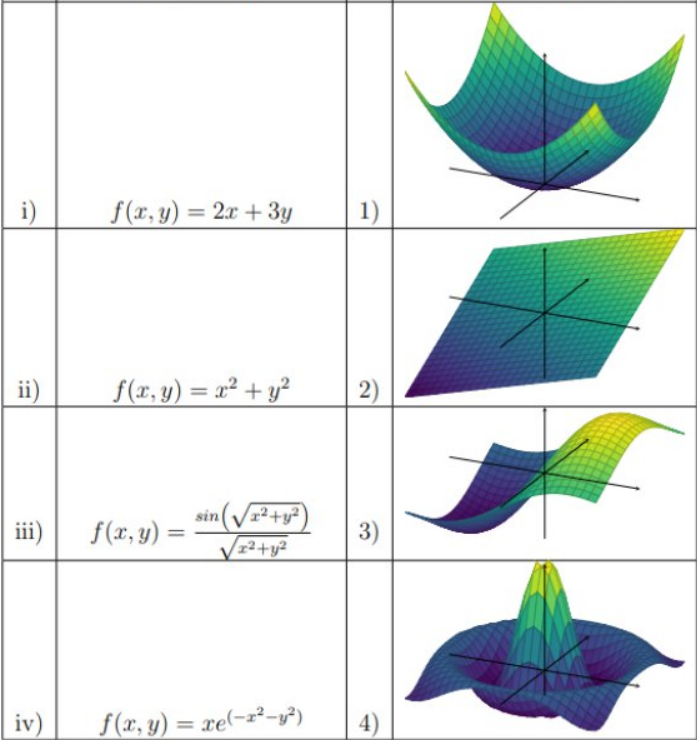
\includegraphics[width=0.7\linewidth]{figs/f(x,y) functions.png}
\\~\\
\end{problem}
    %  \begin{center}\begin{large} Practice Problems 4
 \end{large}\end{center}
 \bigskip

\begin{problem}
    Calculate $\displaystyle \int f(x)\, dx$:
    \begin{enumerate}
        \item[a) ] $f(x)=3x^2$,
        \item[b) ] $f(x)=x+6\cos x$,
        \item[c) ] $f(x)=\dfrac{3}{x}-1$,
        \item[d) ] $f(x)=\dfrac{4x}{1-2x^2}$,
        \item[e) ] $f(x)=\dfrac{2x}{1-x^2}$,
        \item[f) ] $f(x)=\text{tg}\,x$.
    \end{enumerate}
\end{problem}

\bigskip

\begin{problem}
Calculate the partial derivatives and Hessian matrices:
\begin{enumerate}
        \item[a) ] $f(x,y)=3x-2y^2$,
        \item[b) ] $f(x,y)=y^7-2x^3+x^2$,
        \item[c) ] $f(x,y)=\sin{xy}$,
        \item[d) ] $f(x,y)=x^y$,
        \item[e) ] $f(x,y)=\dfrac{x}{y}$.
    \end{enumerate}
\end{problem}

\newpage

\begin{problem}
Calculate the directional derivative:
\begin{enumerate}
        \item[a) ] $f(x, y) = x^2+y^2$ at the point $(1, 2)$ in the direction of $\dfrac{\vv}{\|\vv\|},\,\vv = (3,-4)$,
        \item[b) ] $f(x, y) = \sin(xy)$ at the point $(\pi, 0)$ in the direction of $\dfrac{\vv}{\|\vv\|},\,\vv = (1,1)$.
    \end{enumerate}
\end{problem}

\bigskip

\begin{problem}
Find, if they exist, the local extrema of $f(\vx)=f(x,y)$:
\begin{enumerate}
        \item[a) ] $f(x,y)=x^3-y$,
        \item[b) ] $f(x,y)=x^2-xy$.
    \end{enumerate}
\end{problem}
\bigskip

\begin{problem}
Suppose we roll two fair dice. What is the probability of getting
\begin{enumerate}
    \item[a) ] $2$ on each of them,
    \item[b) ] at least one $1$,
    \item[c) ] exactly one $1$,
    \item[d) ] one $1$ and one $4$,
    \item[e) ] $1$ on the first one and $4$ on the second one?
\end{enumerate}
\end{problem}
\bigskip

\begin{problem}
There are $2$ red, $5$ blue and $6$ yellow pencils in the box. We take two of them out randomly. What is the probability that both of them are
\begin{enumerate}
    \item[a) ] red,
    \item[b) ] of the same color,
    \item[c) ] of different colors,
    \item[d) ] not yellow,
    \item[e) ] not green.
\end{enumerate}
\end{problem}
\bigskip


\begin{problem}
Suppose we roll two fair dice. What is the probability of getting
\begin{enumerate}
    \item[a) ] $5$ on each of them, given that the sum of the resulting numbers is divisible by $5$.
    \item[b) ] at least one $6$, given that the sum of the two numbers is $8$.
\end{enumerate}
\end{problem}

\newpage

\begin{center}
    \begin{large}
        Solutions
    \end{large}
\end{center}


\bigskip

\begin{solution}
\begin{enumerate}
    \item[e) ] $\displaystyle \int \dfrac{2x}{1-x^2} \, dx = \int \dfrac{(x^2)'}{1-x^2} \, dx = \int \dfrac{1}{1-x^2} \, d(x^2) = \int \dfrac{1}{1-y} \, dy=-\ln|1-y|+C=-\ln|1-x^2|+C$,
    \item[f) ] $\displaystyle \int \text{tg}{x} \, dx = \int \dfrac{\sin x}{\cos x} \, dx =  - \int \dfrac{(\cos x)'}{\cos x} \, dx =  - \int \dfrac{1}{\cos x} \, d(\cos x)=  - \int \dfrac{1}{y} \, dy=  - \ln|y|+C=  - \ln|\cos x|+C$.
\end{enumerate}
\end{solution}
\smallskip



\begin{solution}
\begin{enumerate}
        \item[b) ] $f(x,y)=y^7-2x^3+x^2$,
        \begin{align*}
            & f_x(x,y) = -6x^2 + 2x, \\
            & f_y(x,y) = 7y^6, \\
            & H(x,y) = \begin{bmatrix}
                -12x+2 & 0 \\
                0 & 42y^5
            \end{bmatrix}
        \end{align*}
        
        \item[c) ] $f(x,y)=\sin{xy}$,
                \begin{align*}
            & f_x(x,y)=y\cos{xy}, \\
            & f_y(x,y)=x\cos{xy},  \\
            & H(x,y) = \begin{bmatrix}
                -y^2 \sin{xy} & \cos{xy} - xy \sin{xy} \\
                \cos{xy} - xy \sin{xy} & -x^2 \sin{xy}
            \end{bmatrix}
        \end{align*}
        
        \item[d) ] $f(x,y)=x^y$,
                        \begin{align*}
            & f_x(x,y)=yx^{y-1}, \\
            & f_y(x,y)=x^{y}\cdot \ln|x|, \\
            & H(x,y) = \begin{bmatrix}
                y(y-1)x^{y-2} & x^{y-1} + yx^{y-1}\ln|x| \\
                x^{y-1} + yx^{y-1}\ln|x| & x^y (\ln|x|)^2
            \end{bmatrix}
        \end{align*}
\end{enumerate}
\end{solution}
\smallskip


\begin{solution}
\begin{enumerate}
        \item[a) ] First let's denote by a separate variable $\vu = \dfrac{\vv}{\|\vv\|}=\begin{bmatrix}
            3/5\\-4/5
        \end{bmatrix}$. Then we calculate:
        \[ f_x(x,y) = 2x, \qquad f_x(1,2)=2, \]
        \[ f_y(x,y) = 2y, \qquad f_y(1,2)=4, \]
        so the directional derivative of $f(x,y)$ at the given point is:
        \[ \nabla_\vu f(1,2) = f_x(1,2)\cdot u_1+ f_y(1,2)\cdot u_2 = 2\cdot \dfrac{3}{5} + 4 \cdot \left(-\dfrac{4}{5}\right) = -2. \]
        
        \item[b) ] First let's denote by a separate variable $\vu = \dfrac{\vv}{\|\vv\|}=\begin{bmatrix}
            1/\sqrt{2}\\1/\sqrt{2}
        \end{bmatrix}$. Then we calculate:
        \[ f_x(x,y) = y\cos(xy), \qquad f_x(\pi,0)=0, \]
        \[ f_y(x,y) = x\cos(xy), \qquad f_y(\pi,0)=\pi, \]
        so the directional derivative of $f(x,y)$ at the given point is:
        \[ \nabla_\vu f(\pi,0) = f_x(\pi,0)\cdot u_1+ f_y(\pi,0)\cdot u_2 = \dfrac{\pi}{\sqrt{2}}. \]

        
\end{enumerate}
\end{solution}
\smallskip



\begin{solution}
\begin{enumerate}
        \item[a) ] $f(x,y)=x^3-y$
        
        The domain of this function is $(x,y)\in\R^2$. First we need to find its critical points:
\[ f_x(x,y)=3x^2, \]
\[ f_y(x,y)=-1. \]
Since $f_y(x,y)\ne 0$ for any $(x,y)$, this function has no critical points, hence no extremum point.

        
        \item[b) ] $f(x,y)=x^2-xy$
        
    The domain of this function is $(x,y)\in\R^2$. First we need to find its critical points:
\[ f_x(x,y)=2x-y=0,\]
\[ f_y(x,y)=-x=0. \]
The only critical point is $\vx = \begin{bmatrix}
    0 \\ 0
\end{bmatrix}$. In order to find whether it's an extremum or a saddle point, we need to check if its Hessian matrix is positive definite, negative definite or neither of those.
\[  f_{xx}(x,y) = 2,  \]
\[  f_{xy}(x,y)=f_{yx}(x,y) = -1,  \]
\[  f_{xx}(y,y) = 0,  \]
hence its Hessian is:
\[ H(x,y) = H(0,0) = \begin{bmatrix}2&-1\\-1&0\end{bmatrix}. \]
Finally, we check its definiteness:
\[ \Delta_1 = 2 > 0, \]
\[ \Delta_2 = \left|\begin{array}{cc}
    2 & -1 \\
    -1 & 0
\end{array}\right| =-1< 0, \]
therefore the Hessian matrix is neither positive, nor negative definite. It follows that $\vx=\begin{bmatrix}
    0\\0
\end{bmatrix}$ is a saddle point, hence this function has no extremum point.

        
\end{enumerate}
\end{solution}
\smallskip

\begin{solution}
\begin{enumerate}
    \item[a)] Assuming an equiprobable probability space $(\Omega,\F,\PP)$, let's denote the event of getting $2$ on the first die by $A$, and on the second die by $B$. Since $A$ and $B$ are independent,
\[
\PP(A \cap B) = \PP(A)\cdot\PP(B) = \dfrac{1}{6}\cdot\dfrac{1}{6} = \dfrac{1}{36}.
\]

    \item[b)] Since 
    \[
     \PP(\text{getting at least one }1) = 1 - \PP(\text{getting no }1\text{s}),
    \]
    and getting no $1$s means having $2$, $3$, $4$, $5$ or $6$ on both dice,
    \[
      \PP(\text{getting at least one }1) = 1 - \left(\dfrac{5}{6}\right)^2 = \dfrac{11}{36}.
    \]

    An alternative approach would be:
        \[
      \PP(\text{getting at least one }1) =\PP(\text{getting exactly one }1) + \PP(\text{getting two }2\text{s})  = 2\cdot\dfrac{1}{6}\cdot \dfrac{5}{6} + \dfrac{1}{6}\cdot \dfrac{1}{6} = \dfrac{11}{36}.
    \]

    
    \item[c)] $\dfrac{5}{18}$.


    \item[d)] There are two desired outcomes:
    \[
            A = \{(1, 4), (4,1)\},
    \]
    therefore the probability of getting one $1$ and one $4$ is $\dfrac{2}{36} = \dfrac{1}{18}$.
    

    \item[e)] There is only one desired outcome $(1,4)$, hence $\dfrac{1}{36}$.
    
\end{enumerate}



\end{solution}
\smallskip


\begin{solution} There are $13$ pencils in total, out of which we can select $|\Omega| = C^2_{13}=78$ pairs.
\begin{enumerate}
    \item[a)] There is only one possible way to select the only two red pencils ($|A|=C^2_2=1$), so $\PP(\text{both red})=\dfrac{1}{78}$.

    \item[b)] $
     \PP(\text{same color}) = 
        \PP({\text{both red}}) 
        + \PP({\text{both blue}})
        + \PP({\text{both yellow}})
        = \dfrac{C_{2}^2+C_{5}^2+C_{6}^2}{78} = \dfrac{1}{3},
    $
    or, if we denote the event of both pencils being red by $R$, blue by $B$ and yellow by $Y$,
    \[
        \PP(\text{same color}) = \PP(R \cup B \cup Y) = \PP(R) + \PP(B) + \PP(Y) = \dfrac{2}{13} \cdot \dfrac{1}{12}
        + \dfrac{5}{13} \cdot \dfrac{4}{12}
        + \dfrac{6}{13} \cdot \dfrac{5}{12} = \dfrac{1}{3}.
    \]
    
    \item[c)] $\PP(\text{different colors}) = 1 - \PP(\text{same color}) = 1 - \dfrac{1}{3} = \dfrac{2}{3}$.


    \item[d)] Saying that both of them are not yellow is equivalent to say each of them is either red or blue. Out of all possible outcomes we can take $C_{2+5}^2=21$ combinations without any yellow pencils, hence the probability is $\dfrac{21}{78}=\dfrac{7}{26}$.
    

    \item[e)] Zero, as none of them is green.
    
\end{enumerate}



\end{solution}
\smallskip

\begin{solution}
\begin{enumerate}
    \item[a)] Let's denote the event of getting $5$ on each of the dice by $A$, and by $B$, the event of their sum being divisible by $5$. Then,
\begin{align*}
    A &= \{(5,5)\}, \\
    B& = \{(x,y) \mid x+y = 5k\} =  \{(x,y) \mid x+y \in \{5,10\}\} \\&= \{(1, 4), (2, 3), (3, 2), (4, 1), (4, 6), (5, 5), (6,4)\}.
\end{align*}

We have:
\[
\PP(A) = \dfrac{1}{36}, \qquad \PP(B)=\dfrac{7}{36},
\]
and because $A\subset B$,
\[
\PP(A\mid B) = \dfrac{\PP(A\cap B)}{\PP(B)} = \dfrac{\PP(A)}{\PP(B)} = \dfrac{1/36}{7/36} = \dfrac{1}{7}. 
\]

    \item[b)] There are only five outcomes where the sum of the numbers equals $8$, and in only two of them one of the dice is $6$, so we get $\dfrac{2}{5}=0.4$.

    An alternative approach would be denoting the event of having at least one $6$ by $A$, and the sum being $8$ by $B$, whence
\[
 \PP(A \mid B) = \dfrac{\PP(A\cap B)}{\PP(B)} = \dfrac{2/36}{5/36} = 0.4.
\]
\end{enumerate}
\end{solution}
\smallskip

    %  \begin{center}\begin{large} Homework Problems 5
 \end{large}\end{center}
 \bigskip


\begin{problem}
    Calculate $\displaystyle \int f(x)\, dx$:
    \begin{enumerate}
        \item[a) ] $f(x)=3x^2$,
        \item[b) ] $f(x)=x+6\cos x$,
        \item[c) ] $f(x)=\dfrac{3}{x}-1$,
        \item[d) ] $f(x)=\dfrac{4x}{1-2x^2}$,
        % \item[e) ] $f(x)=\dfrac{2x}{1-x^2}$,
        \item[e) ] $f(x)=\text{tg}\,x$.
    \end{enumerate}
\end{problem}


% \bigskip

\begin{problem}%[\textbf{optional, not graded}]
Match the graphs 1-4 to functions i-iv: 
\\~\\
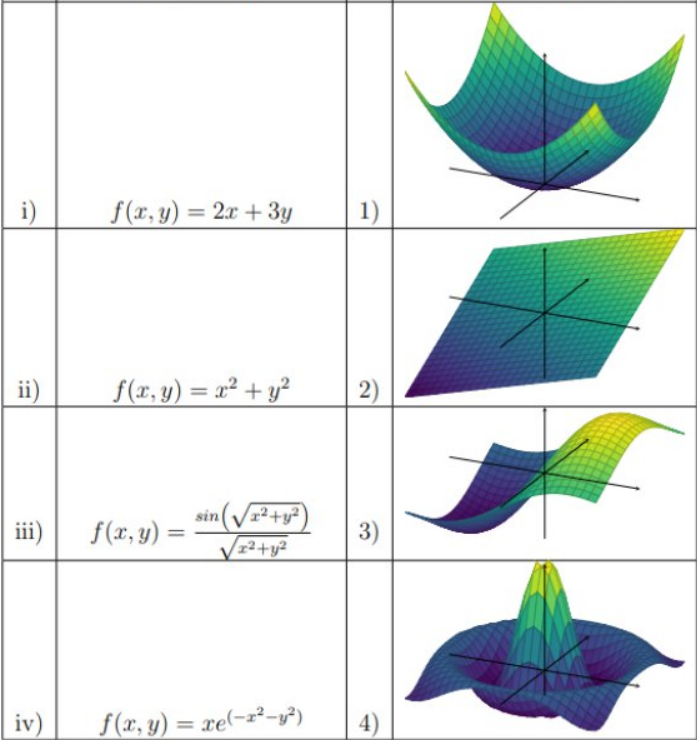
\includegraphics[width=0.6\linewidth]{figs/f(x,y) functions.png}
\\~\\
\end{problem}

% \bigskip

\begin{problem}
Calculate the partial derivatives and Hessian matrices:
\begin{enumerate}
        \item[a) ] $f(x,y)=3x-2y^2$,
        \item[b) ] $f(x,y)=y^7-2x^3+x^2$,
        \item[c) ] $f(x,y)=\sin{xy}$,
        \item[d) ] $f(x,y)=x^y+\dfrac{x}{y}$.
    \end{enumerate}
\end{problem}
\bigskip
\begin{problem}
Calculate the directional derivative:
\begin{enumerate}
        \item[a) ] $f(x, y) = (x-y)^2$ at the point $(1, 2)$ in the direction of $\dfrac{\vv}{\|\vv\|},\,\vv = (3,-4)$,
        \item[b) ] $f(x, y) = x \log y + (1-x) \log (1-y)$ at the point $(\pi, 0)$ in the direction of $\dfrac{\vv}{\|\vv\|},\,\vv = (1,1)$.
    \end{enumerate}

{\small Note: $\log x=\ln x$.}
    
\end{problem}

\bigskip


\begin{problem}
Suppose we roll two fair dice. What is the probability of getting
\begin{enumerate}
    \item[a) ] $2$ on each of them,
    \item[b) ] at least one $1$,
    \item[c) ] exactly one $1$,
    \item[d) ] one $1$ and one $4$,
    \item[e) ] $1$ on the first one and $4$ on the second one?
\end{enumerate}
\end{problem}
\bigskip

\begin{problem}
There are $2$ red, $5$ blue and $6$ yellow pencils in the box. We take two of them out randomly. What is the probability that both of them are
\begin{enumerate}
    \item[a) ] red,
    \item[b) ] of the same color,
    \item[c) ] of different colors,
    \item[d) ] not yellow,
    \item[e) ] not green.
\end{enumerate}
\end{problem}
% \bigskip

\bigskip

\begin{problem}
     \\~\\
\begin{center}
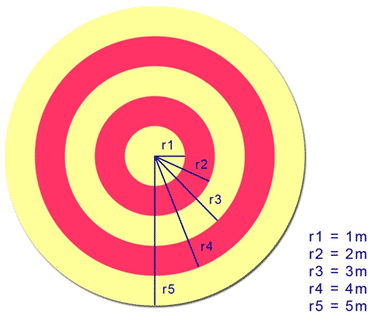
\includegraphics[width=0.5\linewidth]{figs/prob1.png}
\end{center}
\\~\\
Assume that any thrown dart will land somewhere within the circular area. The radius of circle $1$ (the inner-most yellow circle) is $1$ meter. Each radius thereafter increases by $1$ m, as shown. We throw a dart randomly. Find the probability that it lands on
\begin{enumerate}
    \item[a) ] circle $1$,
    \item[b) ] a red circle,
    \item[c) ] a yellow circle.
    
\end{enumerate}
\end{problem}
    % \input{Trx/2024_Nov_P5_Probability_continued}
    %  
 \begin{center}\begin{large} Practice Problems 5
 \end{large}\end{center}
 \bigskip

\bigskip



\begin{problem}
There are two boxes containing $\{5, 11, 8\}$ and $\{10, 8, 6\}$ white, black, red pencils respectively. One pencil is drawn from each box. What is the probability that the pencils have the same color?
\end{problem}
\bigskip


\begin{problem}
Suppose that you know the answers to 20 questions out of the total 25
questions in the entrance examination, from which you are only asked
3 random questions. What is the probability that you answer all of
the questions?
\end{problem}

\bigskip

\begin{problem}
There are two boxes containing {5, 11} and {10, 8} white, black balls
respectively. First, we take out a ball from each of the boxes. Then, we randomly choose one of them. What is the probability that the
final ball is white?
\end{problem}

\bigskip

\begin{problem}
There are three boxes having 4 white and 6 black balls in each of them.
Suppose we perform the following steps in the given order:
    \begin{enumerate}
        \item[a) ] take out a ball from the first box and put it into the second one,
        \item[b) ] take out a ball from the second box and put it into the third one,
        \item[c) ] take out a ball from the third box and put it into the first one.
    \end{enumerate}
    What is the probability of taking a white ball from the third box (after doing \textit{a)-c)})?
\end{problem}

\bigskip

\begin{problem}
Two factories produce similar weapons and deliver it to the army warehouse. The first factory’s productivity is two times more than that of
the second one. Moreover, $40\%$ of the weapons produced by the first
factory have some defects, while the same indicator is only $16\%$ for
the second factory. We randomly take a weapon from the warehouse,
test it and it appears to have no defects. What is the probability that
the weapon was produced by the first factory?

\end{problem}


\bigskip

\begin{problem}
According to some statistics, $5\%$ of all males and $0.25\%$ of all females
are color-blind. Assuming that the populations of males and females
are equal, what is the probability that a randomly chosen color-blind person is a male?
\end{problem}

\bigskip

\begin{problem}
    Nune uses her car $30\%$ of the time, walks $30\%$ of the time and rides the bus $40\%$ of the time as she goes to work. She is late $10\%$ of the time when she walks, $3\%$ of the time when she drives, and $7\%$ of the time she takes the bus.

\begin{enumerate}
    \item[a) ] What is the probability she took the bus if she was late?
    
    \item[b) ] What is the probability she walked if she is on time?
\end{enumerate}

\end{problem}

\bigskip
\begin{problem}
    On the way to the ACA, your
bus passes through a traffic light. The light cycle of the traffic light is $20$
seconds red, $5$ seconds yellow, and $50$ seconds green. What is the
probability that you will pass under a green light?
\end{problem}

\bigskip

\begin{problem}
After a trip to Garni-Geghard, you bring your camera film to a photography shop. Unfortunately, the shop ruins $4$ photos in a row from your roll which contains $24$ photos. What is the probability that the ruined photos included the
\begin{enumerate}
    \item[a) ] eighth, ninth or tenth photos,
    \item[b) ] eighth, ninth and tenth photos
\end{enumerate}
on the roll (the photos of the Garni Temple)?
\end{problem}

\bigskip

\begin{problem}
    Anush and Nairi are shopping at the mall. They agree to split up for a time and then meet for lunch. They plan to meet in
front of Kinopark between 12:00 and 13:00. The one who arrives first agrees to wait $15$ minutes for the other to arrive. After $15$
minutes, that person will leave and continue shopping. What is the probability that they will meet if each one of them arrives at any time between 12:00 and 13:00?

\textit{Hint: Try to represent the problem on coordinate system, by letting
$x$ denote the time Anush arrives, and $y$, the time Nairi arrives.}
\end{problem}

\bigskip

\begin{problem}
    A line segment is $8$ cm long. Two points are put on the segment at
random locations. What is the probability that the three segments formed by
the two points can make a triangle?
\end{problem}


\bigskip

\begin{problem}
 Vahe added a dot on the   
\includegraphics[height=0.9em]{figs/4.png} side of the die, making it 
\includegraphics[height=0.9em]{figs/5.png}, and then added two dots on the 
\includegraphics[height=0.9em]{figs/1.png} side, making it 
\includegraphics[height=0.9em]{figs/3.png}.
   What is the probability that the outcome of the die is greater than $4$? Find the expectation and variance of the die.
   
\end{problem}


\bigskip

\begin{problem}
   Let $X$ be a random variable with the PDF:
   \[
   f(x) = \begin{cases}
       2x, & 0 \le x \le 1 \\
       0, & \text{otherwise}
   \end{cases}
   \]

   Find the expectation and variance of
   \begin{enumerate}
       \item[a) ] $X$,
       \item[b) ] $2X$,
       \item[c) ] $2X + 7$. 
       
   \end{enumerate}
\end{problem}









% \newpage


% \begin{center}
%     \begin{large}
%         Solutions
%     \end{large}
% \end{center}

% \bigskip


% \begin{solution}
% Let's denote the event of drawing a white, black, red ball from the first box by $W_1$, $B_1$, $R_1$, respectively; and $W_2$, $B_2$, $R_2$ for the second box. Then the event of having two balls of the same color is equivalent to either having two whites, or two blacks, two reds. Therefore,
% \begin{align*}
%     \PP\big((W_1\cap W_2) &\text{ or } (B_1\cap B_2) \text{ or } (R_1\cap R_2) \big) \\&= \PP\big(W_1\cap W_2)+\PP(B_1\cap B_2) +\PP(R_1\cap R_2) \\&= \PP\big(W_1)\PP(W_2)+\PP(B_1)\PP(B_2) +\PP(R_1) \PP(R_2) \\&= \dfrac{5}{24}\cdot \dfrac{10}{24} +  \dfrac{11}{24}\cdot \dfrac{8}{24} +  \dfrac{8}{24}\cdot \dfrac{6}{24} = \dfrac{186}{576} = \dfrac{31}{96} 
% \end{align*}

% An alternative approach would be counting all $24\times 24$ pairs and calculating the probability of one-colored pairs.
% \end{solution}
% \smallskip




% \begin{solution}
% For us to answer all 3 questions correctly, they have to be from the 20 questions we have learned. Let $Q_1, Q_2, Q_3$ be the events of the first, second, third questions being from the questions we know. Then
% \[\PP(Q_1 \cap Q_2 \cap Q_3) = \PP(Q_1)\cdot \PP(Q_2\mid Q_1)\cdot \PP(Q_3 \mid Q_1, Q_2) = \dfrac{20}{25}\dfrac{19}{24}\dfrac{18}{23} = \dfrac{57}{115}. \]

% Or we can just calculate the number of all possible triplets: $C_{25}^{3}$, the number of triplets from questions we know: $C_{20}^{3}$, and divide the latter one by the former:
% \[
% \dfrac{C_{20}^{3}}{C_{25}^{3}} = \dfrac{57}{115}.
% \]
% \end{solution}
% \smallskip


% % \begin{solution}
% % Let's denote the number of unique (distinct) colors of the 3 balls drawn by $X$. ($X$ is a random variable.)

% % Then
% % \[\PP(X\ge 2) = 1 - \PP(X<2) = 1-\PP(X=1),\]
% % so its easier to calculate $\PP(X=1)$ (i.e. the probability that all 3 are of the same color), and subtract it from $1$. The same way as we calculated above, we can see that:
% % \begin{align*}
% %     \PP(X=1) &= \PP\big((W_1\cap W_2 \cap W_3) \text{ or } (B_1\cap B_2 \cap B_3) \text{ or } (R_1\cap R_2 \cap R_3) \big) \\&= \PP\big(W_1\cap W_2\cap W_3)+\PP(B_1\cap B_2\cap B_3) +\PP(R_1\cap R_2\cap R_3) \\&= 0+\dfrac{3}{10}\cdot \dfrac{2}{9} \cdot \dfrac{1}{8} +\dfrac{5}{10}\cdot \dfrac{4}{9} \cdot \dfrac{3}{8}  = \dfrac{66}{720} = \dfrac{11}{120} 
% % \end{align*}
% % \[
% % \PP(X\ge 2) = 1-\dfrac{11}{120}  = \dfrac{109}{120}
% % \]
% % \end{solution}
% % \smallskip



% \begin{solution}
% Let $X$ be 1 if the ball from the first box is white, otherwise 0; and define $Y$ for the second box analogously. Denote by $W$ the event (not an RV!) of choosing a white ball on the final step.

% \begin{align*}
%     \PP(W) &= \PP(W\mid X=1, Y=1)\cdot \PP(X=1,Y=1) \\&+
% \PP(W\mid X=0, Y=1)\cdot \PP(X=0,Y=1)\\&+
% \PP(W\mid X=1, Y=0)\cdot \PP(X=1,Y=0)\\&+
% \PP(W\mid X=0, Y=0)\cdot \PP(X=0,Y=0)
% \end{align*}

% The last case is impossible because we can't choose a white ball from two black balls. Therefore:
% \begin{align*}
%      \PP(W) &= \PP(W\mid X=1, Y=1)\cdot \PP(X=1,Y=1) \\&+
% \PP(W\mid X=0, Y=1)\cdot \PP(X=0,Y=1)\\&+
% \PP(W\mid X=1, Y=0)\cdot \PP(X=1,Y=0)\\&=
% 1\cdot \PP(X=1)\PP(Y=1) +\dfrac{1}{2}\cdot \PP(X=0)\PP(Y=1)+
% \dfrac{1}{2}\cdot \PP(X=1)\PP(Y=0)\\&=
% \dfrac{5}{15}\dfrac{11}{19}+\dfrac{1}{2}\dfrac{10}{15}\dfrac{11}{19}+
% \dfrac{1}{2}\dfrac{5}{15}\dfrac{8}{19}=\dfrac{26}{57}
% \end{align*}
% \end{solution}
% \smallskip




% \begin{solution}
% Let $W_1$ denote the event that we have taken out a white ball from the first box and put into the second one; similarly define $B_1, \dots, W_3$. Also denote by $\tilde{W}$ the event that after steps 1-3, we take a white ball from the third ball.

% We have:
% \begin{align*}
%     &\PP(W_1) = \dfrac{4}{10}= \dfrac{2}{5},\\
%     &\PP(B_1) = \dfrac{6}{10}= \dfrac{3}{5},\\
%     &\PP(W_2) = \PP(W_2\mid W_1)\PP(W_1)+\PP(W_2\mid B_1)\PP(B_1)=\dfrac{5}{11}\dfrac{4}{10}+\dfrac{4}{11}\dfrac{6}{10}=\dfrac{2}{5},\\
%     &\PP(B_2) =1-\PP(W_2)=\dfrac{3}{5}.\\
%     % &\PP(W_3) = \PP(W_3\mid W_2)\PP(W_2)+\PP(W_3\mid B_2)\PP(B_2)=\dfrac{2}{5},\\
%     % &\PP(B_3) =1-\PP(W_3)=\dfrac{3}{5}.\\
% \end{align*}

% The probability of taking out a white ball from the third box depends on the color of the balls put into it (step 2) and taken out from it (step 3). Thus, 
% \begin{align*}
%      \PP(\tilde{W}) &= \PP(\tilde{W}\mid W_2, W_3)\cdot \PP( W_2, W_3) \\&+
%      \PP(\tilde{W}\mid W_2, B_3)\cdot \PP( W_2, B_3) \\&+
%      \PP(\tilde{W}\mid B_2, W_3)\cdot \PP( B_2, W_3) \\&+
%      \PP(\tilde{W}\mid B_2, B_3)\cdot \PP( B_2, B_3) \\&=
%      \PP(\tilde{W}\mid W_2, W_3)\cdot \PP(W_3\mid W_2) \cdot \PP( W_2) \\&+
%      \PP(\tilde{W}\mid W_2, B_3)\cdot \PP(B_3\mid W_2) \cdot \PP( W_2)\\&+
%      \PP(\tilde{W}\mid B_2, W_3)\cdot \PP(W_3\mid B_2) \cdot \PP( B_2) \\&+
%      \PP(\tilde{W}\mid B_2, B_3)\cdot \PP(B_3\mid B_2) \cdot \PP( B_2) \\&=     
% \dfrac{4}{10}\dfrac{5}{11}\dfrac{2}{5} +
% \dfrac{5}{10}\dfrac{6}{11}\dfrac{2}{5} +
% \dfrac{3}{10}\dfrac{4}{11}\dfrac{3}{5} +
% \dfrac{4}{10}\dfrac{7}{11}\dfrac{3}{5} =\dfrac{220}{550} = \dfrac{2}{5}.
% \end{align*}
% \end{solution}
% \smallskip


% \begin{solution}
% Let $F_1$ denote the event that a randomly taken weapon is produced in the first factory, $F_2$ in the second; and let $D$ be the event of it having a defect.

% We have:
% \begin{align*}
%     &\PP(F_1) = \dfrac{2}{3},&\qquad &\PP(F_2) = \dfrac{1}{3}&\\
%     &\PP(D\mid F_1) = 0.4= \dfrac{2}{5},&\qquad &\PP(D\mid F_2) = 0.16= \dfrac{4}{25},
% \end{align*}
% hence 
% \[\PP(D) = \PP(D\mid F_1)\PP(F_1)+\PP(D\mid F_2)\PP(F_2)=\dfrac{8}{25}.\]

% Using Bayes' rule, we get:
% \begin{align*}
%      \PP(F_1 \mid D^C) = \dfrac{\PP(F_1)}{\PP(D^C)}
%      \PP(D^C \mid F_1)=\dfrac{2/3}{17/25}\cdot \dfrac{3}{5}=\dfrac{10}{17}.
% \end{align*}
% \end{solution}
% \smallskip


% \begin{solution}
% Let $F$ denote the event that a randomly taken person is female, $M$ male; and let $C$ be the event they are color-blind.

% We have:
% \begin{align*}
%     &\PP(F)=\PP(M) = 0.5,\\
%     &\PP(C\mid F) = 0.0025,\\
%     &\PP(C\mid M) = 0.05,
% \end{align*}
% hence 
% \[\PP(C) = \PP(C\mid F)\PP(F)+\PP(C\mid M)\PP(M)=0.02625.\]

% Using Bayes' rule, we get:
% \begin{align*}
%      \PP(M \mid C) = \dfrac{\PP(M)}{\PP(C)}
%      \PP(C \mid M)=\dfrac{0.5}{0.02625}\cdot0.05\approx 0.95.
% \end{align*}
% \end{solution}
% \smallskip

% \begin{solution}
%     Let $C, W$ and $B$ denote the events of Nune going by car, walking or bus respectively; and let $L$ denote the event of her being late. Then,
%     \[
%     \displaystyle{\PP(B\mid L) = \frac{\PP(L\mid B) \PP(B)}{\PP(L)}= \frac{0.4 \cdot 0.07}{0.4 \cdot 0.07 +0.3 \cdot 0.03+0.3\cdot 0.1} \approx 0.418.}
%     \]
% \end{solution}
% \smallskip


% \begin{solution}
%     Given that a dart always lands somewhere within the circular area with uniform probability, $|\Omega| = \pi \cdot 5^2 = 25\pi$. Then,

%     \begin{enumerate}
%         \item[a) ] $\PP(\text{circle 1}) = \dfrac{\pi \cdot 1^2}{|\Omega|} = \dfrac{1}{25}$,
        
%         \item[b) ] The total area of two red rings is $(\pi \cdot 4^2 - \pi \cdot 3^2) + (\pi \cdot 2^2 - \pi \cdot 1^2) = 10\pi$, hence  
%         $\PP(\text{red circle}) = \dfrac{10\pi}{|\Omega|} = \dfrac{10}{25} = \dfrac{2}{5}$,
        
%         \item[c) ] $\PP(\text{yellow circle}) = 1 - \PP(\text{red circle}) = \dfrac{3}{5}$.
%     \end{enumerate}
% \end{solution}
% \smallskip

% \newpage
% \begin{solution}

% Let's draw time as an infinite line and mark the $20$, $5$ and $50$ second segments between which the traffic light is constantly switching:
% \\~\\
% {    \centering
%     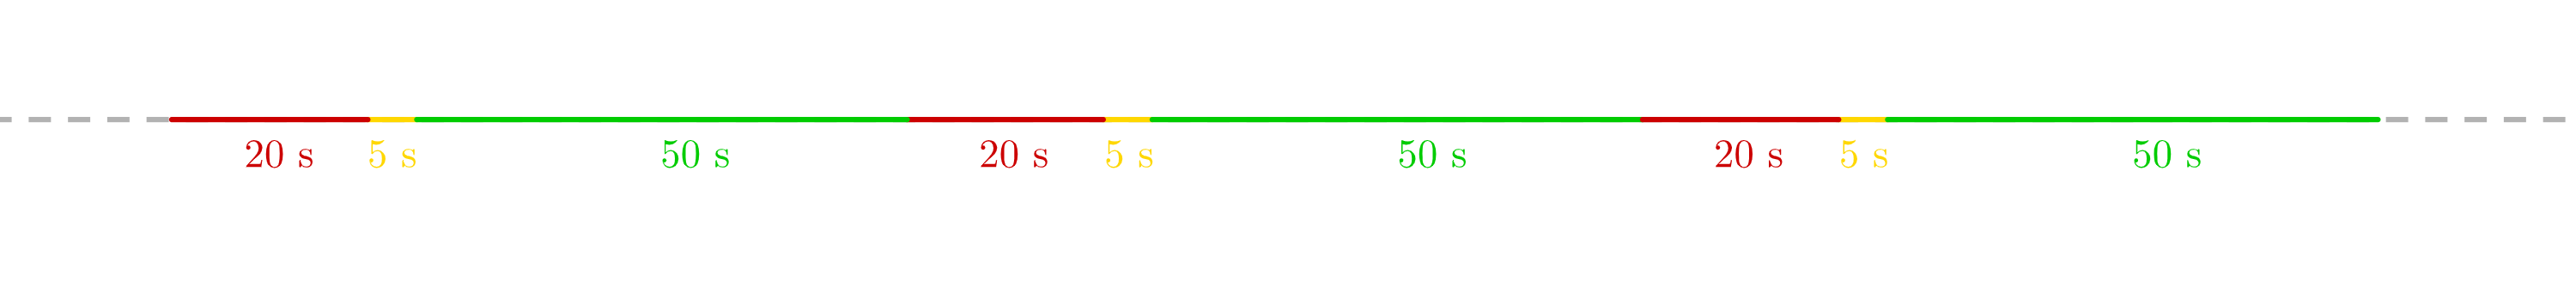
\includegraphics[width=1\linewidth]{figs/solution_light.png}}
% \\~\\
% Because there are $50$ seconds of green in every segment of time with $75$ seconds length, the probability of passing under green light would be $\dfrac{50}{75} = \dfrac{2}{3}$.

% \end{solution}

% \smallskip

% \begin{solution}

% Let $X$ denote the number of the first burned photo in the roll. Clearly, $X$ can have the values $1$ to $21$ each with an equal probability $\dfrac{1}{21}$.

% \begin{enumerate}
%     \item[a) ] For the eighth photo to be burn, $X$ should be one of $\{5, 6, 7, 8\}$; similarly for the ninth it should be one of $\{6, 7, 8, 9\}$; and for the tenth, one of $\{7, 8, 9, 10\}$. We get:
%     \[
%         \PP(X\in \{5, 6, 7, 8\} \cup \{6,7,8,9\}\cup\{7,8, 9, 10\}) = \PP(X\in \{5, 6, 7, 8, 9, 10\}) = \dfrac{6}{21} = \dfrac{2}{7}.
%     \]
    
%     \item[b) ] Similarly, for all three of them to be burned, we have:
%     \[
%         \PP(X\in \{5, 6, 7, 8\} \cap \{6,7,8,9\}\cap\{7,8, 9, 10\}) = \PP(X\in \{7, 8\}) = \dfrac{2}{21}.
%     \]
% \end{enumerate}

% \end{solution}


% \smallskip

% \begin{solution}
% We can represent the problem on a coordinate
% system, by letting $x$ denote the time Anush arrives, and $y$, the time Nairi arrives. Since either of them may arrive at any time within the entire hour, the sample space may be
% represented as the square $\Omega = [0,60]\times [0,60]$. The area of the sample space is, thus, $|\Omega|=60^2=3600$.

% The feasible region is found by representing the 15-minute waiting
% period. There are two cases:
% \begin{enumerate}
%     \item[a) ] If Nairi arrives first, then Anush ($x$) and Nairi ($y$) will meet if $y - x < 15$;
    
%     \item[b) ] If Anush arrives first, then Anush ($x$) and Nairi ($y$) will meet if $x - y < 15$.
% \end{enumerate}

% 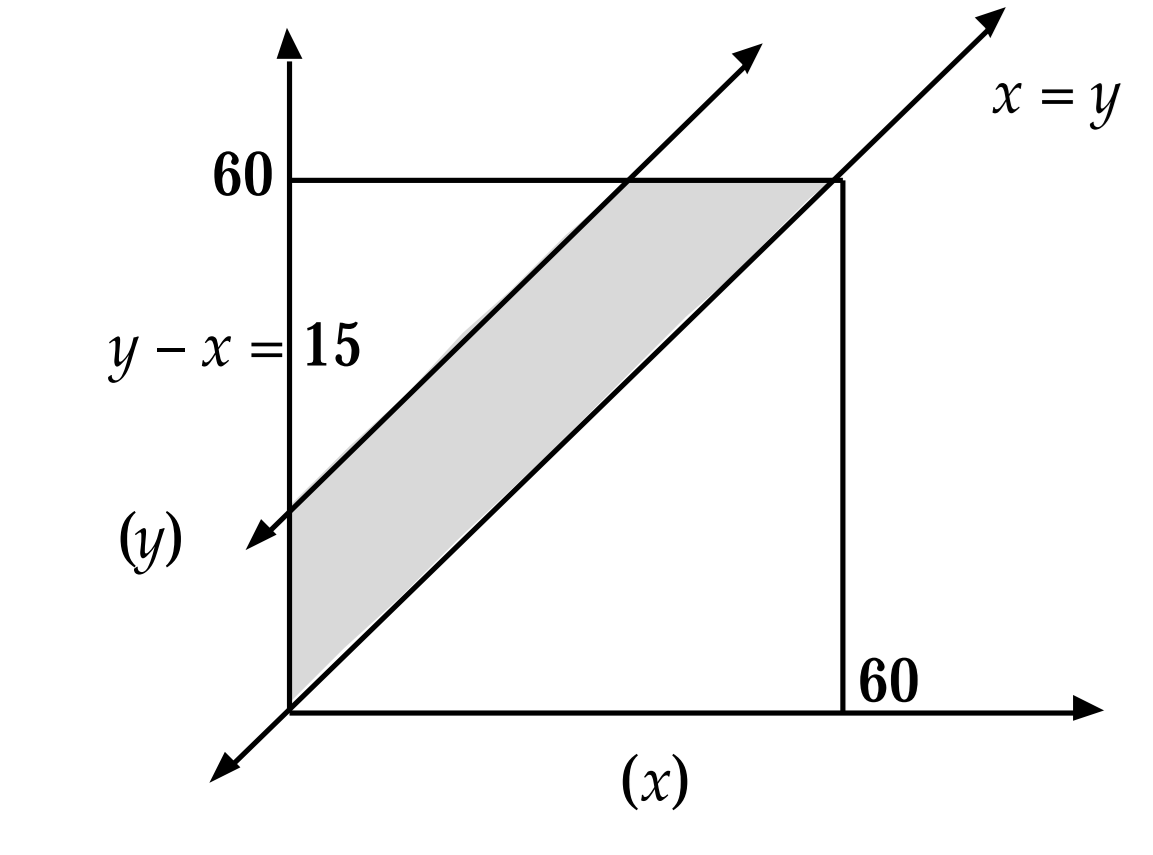
\includegraphics[width=0.4\linewidth]{figs/region2.png}
% 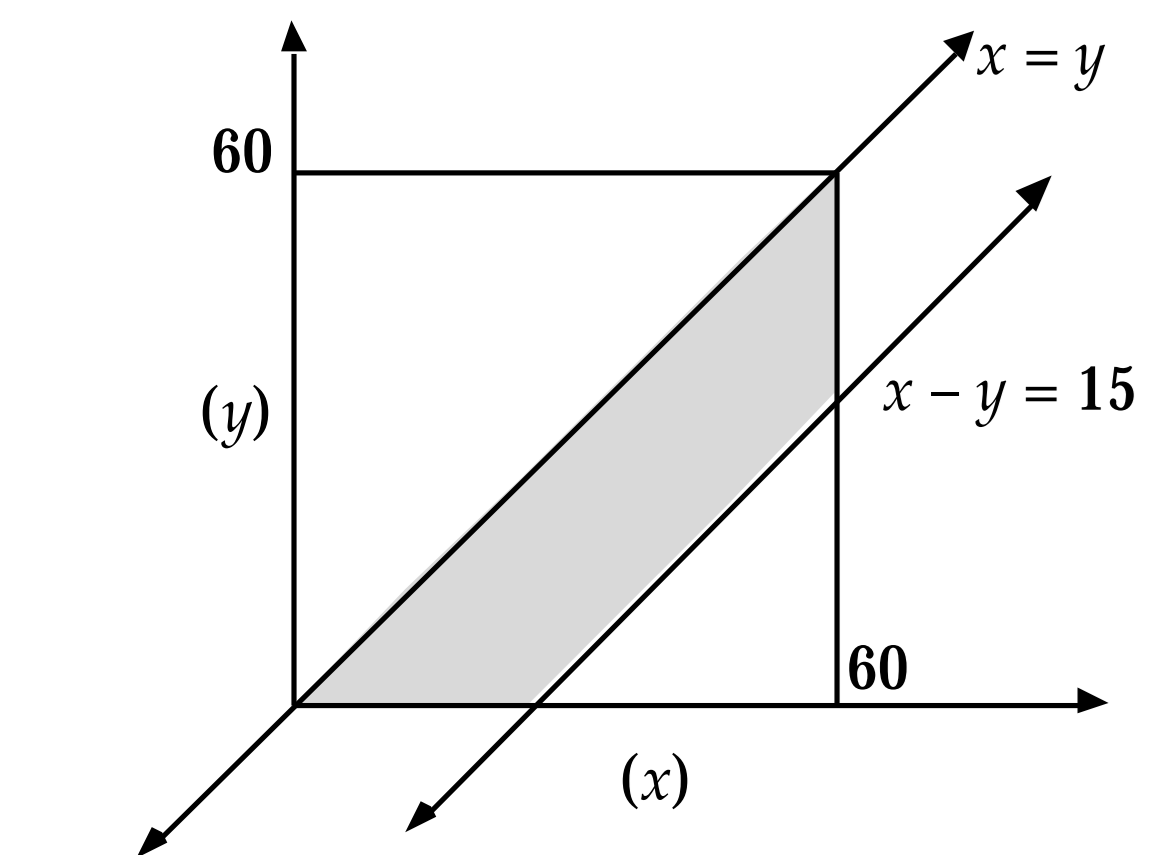
\includegraphics[width=0.4\linewidth]{figs/region1.png}
% \\
% \begin{center}
%     \textit{
% \qquad  a) Nairi arrives first \qquad  \qquad \qquad \quad b) Anush arrives first \qquad\qquad\qquad}
% \end{center}

% \newpage

% The union of the two shaded areas is the feasible region. If the
% arrival times of the two can be represented by a point within
% either shaded area, then they will meet. Calculating the shaded area and dividing it by the area of the sample space, we get:
% \[
% \PP(\text{Nairi and Anush will meet}) = \PP(|x-y|<15) = \dfrac{60^2-45^2}{60^2} = \dfrac{1575}{3600} = 0.4375.
% \]

% \begin{figure}
%     \centering
% 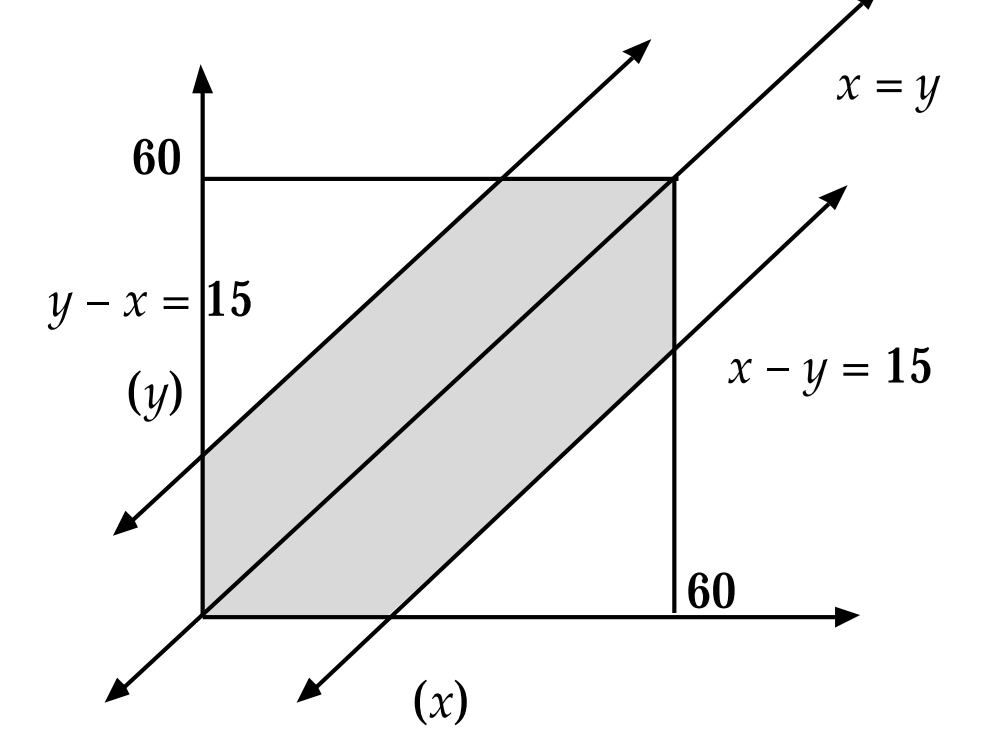
\includegraphics[width=0.4\linewidth]{figs/region3.png}
% \end{figure}

% \end{solution}


% \smallskip

% \begin{solution}

% When we put two points (let's say $B$ and $C$) on a segment (say, $AD=8$) we get three segments. Let's denote their lengths by $x$, $y$ and $8-x-y$:
%   \begin{center}
%    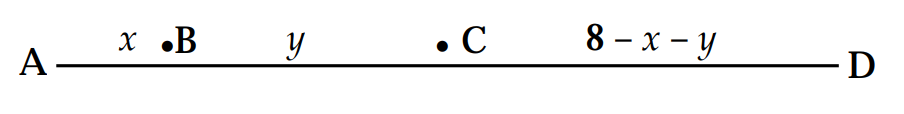
\includegraphics[width=0.5\linewidth]{figs/line1.png}
%   \end{center}

% The length of $AB$ must be less than 8 cm, and the
% length of $BC$ must be less than 8 cm too. In addition, their also must be less than the total
% length of the original segment, so $AB + BC$ is less than 8 cm. Thus, $x$ and $y$ should satisfy the following inequalities:
% \[
% \begin{cases}
%     x < 8 \\
%     y < 8 \\
%     x+y < 8
% \end{cases}
% \quad\Leftrightarrow \quad\begin{cases}
%     x < 8 \\
%     y < 8 \\
%     y < 8-x
% \end{cases}
% \]

% The shaded region ($QRS$) will be our sample space:
% \begin{center}
%     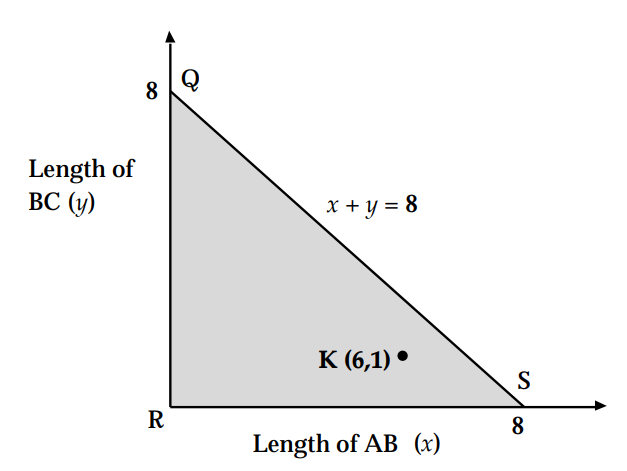
\includegraphics[width=0.4\linewidth]{figs/line2.png}
% \end{center}
% with the area $\dfrac{8\cdot 8 }{2}=32$. 

% Now, for a triangle with sides $x$, $y$, $8-x-y$ to exist, the following inequalities must hold:
% \[
% \begin{cases}
%     AB+BC>CD\\
%     AB+CD>BC\\
%     BC+CD>AB
% \end{cases}\quad\Leftrightarrow\quad
% \begin{cases}
%     x + y > 8 - x - y \\
%     x + (8 -x -y) > y\\
%     y + (8 - x - y) > x 
% \end{cases}
% \]
% which simplify to:
% \[
% \begin{cases}
%     y>4-x\\
%     y<4\\
%     x<4
% \end{cases}
% \]

% Drawing the region determined by these inequalities (i.e. the set of all $(x,y)$ points satisfying them), we get the following triangle $EFG$:
% \begin{center}
%     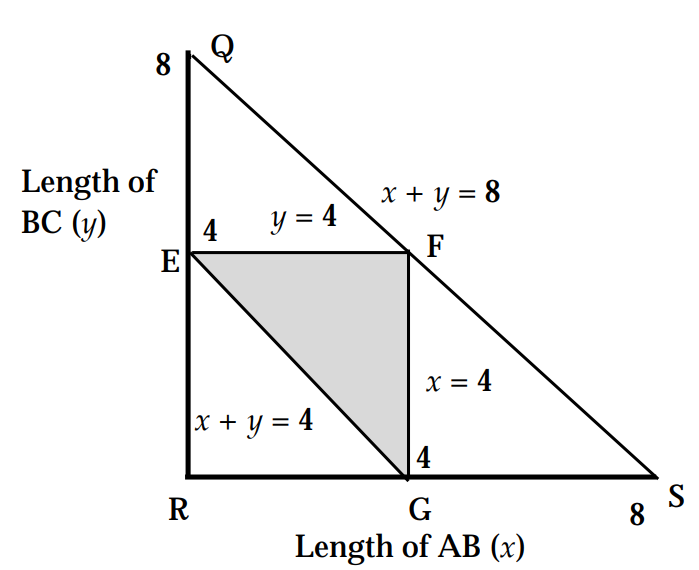
\includegraphics[width=0.36\linewidth]{figs/line3.png}
% \end{center}

% Therefore, the probability that 3 randomly selected segments will form a triangle is $\dfrac{8}{32}=0.25$.


% \end{solution}


% \smallskip

% \begin{solution}
% Let $X$ denote the number on the die. After Vahe doing the magic, the possible values $X$ can take are $2$ and $6$ each with probability $\dfrac{1}{6}$, and $3$ and $5$ each with probability $\dfrac{2}{6}$. In other words, the PMF of $X$ is:
% \[
% \PP(X=k) = \begin{cases}
%     1/6, & k\in\{2,6\} \\
%     2/6, & k\in\{3,5\} \\
%     0, & \text{otherwise}
% \end{cases}
% \]

% Therefore,
% \[
% \mathbb{E}(X) = 2 \cdot \dfrac{1}{6}  + 3 \cdot \dfrac{2}{6} + 5 \cdot \dfrac{2}{6} + 6 \cdot \dfrac{1}{6}   = 4.
% \]

% To calculate $\operatorname{Var}(X)=\mathbb{E}(X^2) - (\mathbb{E}(X))^2$, we should also calculate $\mathbb{E}(X^2)$:
% \begin{align*}
%     & \mathbb{E}(X^2) = 2^2 \cdot \dfrac{1}{6}  + 3^2 \cdot \dfrac{2}{6} + 5^2 \cdot \dfrac{2}{6} + 6^2 \cdot \dfrac{1}{6}   = 18, \\
%     & \operatorname{Var}(X) =\mathbb{E}(X^2) - (\mathbb{E}(X))^2= 18 - 4^2 = 2.
% \end{align*}

% \end{solution}

% \smallskip

% \begin{solution}
% \begin{enumerate}
%     \item[a) ] With the same steps as in the previous problem,
%     \begin{align*}
%     & \mathbb{E}(X) = \int_{-\infty}^\infty xf(x)\,dx
%                      = \int_{0}^1 x\cdot 2x \, dx
%                      = \dfrac{2}{3} x^3\bigg\vert_{0}^{1} = \dfrac{2}{3},
%     \\
%     & \mathbb{E}(X^2) = \int_{-\infty}^\infty x^2f(x)\,dx
%                      = \int_{0}^1 x^2\cdot 2x \, dx
%                      = \dfrac{2}{4} x^4\bigg\vert_{0}^{1} = \dfrac{1}{2},
%     \\
%     & \operatorname{Var}(X) =\mathbb{E}(X^2) - (\mathbb{E}(X))^2= \dfrac{1}{2}-\left(\dfrac{2}{3}\right)^2 = \dfrac{1}{18}.
%     \end{align*}
    
%     \item[b) ] Since we already have $\mathbb{E}(X)$ and since expectation is a linear function:
%     \[
%     \mathbb{E}(2X) = 2 \cdot \mathbb{E}(X) = \dfrac{4}{3},
%     \]
%     and since $\operatorname{Var}(aX)=a^2\cdot \operatorname{Var}(X)$ for all $a\in\R$,
%     \[
%     \operatorname{Var}(2X) = 4\cdot\operatorname{Var}(X) = \dfrac{2}{9}.
%     \]
        
%     \item[c) ] By the same logic, due to the linearity of expectation,
%     \[
%     \mathbb{E}(2X+7)=\mathbb{E}(2X)+7= 7\dfrac{4}{3}.
%     \]

%     As for $\operatorname{Var}(2X+7)$, after adding $7$ to $2X$, all of its values, as well as its expectation, increase by the same amount; therefore, its variance (the average squared distance between its values and their mean) should not change after adding $7$. Indeed,
%     \[
%     \operatorname{Var}(2X+7) = \mathbb{E}\big((2X+7 - \mathbb{E}(2X+7))^2\big) 
%      = \mathbb{E}\big((2X+7 - \mathbb{E}(2X) - 7)^2\big) 
%      = \mathbb{E}\big((2X- \mathbb{E}(2X) )^2\big),
%     \]
%     which equals $\operatorname{Var}(2X) = \dfrac{2}{9}$ by its definition.
    
% \end{enumerate}

% \end{solution}

    % \begin{center}\begin{large} Solutions 6, Probability theory continued
 \end{large}\end{center}
 \bigskip

\tableofcontents

% 1
\section{Pencils in the boxes}
\begin{problem} % 1
There are two boxes containing $\{5, 11, 8\}$ and $\{10, 8, 6\}$ white, black, red pencils respectively. One pencil is drawn from each box. What is the probability that the pencils have the same color?
\end{problem}
\bigskip

\begin{solution} % 1
Let's denote the event of drawing a white, black, red ball from the first box by $W_1$, $B_1$, $R_1$, respectively; and $W_2$, $B_2$, $R_2$ for the second box. Then the event of having two balls of the same color is equivalent to either having two whites, or two blacks, two reds. Therefore,
\begin{align*}
    \PP\big((W_1\cap W_2) &\text{ or } (B_1\cap B_2) \text{ or } (R_1\cap R_2) \big) \\&= \PP\big(W_1\cap W_2)+\PP(B_1\cap B_2) +\PP(R_1\cap R_2) \\&= \PP\big(W_1)\PP(W_2)+\PP(B_1)\PP(B_2) +\PP(R_1) \PP(R_2) \\&= \dfrac{5}{24}\cdot \dfrac{10}{24} +  \dfrac{11}{24}\cdot \dfrac{8}{24} +  \dfrac{8}{24}\cdot \dfrac{6}{24} = \dfrac{186}{576} = \dfrac{31}{96} 
\end{align*}

An alternative approach would be counting all $24\times 24$ pairs and calculating the probability of one-colored pairs.
\end{solution}

% 2
\section{Questions on exam}
\begin{problem} % 2
Suppose that you know the answers to 20 questions out of the total 25
questions in the entrance examination, from which you are only asked
3 random questions. What is the probability that you answer all of
the questions?
\end{problem}
\bigskip
\begin{solution}
For us to answer all 3 questions correctly, they have to be from the 20 questions we have learned. Let $Q_1, Q_2, Q_3$ be the events of the first, second, third questions being from the questions we know. Then
\[\PP(Q_1 \cap Q_2 \cap Q_3) = \PP(Q_1)\cdot \PP(Q_2\mid Q_1)\cdot \PP(Q_3 \mid Q_1, Q_2) = \dfrac{20}{25}\dfrac{19}{24}\dfrac{18}{23} = \dfrac{57}{115}. \]

Or we can just calculate the number of all possible triplets: $C_{25}^{3}$, the number of triplets from questions we know: $C_{20}^{3}$, and divide the latter one by the former:
\[
\dfrac{C_{20}^{3}}{C_{25}^{3}} = \dfrac{57}{115}.
\]
\end{solution}

% 3
\section{Balls in a box}
\begin{problem} % 3
There are two boxes containing {5, 11} and {10, 8} white, black balls
respectively. First, we take out a ball from each of the boxes. Then, we randomly choose one of them. What is the probability that the
final ball is white?
\end{problem}
\bigskip
\begin{solution}
Let $X$ be 1 if the ball from the first box is white, otherwise 0; and define $Y$ for the second box analogously. Denote by $W$ the event (not an RV!) of choosing a white ball on the final step.

\begin{align*}
    \PP(W) &= \PP(W\mid X=1, Y=1)\cdot \PP(X=1,Y=1) \\&+
\PP(W\mid X=0, Y=1)\cdot \PP(X=0,Y=1)\\&+
\PP(W\mid X=1, Y=0)\cdot \PP(X=1,Y=0)\\&+
\PP(W\mid X=0, Y=0)\cdot \PP(X=0,Y=0)
\end{align*}

The last case is impossible because we can't choose a white ball from two black balls. Therefore:
\begin{align*}
     \PP(W) &= \PP(W\mid X=1, Y=1)\cdot \PP(X=1,Y=1) \\&+
\PP(W\mid X=0, Y=1)\cdot \PP(X=0,Y=1)\\&+
\PP(W\mid X=1, Y=0)\cdot \PP(X=1,Y=0)\\&=
1\cdot \PP(X=1)\PP(Y=1) +\dfrac{1}{2}\cdot \PP(X=0)\PP(Y=1)+
\dfrac{1}{2}\cdot \PP(X=1)\PP(Y=0)\\&=
\dfrac{5}{15}\dfrac{11}{19}+\dfrac{1}{2}\dfrac{10}{15}\dfrac{11}{19}+
\dfrac{1}{2}\dfrac{5}{15}\dfrac{8}{19}=\dfrac{26}{57}
\end{align*}
\end{solution}

% 4
\section{Balls in a box (performing steps in order)}
\begin{problem} % 4
There are three boxes having 4 white and 6 black balls in each of them.
Suppose we perform the following steps in the given order:
    \begin{enumerate}
        \item[a) ] take out a ball from the first box and put it into the second one,
        \item[b) ] take out a ball from the second box and put it into the third one,
        \item[c) ] take out a ball from the third box and put it into the first one.
    \end{enumerate}
    What is the probability of taking a white ball from the third box (after doing \textit{a)-c)})?
\end{problem}
\bigskip

\begin{solution} % 4
Let $W_1$ denote the event that we have taken out a white ball from the first box and put into the second one; similarly define $B_1, \dots, W_3$. Also denote by $\tilde{W}$ the event that after steps 1-3, we take a white ball from the third ball.

We have:
\begin{align*}
    &\PP(W_1) = \dfrac{4}{10}= \dfrac{2}{5},\\
    &\PP(B_1) = \dfrac{6}{10}= \dfrac{3}{5},\\
    &\PP(W_2) = \PP(W_2\mid W_1)\PP(W_1)+\PP(W_2\mid B_1)\PP(B_1)=\dfrac{5}{11}\dfrac{4}{10}+\dfrac{4}{11}\dfrac{6}{10}=\dfrac{2}{5},\\
    &\PP(B_2) =1-\PP(W_2)=\dfrac{3}{5}.\\
    % &\PP(W_3) = \PP(W_3\mid W_2)\PP(W_2)+\PP(W_3\mid B_2)\PP(B_2)=\dfrac{2}{5},\\
    % &\PP(B_3) =1-\PP(W_3)=\dfrac{3}{5}.\\
\end{align*}

The probability of taking out a white ball from the third box depends on the color of the balls put into it (step 2) and taken out from it (step 3). Thus, 
\begin{align*}
     \PP(\tilde{W}) &= \PP(\tilde{W}\mid W_2, W_3)\cdot \PP( W_2, W_3) \\&+
     \PP(\tilde{W}\mid W_2, B_3)\cdot \PP( W_2, B_3) \\&+
     \PP(\tilde{W}\mid B_2, W_3)\cdot \PP( B_2, W_3) \\&+
     \PP(\tilde{W}\mid B_2, B_3)\cdot \PP( B_2, B_3) \\&=
     \PP(\tilde{W}\mid W_2, W_3)\cdot \PP(W_3\mid W_2) \cdot \PP( W_2) \\&+
     \PP(\tilde{W}\mid W_2, B_3)\cdot \PP(B_3\mid W_2) \cdot \PP( W_2)\\&+
     \PP(\tilde{W}\mid B_2, W_3)\cdot \PP(W_3\mid B_2) \cdot \PP( B_2) \\&+
     \PP(\tilde{W}\mid B_2, B_3)\cdot \PP(B_3\mid B_2) \cdot \PP( B_2) \\&=     
\dfrac{4}{10}\dfrac{5}{11}\dfrac{2}{5} +
\dfrac{5}{10}\dfrac{6}{11}\dfrac{2}{5} +
\dfrac{3}{10}\dfrac{4}{11}\dfrac{3}{5} +
\dfrac{4}{10}\dfrac{7}{11}\dfrac{3}{5} =\dfrac{220}{550} = \dfrac{2}{5}.
\end{align*}
\end{solution}

% 5
\section{Weapon producing factory}
\begin{problem} % 5
Two factories produce similar weapons and deliver it to the army warehouse. The first factory’s productivity is two times more than that of
the second one. Moreover, $40\%$ of the weapons produced by the first
factory have some defects, while the same indicator is only $16\%$ for
the second factory. We randomly take a weapon from the warehouse,
test it and it appears to have no defects. What is the probability that
the weapon was produced by the first factory?
\end{problem}
\bigskip

\begin{solution} % 5
Let $F_1$ denote the event that a randomly taken weapon is produced in the first factory, $F_2$ in the second; and let $D$ be the event of it having a defect.

We have:
\begin{align*}
    &\PP(F_1) = \dfrac{2}{3},&\qquad &\PP(F_2) = \dfrac{1}{3}&\\
    &\PP(D\mid F_1) = 0.4= \dfrac{2}{5},&\qquad &\PP(D\mid F_2) = 0.16= \dfrac{4}{25},
\end{align*}
hence 
\[\PP(D) = \PP(D\mid F_1)\PP(F_1)+\PP(D\mid F_2)\PP(F_2)=\dfrac{8}{25}.\]

Using Bayes' rule, we get:
\begin{align*}
     \PP(F_1 \mid D^C) = \dfrac{\PP(F_1)}{\PP(D^C)}
     \PP(D^C \mid F_1)=\dfrac{2/3}{17/25}\cdot \dfrac{3}{5}=\dfrac{10}{17}.
\end{align*}
\end{solution}


% 6
\section{Color-blind person's gender}
\begin{problem} % 6
According to some statistics, $5\%$ of all males and $0.25\%$ of all females
are color-blind. Assuming that the populations of males and females
are equal, what is the probability that a randomly chosen color-blind person is a male?
\end{problem}
\bigskip
\begin{solution} % 6
Let $F$ denote the event that a randomly taken person is female, $M$ male; and let $C$ be the event they are color-blind.

We have:
\begin{align*}
    &\PP(F)=\PP(M) = 0.5,\\
    &\PP(C\mid F) = 0.0025,\\
    &\PP(C\mid M) = 0.05,
\end{align*}
hence 
\[\PP(C) = \PP(C\mid F)\PP(F)+\PP(C\mid M)\PP(M)=0.02625.\]

Using Bayes' rule, we get:
\begin{align*}
     \PP(M \mid C) = \dfrac{\PP(M)}{\PP(C)}
     \PP(C \mid M)=\dfrac{0.5}{0.02625}\cdot0.05\approx 0.95.
\end{align*}
\end{solution}
  

% 7
\section{Late for work}
\begin{problem} % 7
    Nune uses her car $30\%$ of the time, walks $30\%$ of the time and rides the bus $40\%$ of the time as she goes to work. She is late $10\%$ of the time when she walks, $3\%$ of the time when she drives, and $7\%$ of the time she takes the bus.
    \begin{enumerate}
        \item[a) ] What is the probability she took the bus if she was late?
        
        \item[b) ] What is the probability she walked if she is on time?
    \end{enumerate}
\end{problem}
\bigskip
\begin{solution} % 7
    Let $C, W$ and $B$ denote the events of Nune going by car, walking or bus respectively; and let $L$ denote the event of her being late. Then,
    \[
    \displaystyle{\PP(B\mid L) = \frac{\PP(L\mid B) \PP(B)}{\PP(L)}= \frac{0.4 \cdot 0.07}{0.4 \cdot 0.07 +0.3 \cdot 0.03+0.3\cdot 0.1} \approx 0.418.}
    \]
\end{solution}

% 8
\section{Traffic light}
\begin{problem} % 8
    On the way to the ACA, your
bus passes through a traffic light. The light cycle of the traffic light is $20$
seconds red, $5$ seconds yellow, and $50$ seconds green. What is the
probability that you will pass under a green light?
\end{problem}
\bigskip
\begin{solution} % 8
Let's draw time as an infinite line and mark the $20$, $5$ and $50$ second segments between which the traffic light is constantly switching:
\\~\\
{    \centering
    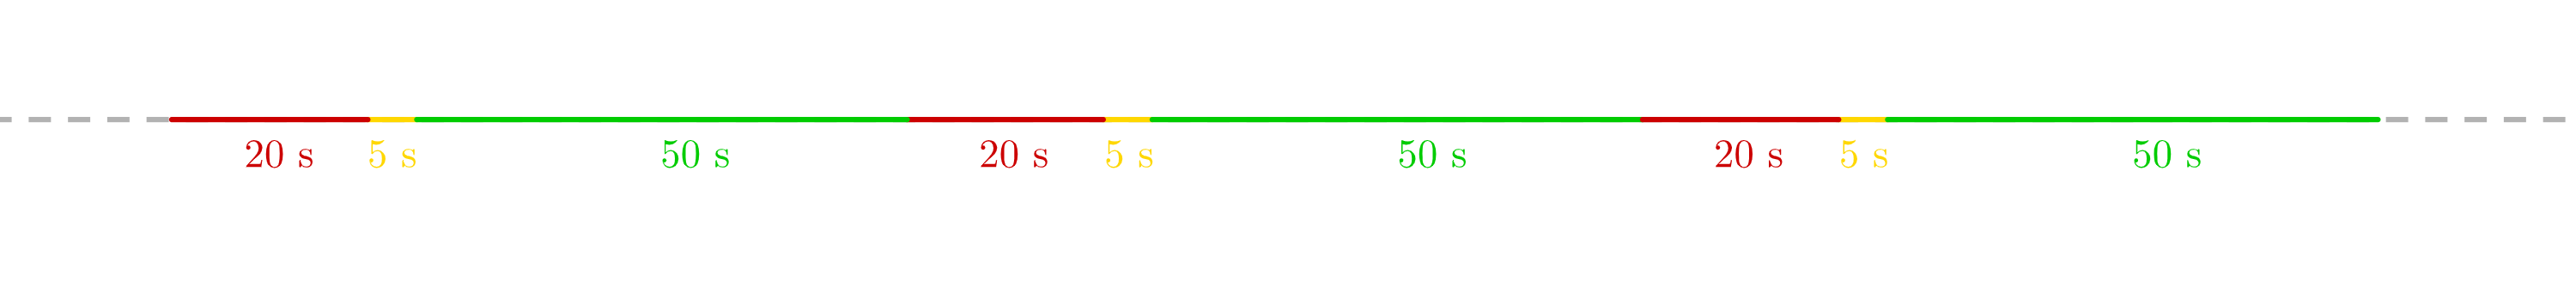
\includegraphics[width=1\linewidth]{figs/solution_light.png}}
\\~\\
Because there are $50$ seconds of green in every segment of time with $75$ seconds length, the probability of passing under green light would be $\dfrac{50}{75} = \dfrac{2}{3}$.

\end{solution}

% 9
\section{Camera film}
\begin{problem} % 9
After a trip to Garni-Geghard, you bring your camera film to a photography shop. Unfortunately, the shop ruins $4$ photos in a row from your roll which contains $24$ photos. What is the probability that the ruined photos included the
\begin{enumerate}
    \item[a) ] eighth, ninth or tenth photos,
    \item[b) ] eighth, ninth and tenth photos
\end{enumerate}
on the roll (the photos of the Garni Temple)?
\end{problem}
\bigskip
\begin{solution} % 9
Let $X$ denote the number of the first burned photo in the roll. Clearly, $X$ can have the values $1$ to $21$ each with an equal probability $\dfrac{1}{21}$.
\begin{enumerate}
    \item[a) ] For the eighth photo to be burn, $X$ should be one of $\{5, 6, 7, 8\}$; similarly for the ninth it should be one of $\{6, 7, 8, 9\}$; and for the tenth, one of $\{7, 8, 9, 10\}$. We get:
    \[
        \PP(X\in \{5, 6, 7, 8\} \cup \{6,7,8,9\}\cup\{7,8, 9, 10\}) = \PP(X\in \{5, 6, 7, 8, 9, 10\}) = \dfrac{6}{21} = \dfrac{2}{7}.
    \]
    
    \item[b) ] Similarly, for all three of them to be burned, we have:
    \[
        \PP(X\in \{5, 6, 7, 8\} \cap \{6,7,8,9\}\cap\{7,8, 9, 10\}) = \PP(X\in \{7, 8\}) = \dfrac{2}{21}.
    \]
\end{enumerate}

\end{solution}


% 10
\section{Meeting at shopping center}
\begin{problem} % 10
Anush and Nairi are shopping at the mall. They agree to split up for a time and then meet for lunch. They plan to meet in
front of Kinopark between 12:00 and 13:00. The one who arrives first agrees to wait $15$ minutes for the other to arrive. After $15$
minutes, that person will leave and continue shopping. What is the probability that they will meet if each one of them arrives at any time between 12:00 and 13:00?

\textit{Hint: Try to represent the problem on coordinate system, by letting
$x$ denote the time Anush arrives, and $y$, the time Nairi arrives.}
\end{problem}
\bigskip
\begin{solution} % 10
We can represent the problem on a coordinate
system, by letting $x$ denote the time Anush arrives, and $y$, the time Nairi arrives. Since either of them may arrive at any time within the entire hour, the sample space may be
represented as the square $\Omega = [0,60]\times [0,60]$. The area of the sample space is, thus, $|\Omega|=60^2=3600$.

The feasible region is found by representing the 15-minute waiting
period. There are two cases:
\begin{enumerate}
    \item[a) ] If Nairi arrives first, then Anush ($x$) and Nairi ($y$) will meet if $y - x < 15$;
    
    \item[b) ] If Anush arrives first, then Anush ($x$) and Nairi ($y$) will meet if $x - y < 15$.
\end{enumerate}

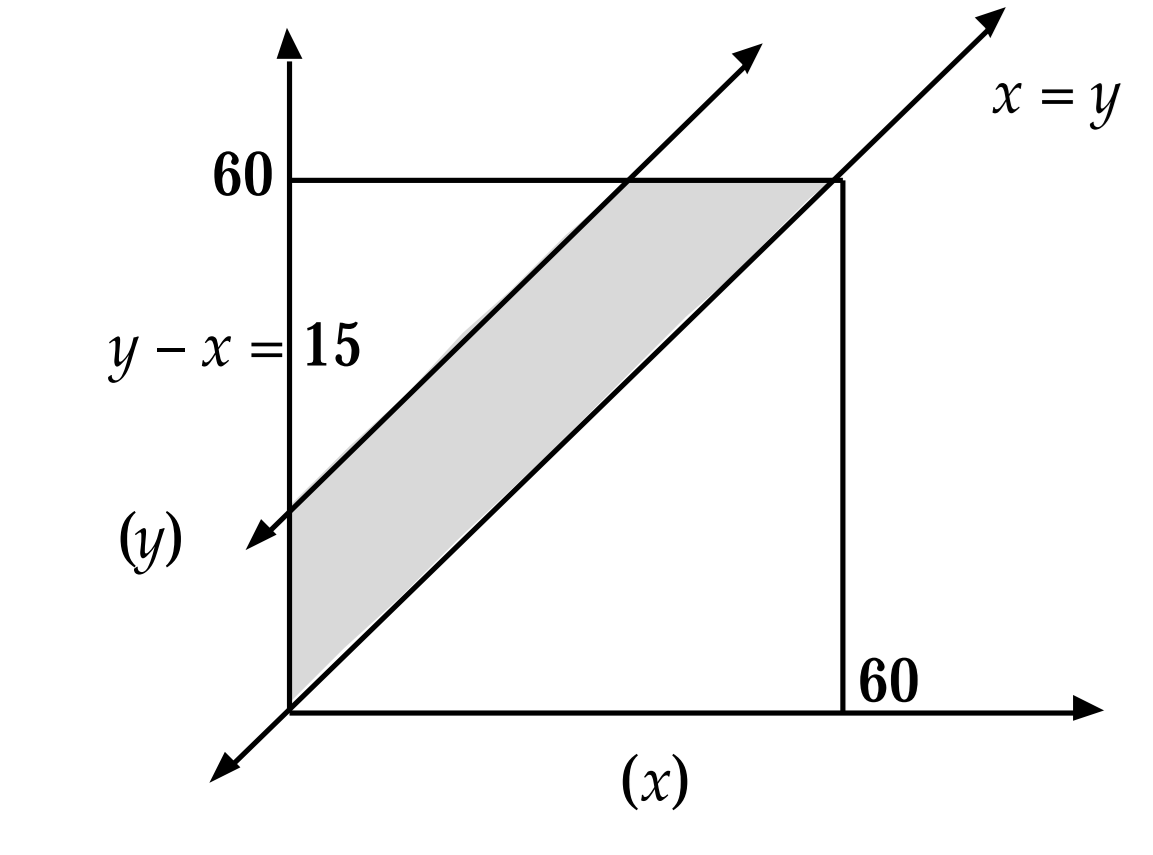
\includegraphics[width=0.4\linewidth]{figs/region2.png}
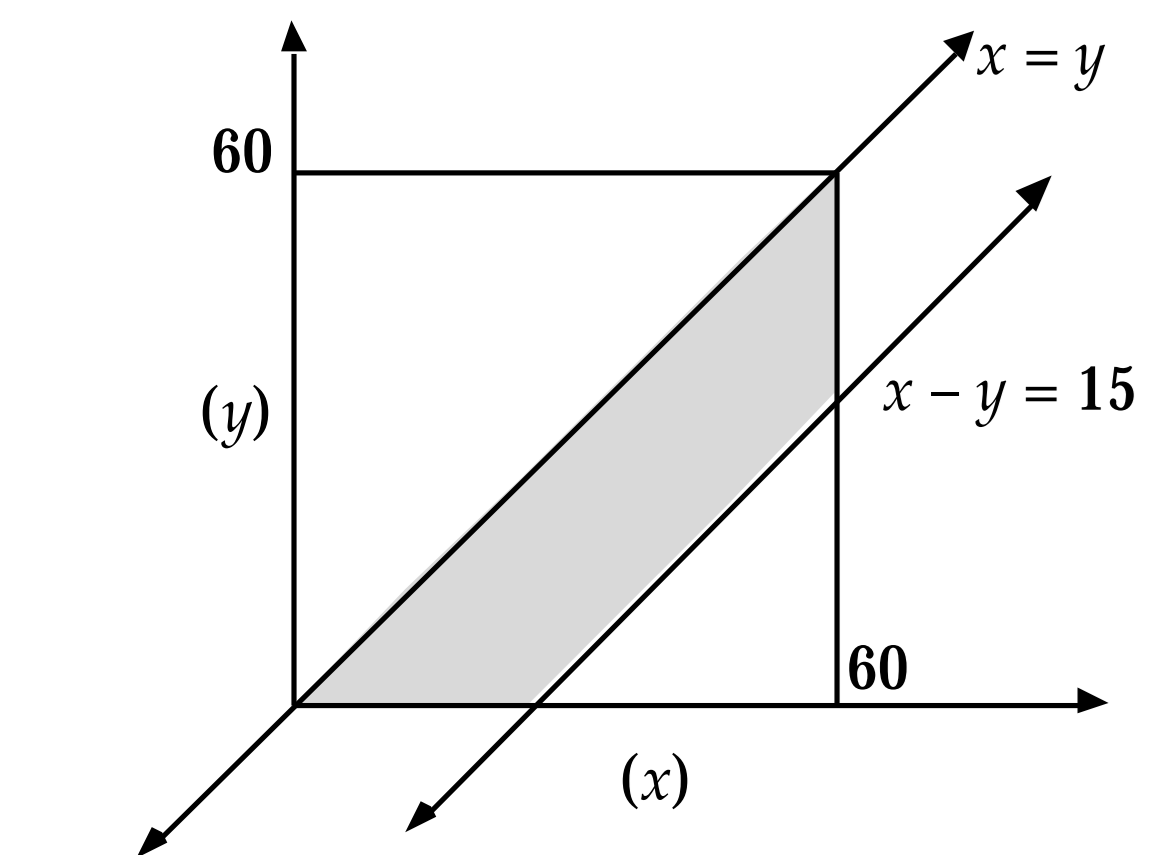
\includegraphics[width=0.4\linewidth]{figs/region1.png}
\\
\begin{center}
    \textit{
\qquad  a) Nairi arrives first \qquad  \qquad \qquad \quad b) Anush arrives first \qquad\qquad\qquad}
\end{center}

The union of the two shaded areas is the feasible region. If the
arrival times of the two can be represented by a point within
either shaded area, then they will meet. Calculating the shaded area and dividing it by the area of the sample space, we get:
\[
\PP(\text{Nairi and Anush will meet}) = \PP(|x-y|<15) = \dfrac{60^2-45^2}{60^2} = \dfrac{1575}{3600} = 0.4375.
\]

\begin{figure}
    \centering
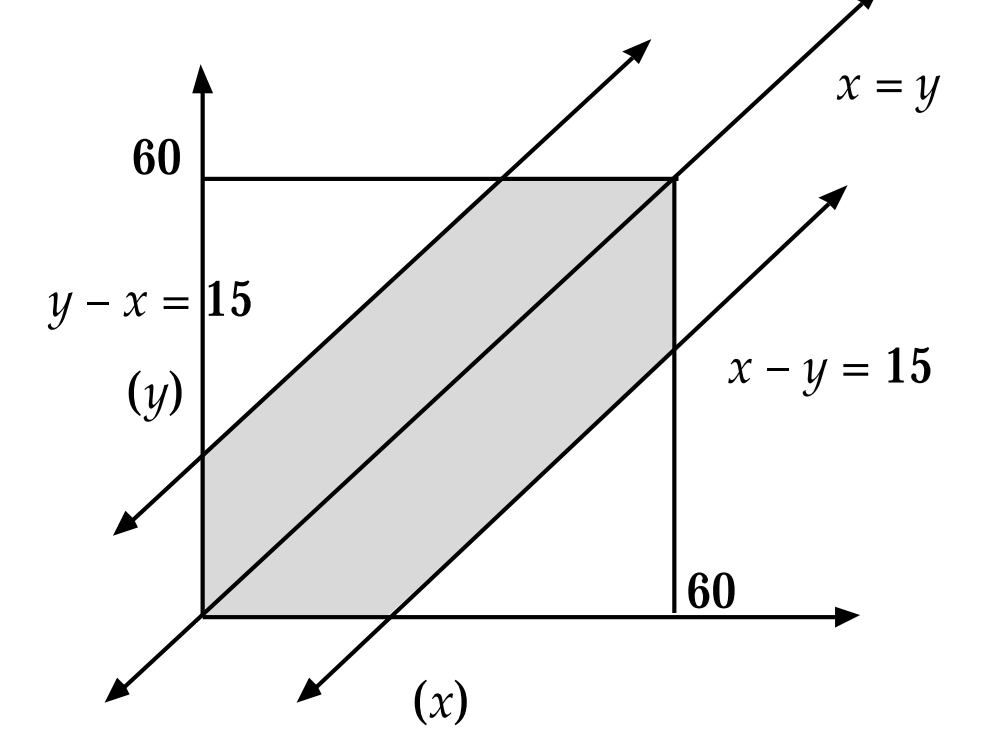
\includegraphics[width=0.4\linewidth]{figs/region3.png}
\end{figure}

\end{solution}

% 11
\section{Triangle formed by line segments}
\begin{problem} % 11
    A line segment is $8$ cm long. Two points are put on the segment at
random locations. What is the probability that the three segments formed by
the two points can make a triangle?
\end{problem}
\bigskip
\begin{solution} % 11
When we put two points (let's say $B$ and $C$) on a segment (say, $AD=8$) we get three segments. Let's denote their lengths by $x$, $y$ and $8-x-y$:
  \begin{center}
   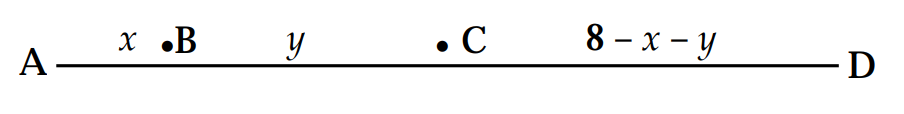
\includegraphics[width=0.5\linewidth]{figs/line1.png}
  \end{center}

The length of $AB$ must be less than 8 cm, and the
length of $BC$ must be less than 8 cm too. In addition, their also must be less than the total
length of the original segment, so $AB + BC$ is less than 8 cm. Thus, $x$ and $y$ should satisfy the following inequalities:
\[
\begin{cases}
    x < 8 \\
    y < 8 \\
    x+y < 8
\end{cases}
\quad\Leftrightarrow \quad\begin{cases}
    x < 8 \\
    y < 8 \\
    y < 8-x
\end{cases}
\]

The shaded region ($QRS$) will be our sample space:
\begin{center}
    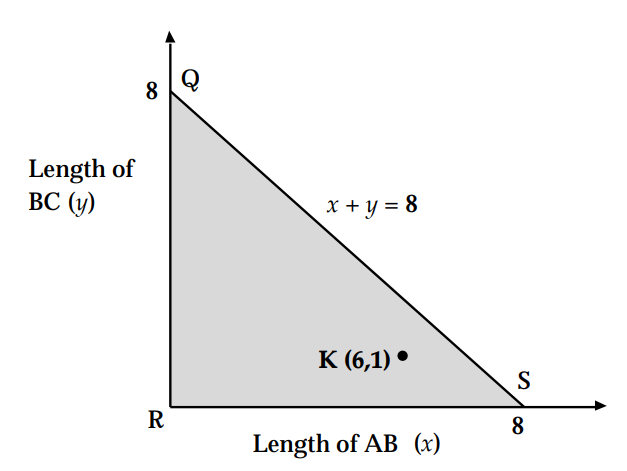
\includegraphics[width=0.4\linewidth]{figs/line2.png}
\end{center}
with the area $\dfrac{8\cdot 8 }{2}=32$. 

Now, for a triangle with sides $x$, $y$, $8-x-y$ to exist, the following inequalities must hold:
\[
\begin{cases}
    AB+BC>CD\\
    AB+CD>BC\\
    BC+CD>AB
\end{cases}\quad\Leftrightarrow\quad
\begin{cases}
    x + y > 8 - x - y \\
    x + (8 -x -y) > y\\
    y + (8 - x - y) > x 
\end{cases}
\]
which simplify to:
\[
\begin{cases}
    y>4-x\\
    y<4\\
    x<4
\end{cases}
\]

Drawing the region determined by these inequalities (i.e. the set of all $(x,y)$ points satisfying them), we get the following triangle $EFG$:
\begin{center}
    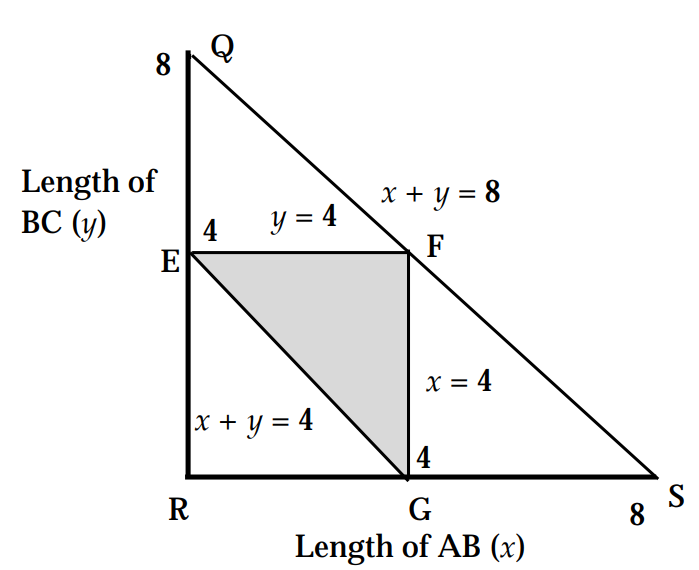
\includegraphics[width=0.36\linewidth]{figs/line3.png}
\end{center}

Therefore, the probability that 3 randomly selected segments will form a triangle is $\dfrac{8}{32}=0.25$.


\end{solution}

% 12
\section{Unusual rolling die}
\begin{problem} % 12
 Vahe added a dot on the   
\includegraphics[height=0.9em]{figs/4.png} side of the die, making it 
\includegraphics[height=0.9em]{figs/5.png}, and then added two dots on the 
\includegraphics[height=0.9em]{figs/1.png} side, making it 
\includegraphics[height=0.9em]{figs/3.png}.
   What is the probability that the outcome of the die is greater than $4$? Find the expectation and variance of the die.
\end{problem}
\bigskip
\begin{solution}
Let $X$ denote the number on the die. After Vahe doing the magic, the possible values $X$ can take are $2$ and $6$ each with probability $\dfrac{1}{6}$, and $3$ and $5$ each with probability $\dfrac{2}{6}$. In other words, the PMF of $X$ is:
\[
\PP(X=k) = \begin{cases}
    1/6, & k\in\{2,6\} \\
    2/6, & k\in\{3,5\} \\
    0, & \text{otherwise}
\end{cases}
\]

Therefore,
\[
\mathbb{E}(X) = 2 \cdot \dfrac{1}{6}  + 3 \cdot \dfrac{2}{6} + 5 \cdot \dfrac{2}{6} + 6 \cdot \dfrac{1}{6}   = 4.
\]

To calculate $\operatorname{Var}(X)=\mathbb{E}(X^2) - (\mathbb{E}(X))^2$, we should also calculate $\mathbb{E}(X^2)$:
\begin{align*}
    & \mathbb{E}(X^2) = 2^2 \cdot \dfrac{1}{6}  + 3^2 \cdot \dfrac{2}{6} + 5^2 \cdot \dfrac{2}{6} + 6^2 \cdot \dfrac{1}{6}   = 18, \\
    & \operatorname{Var}(X) =\mathbb{E}(X^2) - (\mathbb{E}(X))^2= 18 - 4^2 = 2.
\end{align*}

\end{solution}

% 13
\section{PDF of an RV}
\begin{problem} % 13
   Let $X$ be a random variable with the PDF:
   \[
   f(x) = \begin{cases}
       2x, & 0 \le x \le 1 \\
       0, & \text{otherwise}
   \end{cases}
   \]

   Find the expectation and variance of
   \begin{enumerate}
       \item[a) ] $X$,
       \item[b) ] $2X$,
       \item[c) ] $2X + 7$. 
       
   \end{enumerate}
\end{problem}
\bigskip
\begin{solution} % 13
\begin{enumerate}
    \item[a) ] With the same steps as in the previous problem,
    \begin{align*}
    & \mathbb{E}(X) = \int_{-\infty}^\infty xf(x)\,dx
                     = \int_{0}^1 x\cdot 2x \, dx
                     = \dfrac{2}{3} x^3\bigg\vert_{0}^{1} = \dfrac{2}{3},
    \\
    & \mathbb{E}(X^2) = \int_{-\infty}^\infty x^2f(x)\,dx
                     = \int_{0}^1 x^2\cdot 2x \, dx
                     = \dfrac{2}{4} x^4\bigg\vert_{0}^{1} = \dfrac{1}{2},
    \\
    & \operatorname{Var}(X) =\mathbb{E}(X^2) - (\mathbb{E}(X))^2= \dfrac{1}{2}-\left(\dfrac{2}{3}\right)^2 = \dfrac{1}{18}.
    \end{align*}
    
    \item[b) ] Since we already have $\mathbb{E}(X)$ and since expectation is a linear function:
    \[
    \mathbb{E}(2X) = 2 \cdot \mathbb{E}(X) = \dfrac{4}{3},
    \]
    and since $\operatorname{Var}(aX)=a^2\cdot \operatorname{Var}(X)$ for all $a\in\R$,
    \[
    \operatorname{Var}(2X) = 4\cdot\operatorname{Var}(X) = \dfrac{2}{9}.
    \]
        
    \item[c) ] By the same logic, due to the linearity of expectation,
    \[
    \mathbb{E}(2X+7)=\mathbb{E}(2X)+7= 7\dfrac{4}{3}.
    \]

    As for $\operatorname{Var}(2X+7)$, after adding $7$ to $2X$, all of its values, as well as its expectation, increase by the same amount; therefore, its variance (the average squared distance between its values and their mean) should not change after adding $7$. Indeed,
    \[
    \operatorname{Var}(2X+7) = \mathbb{E}\big((2X+7 - \mathbb{E}(2X+7))^2\big) 
     = \mathbb{E}\big((2X+7 - \mathbb{E}(2X) - 7)^2\big) 
     = \mathbb{E}\big((2X- \mathbb{E}(2X) )^2\big),
    \]
    which equals $\operatorname{Var}(2X) = \dfrac{2}{9}$ by its definition.
    
\end{enumerate}
\end{solution}



% \begin{solution}
%     Given that a dart always lands somewhere within the circular area with uniform probability, $|\Omega| = \pi \cdot 5^2 = 25\pi$. Then,

%     \begin{enumerate}
%         \item[a) ] $\PP(\text{circle 1}) = \dfrac{\pi \cdot 1^2}{|\Omega|} = \dfrac{1}{25}$,
        
%         \item[b) ] The total area of two red rings is $(\pi \cdot 4^2 - \pi \cdot 3^2) + (\pi \cdot 2^2 - \pi \cdot 1^2) = 10\pi$, hence  
%         $\PP(\text{red circle}) = \dfrac{10\pi}{|\Omega|} = \dfrac{10}{25} = \dfrac{2}{5}$,
        
%         \item[c) ] $\PP(\text{yellow circle}) = 1 - \PP(\text{red circle}) = \dfrac{3}{5}$.
%     \end{enumerate}
% \end{solution}


% \begin{solution}
% Let's denote the number of unique (distinct) colors of the 3 balls drawn by $X$. ($X$ is a random variable.)

% Then
% \[\PP(X\ge 2) = 1 - \PP(X<2) = 1-\PP(X=1),\]
% so its easier to calculate $\PP(X=1)$ (i.e. the probability that all 3 are of the same color), and subtract it from $1$. The same way as we calculated above, we can see that:
% \begin{align*}
%     \PP(X=1) &= \PP\big((W_1\cap W_2 \cap W_3) \text{ or } (B_1\cap B_2 \cap B_3) \text{ or } (R_1\cap R_2 \cap R_3) \big) \\&= \PP\big(W_1\cap W_2\cap W_3)+\PP(B_1\cap B_2\cap B_3) +\PP(R_1\cap R_2\cap R_3) \\&= 0+\dfrac{3}{10}\cdot \dfrac{2}{9} \cdot \dfrac{1}{8} +\dfrac{5}{10}\cdot \dfrac{4}{9} \cdot \dfrac{3}{8}  = \dfrac{66}{720} = \dfrac{11}{120} 
% \end{align*}
% \[
% \PP(X\ge 2) = 1-\dfrac{11}{120}  = \dfrac{109}{120}
% \]
% \end{solution}
% \smallskip



    %  \begin{center}\begin{large} Homework 6, Probability theory continued
 \end{large}\end{center}
 \bigskip

\bigskip

\tableofcontents

% 1
\section{Pencils in the boxes}
There are two boxes containing $\{5, 11, 8\}$ and $\{10, 8, 6\}$ white, black, red pencils respectively. One pencil is drawn from each box. What is the probability that the pencils have the same color?

% 2
\section{Questions on exam}
Suppose that you know the answers to 20 questions out of the total 25
questions in the entrance examination, from which you are only asked
3 random questions. What is the probability that you answer all of
the questions?

% 3
\section{Balls in a box}
There are two boxes containing {5, 11} and {10, 8} white, black balls
respectively. First, we take out a ball from each of the boxes. Then, we randomly choose one of them. What is the probability that the
final ball is white?

% 4
\section{Balls in a box (performing steps in order)}
There are three boxes having 4 white and 6 black balls in each of them.
Suppose we perform the following steps in the given order:
    \begin{enumerate}
        \item[a) ] take out a ball from the first box and put it into the second one,
        \item[b) ] take out a ball from the second box and put it into the third one,
        \item[c) ] take out a ball from the third box and put it into the first one.
    \end{enumerate}
    What is the probability of taking a white ball from the third box (after doing \textit{a)-c)})?


% 5
\section{Weapon producing factory}
Two factories produce similar weapons and deliver it to the army warehouse. The first factory’s productivity is two times more than that of
the second one. Moreover, $40\%$ of the weapons produced by the first
factory have some defects, while the same indicator is only $16\%$ for
the second factory. We randomly take a weapon from the warehouse,
test it and it appears to have no defects. What is the probability that
the weapon was produced by the first factory?

% 6
\section{Color-blind person's gender}
According to some statistics, $5\%$ of all males and $0.25\%$ of all females
are color-blind. Assuming that the populations of males and females
are equal, what is the probability that a randomly chosen color-blind person is a male?

% 7
\section{Late for work}
Nune uses her car $30\%$ of the time, walks $30\%$ of the time and rides the bus $40\%$ of the time as she goes to work. She is late $10\%$ of the time when she walks, $3\%$ of the time when she drives, and $7\%$ of the time she takes the bus.

\begin{enumerate}
\item[a) ] What is the probability she took the bus if she was late?

\item[b) ] What is the probability she walked if she is on time?
\end{enumerate}


% 8 
\section{Traffic light}
On the way to the ACA, your
bus passes through a traffic light. The light cycle of the traffic light is $20$
seconds red, $5$ seconds yellow, and $50$ seconds green. What is the
probability that you will pass under a green light?

% 9
\section{Camera film}
After a trip to Garni-Geghard, you bring your camera film to a photography shop. Unfortunately, the shop ruins $4$ photos in a row from your roll which contains $24$ photos. What is the probability that the ruined photos included the
\begin{enumerate}
    \item[a) ] eighth, ninth or tenth photos,
    \item[b) ] eighth, ninth and tenth photos
\end{enumerate}
on the roll (the photos of the Garni Temple)?

% 10
\section{Meeting at shopping center}
Anush and Nairi are shopping at the mall. They agree to split up for a time and then meet for lunch. They plan to meet in
front of Kinopark between 12:00 and 13:00. The one who arrives first agrees to wait $15$ minutes for the other to arrive. After $15$
minutes, that person will leave and continue shopping. What is the probability that they will meet if each one of them arrives at any time between 12:00 and 13:00?

\textit{Hint: Try to represent the problem on coordinate system, by letting
$x$ denote the time Anush arrives, and $y$, the time Nairi arrives.}

% 11 
\section{Triangle formed by line segments}
A line segment is $8$ cm long. Two points are put on the segment at
random locations. What is the probability that the three segments formed by
the two points can make a triangle?

% 12
\section{Unusual rolling die}
Vahe added a dot on the   
\includegraphics[height=0.9em]{figs/4.png} side of the die, making it 
\includegraphics[height=0.9em]{figs/5.png}, and then added two dots on the 
\includegraphics[height=0.9em]{figs/1.png} side, making it 
\includegraphics[height=0.9em]{figs/3.png}.
What is the probability that the outcome of the die is greater than $4$? Find the expectation and variance of the die.

% 13
\section{PDF of an RV}
Let $X$ be a random variable with the PDF:
\[
f(x) = \begin{cases}
   2x, & 0 \le x \le 1 \\
   0, & \text{otherwise}
\end{cases}
\]

Find the expectation and variance of
\begin{enumerate}
   \item[a) ] $X$,
   \item[b) ] $2X$,
   \item[c) ] $2X + 7$. 
   
\end{enumerate}
    
 \begin{center}\begin{large} Final Test\\
\textarmenian{Եզրափակիչ թեստ}
 \vspace{1em}
 
 \end{large}\end{center}
 \small Each question is worth one point. Duration: 150 minutes.\\
\textarmenian{Յուրաքանչյուր հարց գնահատվում է մեկ միավոր։ Տևողությունը՝ 150 րոպե։}
 \bigskip

 
\begin{problem}
Find the value of the expression:
\[ (3\va+4\vb)\cdot (\va-2\vc), \]
where
$\va=[2, 3, 2]^T,\,\vb=[0, -3, 2]^T,\,\vc=[-2, 5, -1]^T$.
\\
\textarmenian{Գտնել արտահայտության արժեքը, որտեղ $\va, \vb, \vc$ վեկտորները տրված վեկտորներն են։}
\end{problem}
\medskip

\begin{problem}
Calculate the L1 (Manhattan) and L2 (Euclidean) norms of the following vector:
\[ \dfrac{1}{3}\va+\dfrac{2}{3}\vb, \]
where $\va=[-5,4,10]^T,\,\vb=[1,0,7]^T$.
\\
\textarmenian{Հաշվել տրված վեկտորների {\rm L1} (մանհեթընյան) և {\rm L2} (էվկլիդեսյան) նորմերը։}
\end{problem}
\medskip

\begin{problem}
Find the angle between $\va$ and $\vb$ in the previous problem.
\\
\textarmenian{Գտնել նախորդ խնդրի $\va$ և $\vb$ վեկտորների կազմած անկյունը։}
\end{problem}
\medskip

\begin{problem}
Find the dimension of $\operatorname{span}\{\vv_1,\vv_2,\vv_3\}$ if
\[
\vv_1 = \begin{bmatrix}
    7 \\ 2 \\ 5
\end{bmatrix},
\qquad
\vv_2 = \begin{bmatrix}
    4 \\ 4 \\ 14
\end{bmatrix},
\qquad
\vv_3 = \begin{bmatrix}
    -11 \\ 4 \\ 20
\end{bmatrix}.
\]
\\
\textarmenian{Գտնել $\operatorname{span}\{\vv_1,\vv_2,\vv_3\}$-ի չափողականությունը։}
\end{problem}
\medskip

\begin{problem}
Given the matrices
\[ A = \begin{bmatrix}
-1&0&0&-2\\1&0&5&-5\\0&1&4&0\\0&0&-5&0
\end{bmatrix},\qquad B = \begin{bmatrix}
4&3&4&2\\8&7&5&3\\4&3&8&5\\4&3&4&3
\end{bmatrix}, \]
find $\det(AB)$.
\\
\textarmenian{Տրված մատրիցների համար գտնել $\det(AB)$-ն։}
\end{problem}
\medskip

\begin{problem}
Solve the SLE:
\[
\begin{cases}
    4x - y + 3z = 2\\
    11x + 4y - 9z = 11\\
    x + 2y - 5z = 3
\end{cases}
 \]
\\
\textarmenian{Լուծել գծային հավասարումների համակարգը (Գ\-ՀՀ)։}
\end{problem}
\medskip


\begin{problem}
Check if the matrix is positive definite:
\[ A = \begin{bmatrix}
2& -1& 0& 3\\
-1& 2 &-1 & 2\\
0& -1& 2 & 1 \\
-4& -2& -4 & 3 
\end{bmatrix}.\]
\\
\textarmenian{Ստուգել՝ արդյո՞ք մատրիցը դրական որոշյալ է։}
\end{problem}
\medskip

\begin{problem}
Find the algebraic and geometric multiplicities of the eigenvalues of the following matrix:
\[ A = \begin{bmatrix}
7 &0& -3\\
-9 &-2& 3\\
18 &0& -8
\end{bmatrix}. \]
\\
\textarmenian{Գտնել մատրիցի սեփական արժեքների հանրահաշվական և երկրաչափական պատիկությունները։}
\end{problem}
\medskip


\begin{problem}
Find the points of local extrema of the following function:
\[ f(x) = x^{2}+\ln\left(x+3\right), \]
and check if they are minimum or maximum points.
\\
\textarmenian{Գտնել ֆունկցիայի լոկալ էքստրեմումի կետերը և ստուգել՝ մինիմումի կետեր են, թե մաքսիմումի։}
\end{problem}
\medskip



\begin{problem}
Find the area under the graph of the following function between the lines $x=0$ and $x=2$:
\[ f(x) = x^{2}+\frac{\sin\left(\pi x\right)}{\pi} \]
\\
\textarmenian{Գտնել հետևյալ ֆունկցիայի գրաֆիկի տակի մակերեսը $x=0$ և $x=2$ ուղիղների միջև։}
\end{problem}
\medskip



\begin{problem}
Compute the gradient of the function:
\[ f(x,y,z) = \dfrac{3x^2e^{1-z^2}}{y} \]
at the point $(-2,3,1)$.
\\
\textarmenian{Հաշվել ֆունկցիայի գրադիենտը $(-2,3,1)$ կետում։}
\end{problem}
\medskip



\begin{problem}
Compute the directional derivative of the function:
\[ f(x,y) = x^2 + 2xy - y^2 \]
in the direction of $[0.6,\;0.8]^T$ at the point $(1, 1)$.
\\
\textarmenian{Գտնել $[0.6,\;0.8]^T$ վեկտորի ուղղությամբ ֆունկցիայի ածանցյալը $(1, 1)$ կետում։}
\end{problem}
\medskip

\begin{problem}
Find the points of local extrema of the following function:
\[f(x, y) = x^4 - 4x^2 + y^2\]
Check if they are minimum or maximum points.
\\
\textarmenian{Գտնել ֆունկցիայի լոկալ էքստրեմումի կետերը և ստուգել՝ մինիմումի կետեր են, թե մաքսիմումի։}
\end{problem}
\medskip



\begin{problem}
Two fair dice are rolled. What is the probability of getting $4$ on exactly one of them, given that their sum is even?
\\
\textarmenian{Նետել ենք երկու իսկական զառ։ Որքա՞ն է հավանականությունը, որ դրանցից ուղիղ մեկն ընկել է $4$, եթե հայտնի է, որ ընկած թվերի գումարը զույգ է։}
\end{problem}
\medskip


\begin{problem}
There are $9$ books on a bookshelf, $3$ on culinary, $6$ on arts. Hakob randomly takes three of them. What is the probability that all of those three are on the same subject?
\\
\textarmenian{Գրապահարանին կա $9$ գիրք՝ $3$-ը խոհարարության մասին, $6$-ը՝ արվեստի։ Հակոբը պատահականորեն վերցնում է դրանցից երեքը։ Որքա՞ն է հավանականությունը, որ երեքն էլ կլինեն նույն թեմայի շուրջ։}
\end{problem}
\medskip

\begin{problem}
The first album contains twice as much songs than the second. Moreover, $20\%$ of songs in the first album are in Armenian, while in the second album $45\%$ are. The DJ plays a random song in Armenian. What is the probability that the song was from the first album?
\\
\textarmenian{Առաջին ալբոմում կա երկու անգամ ավելի շատ երգ, քան երկրորդում։ Ընդ որում, առաջին ալբոմի երգերի $20\%$-ն են հայերեն, իսկ երկրորդ ալբոմի՝ $45\%$-ը։ {\rm DJ}-ը պատահականորեն դնում է որևէ հայերեն երգ։ Որքա՞ն է հավանականությունը, որ դրված երգն առաջին ալբոմից է։}
\end{problem}
\medskip


\begin{problem}
We toss a coin, and if it's heads we win \$2. Otherwise, we toss it once more, and if it's heads we win \$1, if it's tails, we win \$3. What is the probability of winning more than \$1 in this game?
\\
\textarmenian{Նետում ենք մետաղադրամը, և եթե ընկնում է գիր, շահում ենք \$2։ Հակառակ դեպքում՝ նետում ենք ևս մեկ անգամ, և եթե ընկնում է գիր, շահում ենք \$1, եթե ղուշ՝ շահում ենք \$3։ Որքա՞ն այս խաղում \$1-ից ավելի շահելու հավանականությունը։}
\end{problem}
\medskip



\begin{problem}
Anna and Ani plan to meet each other somewhere between 19:00 and 20:00. If Ani arrives sooner than Anna, she waits for another $10$ minutes, and if Anna doesn't come, she leaves. If Anna arrives sooner than Ani, she waits for $5$ minutes, and if Ani doesn't come, she leaves. What is the probability that they will meet if both of them arrive at some random time between 19:00 and 20:00?
\\
\textarmenian{Աննան և Անին պլանավորում են հանդիպել 19:00-20:00 միջակայքում ինչ-որ պահի։ Եթե Անին Աննայից շուտ է հասնում, նա սպասում է ևս $10$ րոպե և, եթե Աննան չի գալիս, հեռանում։ Եթե Աննան Անիից շուտ է հասնում, նա սպասում է ևս $5$ րոպե և, եթե Անին չի գալիս, հեռանում։ Որքա՞ն է հավանականությունը, որ նրանք կհանդիպեն, եթե երկուսն էլ տեղ են հասնում 19:00-ի և 20:00-ի միջև որևէ պատահական պահի։}
\end{problem}
\medskip

\begin{problem}
% \\~\\
\begin{center}
    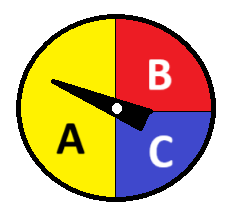
\includegraphics[width=0.2\linewidth]{figs/spinner.png}
\end{center}
% \\~\\
You spin the spinner depicted above, and if it lands in the zone A, you win \$14; if it lands in the zone B, you win \$3; and if it lands in the zone C, you lose \$10. What is the expected amount of money you will win? 
\\
\textarmenian{Դուք պտտում եք վերևում պատկերված պտուտակը, և եթե սլաքը հայտնվում է {\rm A} գոտում, ապա հաղթում եք \$14, եթե հայտնվում է {\rm B} գոտում, հաղթում եք \$3, իսկ եթե հայտնվում է {\rm C} գոտում, պարտվում եք \$10: Որքա՞ն է շահելիք գումարի սպասվող չափը (մաթսպասումը)։}
\end{problem}
\medskip


\begin{problem}
Let $X$ be a random variable with the following PDF:
\[
f_X(x) = \begin{cases}
    (x-1)^3, & 1 \le x \le 3 \\
    0, & \text{otherwise}/\textarmenian{հակառակ դեպքում}
\end{cases}
\]
Find the expectation and variance of $X$. 
\\
\textarmenian{Դիցուք $X$-ը տրված խտության ֆունկցիայով պատահական մեծություն է։ Գտնել $X$-ի մաթսպասումը և վարիացիան։}
\end{problem}


    %  \begin{center}\begin{large} Homework Problems 6
 \end{large}\end{center}
 \bigskip


\begin{problem}[0.5 points]
There are 1 green, 4 blue and 6 red balls in a box. If we randomly
take out 3 balls, what is the probability that exactly 2 of them have
different colors (e.g. 2 blue, 1 green)?

\end{problem}
\bigskip

\begin{problem}[0.5 points]
    Three babies are given a weekly health check at a clinic, and then returned randomly to their mothers. What is the probability that at least one baby goes to the right mother?
\end{problem}

\bigskip

\begin{problem}[0.5 points]
    There are two strawberry-flavored, three caramel and two chocolate candies in the box. Two candies are randomly drawn from the box. What is the probability that one of them will be strawberry-flavored and the other one caramel or chocolate?
\end{problem}
\bigskip
\begin{problem}[1 point]
Ashot, Anush and Armen can hit the target with one shot with probabilities $0.8$, $0.75$ and $0.6$. They shot at the same time and one of them missed the target. What is the probability that it was Armen?
\end{problem}
\bigskip


\begin{problem}[1 point]
You ask your neighbor to water your flowers while you are on vacation. If the flowers are watered, they have about $0.85$ chance of survival; otherwise, they will only survive with probability $0.2$. You are $90$ percent sure your neighbor will water the flowers, but when you are back, you see the flowers are wilted (didn't survive). What is the probability your neighbor didn't water the flowers? Should you trust her anymore? 
\end{problem}

\bigskip


\begin{problem}[1 point]
In a certain town, 30\% of the people are conservatives, 50\% socialists and 20\% liberals. At the last election, 65\% of conservatives voted, 82\% of socialists and 50\% of liberals. A person from the town is selected at random, and states that she voted at the last election. What is
the probability that she is a socialist?
\end{problem}

\bigskip

\begin{problem}[1 point]
    Rosie has ten coins. Nine of them are ordinary coins with equal chances of coming up Head and Tail when tossed, and the tenth has two Heads.
    
    \begin{enumerate}
        \item[a) ] If she takes one of the coins at random from her pocket, what is the probability that it is the coin
with two Heads?

        \item[b) ] If she tosses the coin and it comes up Heads, what is the probability that it is the coin with two Heads?

        \item[c) ] If she tosses the coin one further time and it comes up Tails, what is the probability that it is one of
the nine ordinary coins?

    \end{enumerate}
\end{problem}
\bigskip
\begin{problem}[1 point]
    The world famous gambler Vardanik (from Parakar) proposes the following game of chance. You roll a fair die. If you roll a 1, then Vardanik pays you \$25. If you roll a 2, 
Vardanik pays you \$5. If you roll a 3, you win nothing. If you roll a 4 or a 5, you must 
pay Vardanik \$10, and if you roll a 6, you must pay Vardanik \$15. Do you want to play? 
\end{problem}
\bigskip
\begin{problem}[1 point]
    You draw one card from a 52-card deck of playing cards. If you pick a heart, you will win 
\$10. If you pick a face card (i.e. Jack, Queen or King), which is not a heart, you win \$8. If you pick any other card, 
you lose \$6. Do you want to play? Approximately how much would you win or lose after playing 1,000,000 times?
\end{problem}
\bigskip
\begin{problem}[1 point]
    Let $X$ be a continuous random variable with PDF
\[
f_X(x) = \begin{cases}
    \frac{3}{x^4},& x \ge 1 \\
    0,& \text{otherwise}
\end{cases}
\]

Find the expectation and variance of $X$.
\end{problem}
\bigskip
\begin{problem}[0.5 points]
    Let $X$ and $Y$ be two continuous random variables with uniform distribution on $(0,2)$. Find the expectation of $X+Y$.
\end{problem}

\bigskip
\begin{problem}[1 point]
    Nare and Arman both go to school at some random time between 9:00 and 9:30.
    
    \begin{enumerate}
        \item[a) ] What is the probability that Arman arrives sooner than Nare?
        
        \item[b) ] If after arriving Arman waits another $5$ minutes after he enters, what is the probability that he meets Nare?
        
    \end{enumerate} 
\end{problem}
\bigskip
\begin{problem}[\textbf{optional, not graded}]
    Let $X$ be a random variable with PDF
    \[
    f_X(x) = \begin{cases}
        ax^5,& 0\le x \le 3 \\
        0,& \text{otherwise}
    \end{cases}
    \]
where $a$ is an unknown constant. Find the value of $a$.
\end{problem}


    %  \begin{center}\begin{large} Homework 3, Linear Algebra, Row Echelon Form, Rank, SLE, Invertability, Span\end{large}\end{center}
 \bigskip

\tableofcontents

% 1
\section{Row Echelon Form, Rank}
\begin{problem}%[2 points]
    Bring the following matrices to the Row Echelon Form and find their ranks:

    \begin{enumerate}
        \item[a) ] $C=\begin{bmatrix}3&-2&1\\6&-4&4\end{bmatrix}$,
        
        \item[b) ] $B=\begin{bmatrix}1&4&-2\\2&8&-4\\3&6&2\end{bmatrix}$,
        
        \item[c) ] $C=\begin{bmatrix}1&2&2&1\\3&2&4&2\\-2&-1&-1&-2\end{bmatrix}$,
        
        \item[d) ] $D=\begin{bmatrix}2&4&1&3&2\\-1&-2&1&0&5\\1&6&2&2&2\\3&6&2&5&1\end{bmatrix}$.
    \end{enumerate}
\end{problem}
% \begin{solution}
%      a) $C=\begin{bmatrix}
% 3 & -2 & 1 \\
% 6 & -4 & 4
%     \end{bmatrix}$,
%     \[
%     \begin{bmatrix}
% 3 & -2 & 1 \\
% 6 & -4 & 4
%     \end{bmatrix}
% \xrightarrow{R_2 -2 R_1}
%     \begin{bmatrix}
% 3 & -2 & 1 \\
% 0 & 0 & 2
%     \end{bmatrix}
%     \]
% To bring the matrix to REF it is sufficient to only multiply the first row by $\frac{1}{3}$ and the second row by $\frac{1}{2}$, but we can already say that because there are 2 leading non-zero entries, $\text{rank}(C)=2$.

% For the rest, the technique is the same. You can refer to \href{https://matrixcalc.org/slu.html}{this} and/or \href{https://matrix.reshish.com/rankCalculation.php}{this} webpages for checking your results. 
% \end{solution}

% 2
\section{Systems of linear equations}
\begin{problem}%[2 points]
    Solve the following systems of linear equations using matrices:

    \begin{enumerate}
        \item[a) ] $\begin{cases}
            5x-3y=1\\
            2x+y=18
        \end{cases}$
        
        \item[b) ] $\begin{cases}
            x+y-z=4\\
            3x-y+z=2\\
            x-4z=2
        \end{cases}$
        
        \item[c) ] $\begin{cases}
            x+4y+z=0\\
            x-z=0\\
            9y+7z=0
        \end{cases}$
        
        \item[d) ] $\begin{cases}
            x-y+3z=2\\
            4x+2y-z=-3\\
            -2x-4y+7z=7
        \end{cases}$
        
    \end{enumerate}
\end{problem}

% \begin{solution}
%     b) Let $[\:A\:|\:\vb\:] $ be the augmented matrix
%  \[ [\:A\:|\:\vb\:] = \begin{bmatrix}\

%      1&1&-1&\vert&4\\
%      3&-1&1&\vert&2\\
%      1&0&-4&\vert&2
%  \end{bmatrix} \]
%  Bringing it to REF, we get:
%  \[
%  \begin{bmatrix}

%      1&1&-1&\vert&4\\
%      3&-1&1&\vert&2\\
%      1&0&-4&\vert&2
%  \end{bmatrix} 
%  \xrightarrow{R_2-3R_3}
%  \begin{bmatrix}
%      1&1&-1&\vert&4\\
%      0&-1&13&\vert&-4\\
%      1&0&-4&\vert&2
%  \end{bmatrix} 
%  \xrightarrow{R_1+R_2}\]\[
%  \begin{bmatrix}
%      1&0&12&\vert&0\\
%      0&-1&13&\vert&-4\\
%      1&0&-4&\vert&2
%  \end{bmatrix} 
%  \xrightarrow{R_3-R_1}
%  \begin{bmatrix}
%      1&0&12&\vert&0\\
%      0&-1&13&\vert&-4\\
%      0&0&-16&\vert&2
%  \end{bmatrix} 
%  \xrightarrow{(-1)\cdot R_2}\]\[
%  \begin{bmatrix}
%      1&0&12&\vert&0\\
%      0&1&-13&\vert&4\\
%      0&0&-16&\vert&2
%  \end{bmatrix} 
%  \xrightarrow{-\frac{1}{16}\cdot _3}
%  \begin{bmatrix}
%      1&0&12&\vert&0\\
%      0&1&-13&\vert&4\\
%      0&0&1&\vert&-\frac{1}{8}
%  \end{bmatrix} 
%  \]
%  At this point we can either write it in the form of an SLE and solve for $x,y,z$ or, equivalently, proceed to get the Reduced REF:
%  \[
%  \begin{bmatrix}

%      1&0&12&\vert&0\\
%      0&1&-13&\vert&4\\
%      0&0&1&\vert&-\frac{1}{8}
%  \end{bmatrix} 
%  \xrightarrow{R_1-12R_3}
%  \begin{bmatrix}
%      1&0&0&\vert&\frac{3}{2}\\
%      0&1&-13&\vert&4\\
%      0&0&1&\vert&-\frac{1}{8}
%  \end{bmatrix} 
%  \xrightarrow{R_2+13R_3}
%  \begin{bmatrix}
%      1&0&0&\vert&\frac{3}{2}\\
%      0&1&0&\vert&\frac{19}{8}\\
%      0&0&1&\vert&-\frac{1}{8}
%  \end{bmatrix} 
%  \]
%  whence we have: $x=\dfrac{3}{2},\: y=\dfrac{19}{8},\: z=-\dfrac{1}{8}$.

% For the rest, the technique is the same. You can refer to \href{https://matrixcalc.org/slu.html}{this} webpage for checking your results.
% \end{solution}



% \begin{problem}[2 points]
%     Find, if exists, the inverse of the matrix:

%     \begin{enumerate}
%         \item[a) ] $A=\begin{bmatrix}2&4\\0&1\end{bmatrix}$,
        
%         \item[b) ] $B= \begin{bmatrix}
%             2 & 1 & 3 \\ 5 & -7 & 1 \\ 3 & 0 & -6 
%         \end{bmatrix}$,
        
%         \item[c) ] $C=\begin{bmatrix}0&1&1\\2&-1&1\\1&-1&-1\end{bmatrix}$,
        
%         \item[d) ] $D=\begin{bmatrix}-5&0&3&-1\\0&-5&3&-1\\3&3&-5&4\\-1&-1&4&-6\end{bmatrix}$,

%         \item[e) ] $E=\begin{bmatrix}2&1&4&9\\3&2&4&1\\0&1&-4&2\\-4&-1&-12&-16\end{bmatrix}$.
%     \end{enumerate}

% \end{problem}
% \bigskip

\section{Invertability of a matrix}
\begin{problem}%[1 point]
    Find the value of $a$ such that the following matrix is non-invertible:

        \[ \begin{bmatrix}
            -5 & 0 & a \\ 1 & -2 & 3 \\ 6 & -2 & 1 
        \end{bmatrix} \]
\end{problem}
% \begin{solution}
%     First of all, watch \href{https://www.youtube.com/watch?v=uQhTuRlWMxw}{this} fantastic video by 3blue1brown to form intuition. 

%     A matrix is non-invertible (singular) if and only if if does not have full rank (in our case full-rank is 3). So one approach would be to bring it make the matrix REF and see for which values of $a$ we have that $\text{rank}(a) \neq 3$. Alternatively you can also use the fact that a matrix is non-invertible if and only if it's determinant is zero.

%     Since this whole problem set included REFs and ranks, let's solve this one with determinant approach, so that it's less boring.

%     \[
% \det(\mathbf{A}) = (-5) \det\begin{bmatrix} -2 & 3 \\ -2 & 1 \end{bmatrix} - 
% (0) \det\begin{bmatrix} 1 & 3 \\ 6 & 1 \end{bmatrix} + 
% (a) \det\begin{bmatrix} 1 & -2 \\ 6 & -2 \end{bmatrix}.
% \]
% \[
% \det(\mathbf{A}) = -20 + 10a.  \quad \implies \quad a = 2. \qed
% \]
% \end{solution}

% \bigskip

% \begin{problem}[2 points]
%     Find the eigenvalues and eigenvectors of the following matrices:

%     \begin{enumerate}
%         \item[a) ] $A=\begin{bmatrix}
%             1&2\\0&1\end{bmatrix}$,

%         \item[b) ] $B=\begin{bmatrix}
%             2&1\\1&2
%         \end{bmatrix}$,
        
%         \item[c) ] $C=\begin{bmatrix}
%             6&6&-12\\4&2&-6\\4&3&-7
%         \end{bmatrix}$,
        
%         \item[d) ] $D=\begin{bmatrix}
% -1&0&0\\0&-1&0\\0&0&3        \end{bmatrix}$.
%     \end{enumerate}

%     What are the algebraic and geometric multiplicities of the found eigenvalues?
% \end{problem}

% \bigskip

% \begin{problem}[1 point]
%     Are the following matrices positive definite?

%     \begin{enumerate}
%         \item[a) ] $A=\begin{bmatrix}
%             2&-1&0\\-1&2&-1\\0&-1&2
%         \end{bmatrix}$,

%         \item[b) ] $B=\begin{bmatrix}
%             5&1&1\\1&5&1\\1&1&-2
%         \end{bmatrix}$,

%         \item[c) ] $C=\begin{bmatrix}
%             3&1&2\\1&2&9\\2&2&0
%         \end{bmatrix}$.
%     \end{enumerate}
% \end{problem}


% 4
\section{Dimension of a span}
\begin{problem}%[\textbf{optional, not graded}]
    Find the dimension of the spans of the following vectors:

    \begin{enumerate}
        \item[a) ] $\vv_1=\begin{bmatrix}6\\1\\5\end{bmatrix},  \vv_2=\begin{bmatrix}
            2\\3\\2
        \end{bmatrix}$,

        
        \item[b) ] $\vv_1=\begin{bmatrix}6\\2\end{bmatrix},  \vv_2=\begin{bmatrix}
            1\\3
        \end{bmatrix},  \vv_3=\begin{bmatrix}
            5\\2
        \end{bmatrix}$,
        
        \item[c) ] $\vv_1=\begin{bmatrix}4\\1\\2\end{bmatrix},  \vv_2=\begin{bmatrix}
            -4\\2\\-1
        \end{bmatrix},  \vv_3=\begin{bmatrix}
            8\\-1\\7
        \end{bmatrix}$,
        
        \item[d) ] $\vv_1=\begin{bmatrix}3\\-2\\1\end{bmatrix},  \vv_2=\begin{bmatrix}
            6\\-4\\4
        \end{bmatrix}$.
        
    \end{enumerate}
\end{problem}
% \begin{solution}
%     To find the dimension of the span of a set of vectors, we calculate the \textbf{rank} of the matrix formed by stacking these vectors as columns. The rank corresponds to the number of linearly independent vectors, which is equal to the dimension of the span.

% \begin{enumerate}
%     \item 
%     Form the matrix \(\mathbf{A}\) by placing the vectors as columns:
%     \[
%     \mathbf{A} = \begin{bmatrix}
%        6 & 2 \\
%        1 & 3 \\
%        5 & 2
%     \end{bmatrix}.
%     \]

%     \item From this point this is the same exercise as the first one :)
% \end{enumerate}
% \end{solution}

    %  \begin{center}\begin{large} Practice Problems 2
 \end{large}\end{center}
 \bigskip

% \documentclass{article}
% \usepackage{amsmath}

% \begin{document}


% \begin{problem}
%     Find the trace and determinant of the following matrices:

%     \begin{enumerate}
%         \item[a) ] $A=\begin{bmatrix}
%         2&-1\\-2&-5   \end{bmatrix}$,
        
%         \item[b) ] $B=\begin{bmatrix}
%         4&10\\34&0   \end{bmatrix}$,
        
%         \item[c) ]  $C=\begin{bmatrix}
%         2&6&3\\9&-1&4\\1&5&-2   \end{bmatrix}$,

        
%         \item[d) ]  $D=\begin{bmatrix}
%         5&-1&2\\3&1&-1\\-1&-1&-1   \end{bmatrix}$,
        
%         \item[e) ] $E=\begin{bmatrix}
%         2&0&2&4\\2&0&2&5\\2&0&2&6\\-2&0&-2&-7  \end{bmatrix}$.
%     \end{enumerate}
% \end{problem}
% \bigskip

% \begin{problem}
%     Find the inverse matrix:
%     \begin{enumerate}
%         \item[a) ] $A=\begin{bmatrix}
%         4&3\\5&-1   \end{bmatrix}$,

%         \item[b) ] $B=\begin{bmatrix}
%         7&10\\-3&2   \end{bmatrix}$.
%     \end{enumerate}
% \end{problem}
% \bigskip
% % % \bigskip
% % \newpage

% \begin{center}
%      \begin{large}
%          Solutions
%      \end{large}
%  \end{center}

%  \bigskip



%  \begin{solution} b)

%      \[ 5\va - 10\vb = 5\cdot (\va-2\vb) = 5\cdot \bigg( \begin{bmatrix} 17 \\ 24 \end{bmatrix}-2\cdot\begin{bmatrix} 5 \\ 12 \end{bmatrix} \bigg) =5\cdot \begin{bmatrix} 17-2\cdot 5 \\ 24-2\cdot 12 \end{bmatrix}=5\cdot \begin{bmatrix} 7 \\ 0 \end{bmatrix} =\begin{bmatrix} 35 \\ 0 \end{bmatrix} \]
%  \end{solution}

% \begin{solution} b)
%      \[ \vx \cdot \vy = -(\vx\cdot\vx) = -(2\cdot2+7\cdot 7 + 3\cdot 3) = -62 \]
%  \end{solution}

% \begin{solution}
%  b) $ \va \cdot \vb$ shows the area of lawn mowed by Michael, in square feet,

% c) $0.5 \va \cdot \vb.$
% \end{solution}

% \begin{solution} 
% \begin{enumerate}
%      \item[a) ]  $A = \Z$ is not a vector space; for example, $1 \in B$ but for the scalar $c=0.2$, $c \cdot 1 = 0.2 \not\in B$,
%      \item[b) ]  $B$ is a vector space (check the axioms),
%      \item[c) ]  $C$ is not a vector space, as the axiom 7 does not hold:
%  \[ c\cdot\bigg( \begin{bmatrix} x_1 \\ x_2\end{bmatrix} +  \begin{bmatrix} y_1 \\ y_2\end{bmatrix}\bigg) \neq c \cdot  \begin{bmatrix} x_1 \\ x_2\end{bmatrix}  + c \cdot  \begin{bmatrix} y_1 \\ y_2\end{bmatrix}.  \]
%      \item[d) ]  $D$ is a vector space (check the axioms).
%  \end{enumerate}

%  \end{solution}

% % % 4
%  \begin{solution} b)

%      \[ \va+\vb = \begin{bmatrix} 12-1 \\ 5+2 \\ 0-2 \end{bmatrix} = \begin{bmatrix} 11\\ 7 \\ -2 \end{bmatrix} \]
%  \[ \|\va+\vb\|_1 = |11|+|7|+|-2|=11+7+2=20  \]
%  \[ \|\va+\vb\|_2 = \sqrt{11^2+7^2+(-2)^2}=\sqrt{174}  \]

%  c)

%     \[ \|\vc\|_1 = |3|+|4|=7  \]
%     \[ \|13\vc\|_1 = 13\cdot \|\vc\|_1 = 13\cdot7=91  \]
%     \smallskip
%     \[ \|\vc\|_2 = \sqrt{3^2+4^2}=5  \]
%     \[ \|13\vc\|_2 = 13\cdot \|\vc\|_2 = 13\cdot 5=65  \]
%  \end{solution}
%  \medskip
%  \begin{solution} b) Let $\alpha$ be the angle between $\va$ and $\vb$. Then,

%  \[\cos{\alpha} = \frac{\va\cdot \vb}{\|\va\|\cdot\|\vb\|} = \frac{3 \cdot 3 + 3 \cdot 0}{\sqrt{3^2 + 0^2}\cdot \sqrt{3^2 + 3^2}} = \frac{9}{3\cdot 3\sqrt{2}} = \frac{1}{ \sqrt{2}} \]

%  \[\alpha = \arccos\frac{1}{ \sqrt{2}} = 45^{\circ}.\]
%  \end{solution}
%  \begin{solution} c) 

%  \[A - B = \begin{bmatrix}
%          2-2&5-1&4-5\\-3-(-5)&-2-2&4-2\\5-1&9-6&2-(-1)   \end{bmatrix}
%          = \begin{bmatrix}
%          0&4&-1\\2&-4&2\\4&3&3   \end{bmatrix}
%          \]

%  \begin{align*}
%      (A-&B)C=\begin{bmatrix}
%          0&4&-1\\2&-4&2\\4&3&3   \end{bmatrix} \begin{bmatrix}
%          4&-1\\1&2\\3&3   \end{bmatrix} \\&= \begin{bmatrix}
%          (0 \cdot 4 + 4 \cdot1+(-1) \cdot3) &  (0  \cdot (-1) + 4  \cdot 2 + (-1)  \cdot 3 \\
%          (2 \cdot 4 + (-4) \cdot1+2 \cdot3) &  (2  \cdot (-1) + (-4)  \cdot 2 + 2  \cdot 3 \\
%             (4 \cdot 4 + 3 \cdot1+3 \cdot3) &  (4 \cdot (-1) + 3  \cdot 2 + 3  \cdot 3 \end{bmatrix}
%             = \begin{bmatrix}
%          1&  5\\
%          10& -4 \\
%             28& 11\end{bmatrix}
%  \end{align*}
        
%  \end{solution}
%  \medskip
%  \begin{solution} a)

%  \[\text{tr}(A)=\text{tr}\bigg(\begin{bmatrix}
%          7&-1&5\\6&8&0\\10&2&-6   \end{bmatrix}\bigg) = 7+8+(-6)=9\]

%      b)

%  \[\text{det}(A)=\begin{vmatrix} 7&4\\-3&-4  \end{vmatrix}=7\cdot (-4) - 4\cdot(-3)=-28+12=-16\]


%      d) Using the cofactor method on the 4th column,

%  \begin{align*}
%      \text{det}(A)=\begin{vmatrix} 7&2&4&0\\1&5&0&0\\4&2&0&1\\-2&3&1&2  \end{vmatrix}&=0\cdot (-1)^{1+4}\cdot\begin{vmatrix} 1&5&0\\4&2&0\\-2&3&1  \end{vmatrix}  + 0\cdot (-1)^{2+4}\cdot\begin{vmatrix} 7&2&4\\4&2&0\\-2&3&1 \end{vmatrix}\\&  + 1\cdot (-1)^{3+4}\cdot\begin{vmatrix} 7&2&4\\1&5&0\\-2&3&1 \end{vmatrix} + 2\cdot (-1)^{4+4}\cdot\begin{vmatrix} 7&2&4\\1&5&0\\4&2&0 \end{vmatrix}\\&=-\begin{vmatrix} 7&2&4\\1&5&0\\-2&3&1 \end{vmatrix} +2\cdot\begin{vmatrix} 7&2&4\\1&5&0\\4&2&0 \end{vmatrix}\\&=-85+2\cdot(-72)=-229
%  \end{align*}

%      e) $\det(AB)=\det(A) \cdot \det(B) = \det(A) \cdot 0 = 0.$

%  \end{solution}

%  \begin{solution}
%      b)
%      \[ \det(A) = \begin{vmatrix}
%          7&10\\-3&2
%      \end{vmatrix} = 7\cdot 2 - 10\cdot(-3) = 14 + 30 = 44 \ne 0 \]
%      Therefore, $A$ is invertible and
%      \[ A^{-1} = \frac{1}{44}\begin{bmatrix}
%          2&-10\\3&7
%      \end{bmatrix} \]
%  \end{solution}


\begin{problem}%[2 points]
    Bring the following matrices to the Row Echelon Form and find their ranks:

    \begin{enumerate}
        \item[a) ] $A=\begin{bmatrix}6&2\\1&3\\5&2\end{bmatrix}$,
        
        \item[b) ] $B=\begin{bmatrix}4&1&2\\-4&2&-1\\8&-1&7\end{bmatrix}$,
        
        \item[c) ] $C=\begin{bmatrix}3&-2&1\\6&-4&4\end{bmatrix}$.

        \item[d) ] $D=\begin{bmatrix}2&1&4&9\\3&2&4&1\\0&1&-4&2\\-4&-1&-12&-16\end{bmatrix}$,
        
    \end{enumerate}
\end{problem}

\bigskip


\begin{problem}
    Check whether the vectors $\vv_1, \vv_2, \vv_3$ are linearly independent if:

    \begin{enumerate}
        \item[a) ] $\vv_1=\begin{bmatrix}
            1 \\ 4 \\ 2
        \end{bmatrix}, \vv_2=\begin{bmatrix}
            3 \\ 5 \\ 1
        \end{bmatrix}, \vv_3=\begin{bmatrix}
            1 \\ -3 \\ -3
        \end{bmatrix}, 
        $
        
        \item[b) ] $\vv_1=\begin{bmatrix}
            2 \\ 1 \\ -2
        \end{bmatrix}, \vv_2=\begin{bmatrix}
            3 \\ 2 \\ 0
        \end{bmatrix}, \vv_3=\begin{bmatrix}
            0 \\ 1 \\ 3
        \end{bmatrix}.
        $
        
    \end{enumerate}
\end{problem}

\bigskip 
% \newpage
\begin{problem}
    Solve the following systems of linear equations:

    \begin{enumerate}
        \item[a) ] $\begin{cases}
            3x-y=4\\
            2x+5y=-3
        \end{cases}$
        
        \item[b) ] $\begin{cases}
            x+y-z=4\\
            3x-y+z=2\\
            x-4z=2
        \end{cases}$
        
        \item[c) ] $\begin{cases}
            2x-y+z=5\\
            4x-3y=9\\
            2x-2y-z=4\\
        \end{cases}$
        
    \end{enumerate}
\end{problem}
\bigskip

% \begin{problem}
%     Find, if exists, the inverse of the matrix:

%     \begin{enumerate}
%         \item[a) ] $A=\begin{bmatrix}1&-1\\0&2\end{bmatrix}$,
        
%         \item[b) ] $B=\begin{bmatrix}1&-1&1\\2&3&0\\0&-2&1\end{bmatrix}$,
        
%         \item[c) ] $C=\begin{bmatrix}2&3&1\\3&3&1\\2&4&1\end{bmatrix}$,
        
%         \item[d) ] $D=\begin{bmatrix}2&-17&11\\-1&11&-7\\0&3&-2\end{bmatrix}$.
%     \end{enumerate}
% \end{problem}
% \bigskip

% \begin{problem}
%     Find the eigenvalues and eigenvectors of the following matrices:

%     \begin{enumerate}
%         \item[a) ] $A=\begin{bmatrix}
%             -5&2\\-7&4
%         \end{bmatrix}$,
        
%         \item[b) ] $B=\begin{bmatrix}
%             1&0\\0&1
%         \end{bmatrix}$,
        
        
%         \item[c) ] $C=\begin{bmatrix}
%             2&2&-2\\1&3&-1\\-1&1&1
%         \end{bmatrix}$,
%     \end{enumerate}

%     What are the algebraic and geometric multiplicities of the found eigenvalues?
% \end{problem}

% % \bigskip


 \newpage



\begin{solution}
    c) $C=\begin{bmatrix}
3 & -2 & 1 \\
6 & -4 & 4
    \end{bmatrix}$,
    \[
    \begin{bmatrix}
3 & -2 & 1 \\
6 & -4 & 4
    \end{bmatrix}
\xrightarrow{R_2 -2 R_1}
    \begin{bmatrix}
3 & -2 & 1 \\
0 & 0 & 2
    \end{bmatrix}
    \]
To bring the matrix to REF it is sufficient to only multiply the first row by $\frac{1}{3}$ and the second row by $\frac{1}{2}$, but we can already say that because there are 2 leading non-zero entries, $\text{rank}(C)=2$.

    
\end{solution}
\bigskip

\begin{solution}
b) To check if a set of vectors is linearly independent or not, we can put together those vectors as rows or columns of a matrix and find its rank. For example, 
\[B=
\begin{bmatrix}
     \vv_1^T \\ \vv_2^T \\ \vv_3^T
\end{bmatrix}
 =
 \begin{bmatrix}
     2 & 1 & -2 \\
     3 & 2 & 0 \\
     0 & 1 & 3
 \end{bmatrix}
 \xrightarrow{R_2 -1.5 R_1}
 \begin{bmatrix}
     2 & 1 & -2 \\
     0 & -0.5 & 3 \\
     0 & 1 & 3
 \end{bmatrix}
 \xrightarrow[R_3 + 2R_2]{R_1+2R_2}
 \begin{bmatrix}
     2 & 0 & 4 \\
     0 & -0.5 & 3 \\
     0 & 0 & 9
 \end{bmatrix}
 \]

 Again, multiplying each row with a corresponding number will result in 3 leading ones, therefore $\operatorname{rank}(B)=3$ which simply means that its rows, $\vv_1,\vv_2,$ and $\vv_3$, are linearly independent.

 \end{solution}
 \bigskip

 \begin{solution}
 b) Let $[\:A\:|\:\vb\:] $ be the augmented matrix
 \[ [\:A\:|\:\vb\:] = \begin{bmatrix}\

     1&1&-1&\vert&4\\
     3&-1&1&\vert&2\\
     1&0&-4&\vert&2
 \end{bmatrix} \]
 Bringing it to REF, we get:
 \[
 \begin{bmatrix}

     1&1&-1&\vert&4\\
     3&-1&1&\vert&2\\
     1&0&-4&\vert&2
 \end{bmatrix} 
 \xrightarrow{R_2-3R_3}
 \begin{bmatrix}
     1&1&-1&\vert&4\\
     0&-1&13&\vert&-4\\
     1&0&-4&\vert&2
 \end{bmatrix} 
 \xrightarrow{R_1+R_2}\]\[
 \begin{bmatrix}
     1&0&12&\vert&0\\
     0&-1&13&\vert&-4\\
     1&0&-4&\vert&2
 \end{bmatrix} 
 \xrightarrow{R_3-R_1}
 \begin{bmatrix}
     1&0&12&\vert&0\\
     0&-1&13&\vert&-4\\
     0&0&-16&\vert&2
 \end{bmatrix} 
 \xrightarrow{(-1)\cdot R_2}\]\[
 \begin{bmatrix}
     1&0&12&\vert&0\\
     0&1&-13&\vert&4\\
     0&0&-16&\vert&2
 \end{bmatrix} 
 \xrightarrow{-\frac{1}{16}\cdot _3}
 \begin{bmatrix}
     1&0&12&\vert&0\\
     0&1&-13&\vert&4\\
     0&0&1&\vert&-\frac{1}{8}
 \end{bmatrix} 
 \]
 At this point we can either write it in the form of an SLE and solve for $x,y,z$ or, equivalently, proceed to get the Reduced REF:
 \[
 \begin{bmatrix}

     1&0&12&\vert&0\\
     0&1&-13&\vert&4\\
     0&0&1&\vert&-\frac{1}{8}
 \end{bmatrix} 
 \xrightarrow{R_1-12R_3}
 \begin{bmatrix}
     1&0&0&\vert&\frac{3}{2}\\
     0&1&-13&\vert&4\\
     0&0&1&\vert&-\frac{1}{8}
 \end{bmatrix} 
 \xrightarrow{R_2+13R_3}
 \begin{bmatrix}
     1&0&0&\vert&\frac{3}{2}\\
     0&1&0&\vert&\frac{19}{8}\\
     0&0&1&\vert&-\frac{1}{8}
 \end{bmatrix} 
 \]
 whence we have: $x=\dfrac{3}{2},\: y=\dfrac{19}{8},\: z=-\dfrac{1}{8}$.
 \end{solution}

 \bigskip

 \begin{solution}
     c) \[
 \begin{bmatrix}
     2 & 3 & 1 & | & 1 & 0 & 0 \\
     3 & 3 & 1 & | & 0 & 1 & 0 \\
     2 & 4 & 1 & | & 0 & 0 & 1 \\
 \end{bmatrix} \xrightarrow{R_1\leftrightarrow R_2} \begin{bmatrix}
     3 & 3 & 1 & | & 0 & 1 & 0 \\
     2 & 3 & 1 & | & 1 & 0 & 0 \\
     2 & 4 & 1 & | & 0 & 0 & 1 \\
 \end{bmatrix} \xrightarrow{R_1- R_2}
 \begin{bmatrix}
     1 & 0 & 0 & | & -1 & 1 & 0 \\
     2 & 3 & 1 & | & 1 & 0 & 0 \\
     2 & 4 & 1 & | & 0 & 0 & 1 \\
 \end{bmatrix}
 \]
 \[
 \xrightarrow{R_3- R_2}\begin{bmatrix}
     1 & 0 & 0 & | & -1 & 1 & 0 \\
     2 & 3 & 1 & | & 1 & 0 & 0 \\
     0 & 1 & 0 & | & -1 & 0 & 1 \\
 \end{bmatrix}\xrightarrow{R_3 \leftrightarrow R_2}
 \begin{bmatrix}
     1 & 0 & 0 & | & -1 & 1 & 0 \\  
     0 & 1 & 0 & | & -1 & 0 & 1 \\
     2 & 3 & 1 & | & 1 & 0 & 0 \\
    
 \end{bmatrix}\]\[\xrightarrow{R_3 -2 R_1}
 \begin{bmatrix}
     1 & 0 & 0 & | & -1 & 1 & 0 \\  
     0 & 1 & 0 & | & -1 & 0 & 1 \\
     0 & 3 & 1 & | & 3 & -2 & 0 \\    
 \end{bmatrix}\xrightarrow{R_3 -3 R_2}
 \begin{bmatrix}
     1 & 0 & 0 & | & -1 & 1 & 0 \\  
     0 & 1 & 0 & | & -1 & 0 & 1 \\
     0 & 0 & 1 & | & 6 & -2 & -3 \\    
 \end{bmatrix}%=[\:I\:|\:A^{-1}\:]
 \]

 Thus,
 \[ C^{-1} = \begin{bmatrix} -1 & 1 & 0 \\ -1 & 0 & 1 \\ 6 &-2 & -3 \end{bmatrix} \]

 \end{solution}

 \bigskip
 \begin{solution}
     a) $A=\begin{bmatrix}
             -5&2\\-7&4
         \end{bmatrix}$,
        
        
         We write its characteristic polynomial to find the eigenvalues:
         \[  \det(A-\lambda I)=\left|\begin{array}{cc}
             -5-\lambda&2\\-7&4-\lambda
         \end{array}\right| =\lambda^2+\lambda-6=(\lambda+3)(\lambda-2)=0, \]
         hence both roots $\lambda = -3$ and $\lambda = 2$ have algebraic multiplicities of $1$.
         \begin{itemize}
             \item To find the eigenvectors $\vv=\begin{bmatrix}
             v_1\\v_2
         \end{bmatrix}\ne \textbf{0}$ corresponding to $\lambda = -3$, we let:
         \[
         A\vv=-3 \vv
         \]
         \[
         \begin{bmatrix}
             -5v_1 + 2v_2 \\ -7v_1 + 4v_2
         \end{bmatrix} = \begin{bmatrix}
             -3v_1 \\ -3v_2
         \end{bmatrix}
         \]
         whence we have $v_1=v_2$ (in fact, both equations give the same result). So the eigenvectors are:
         \[
         E_{-3} = \left\{ a \cdot \begin{bmatrix}
             1 \\ 1
         \end{bmatrix} \bigg\vert\: a\in\R \right\}
         \]

         Due to the fact that all vectors in $E_{-3}$ are multiples of only one vector $\begin{bmatrix}
             1 \\ 1
         \end{bmatrix}$, we see that $\dim(E_{-3})=1$, so $\lambda=-3$ has geometric multiplicity of $1$.

        
             \item To find the eigenvectors corresponding to $\lambda = 2$, we let:
         \[
         A\vv=2 \vv
         \]
         \[
         \begin{bmatrix}
             -5v_1 + 2v_2 \\ -7v_1 + 4v_2
         \end{bmatrix} = \begin{bmatrix}
             2v_1 \\ 2v_2
         \end{bmatrix}
         \]
         whence $v_1=\frac{2}{7}v_2$ (in fact, both equations give the same result). So the eigenvectors are:
         \[
         E_{2} = \left\{ a \cdot \begin{bmatrix}
             \frac{2}{7} \\ 1
         \end{bmatrix} \bigg\vert\: a\in\R \right\} = \left\{ a \cdot \begin{bmatrix}
             2 \\ 7
         \end{bmatrix} \bigg\vert\: a\in\R \right\}
         \]

         With the same logic, $\dim(E_{2})=1$, so $\lambda=2$ has geometric multiplicity of $1$ too.

         \end{itemize}
        
 \end{solution}
    %\begin{center}\begin{large} Homework 2 Solutions
 \end{large}\end{center}
 \bigskip

% \documentclass{article}
% \usepackage{amsmath}

% \begin{document}


\begin{problem}[3 points]
Check if the following set is a vector space:

    \begin{enumerate}
        \item [a)] The set of real negative numbers $A = \{x\in\R \mid x < 0\}$, with the usual operations $+$ and $\cdot$,

        \item [b)] $B = \left\{ \begin{bmatrix} a \\ b \\ c\end{bmatrix} \mid \text{ for all real numbers }a, b, c\in\R\right\}$, with the usual operation of $\cdot$, and the addition defined as:
        \[ \begin{bmatrix} a_1 \\ b_1 \\ c_1\end{bmatrix} + \begin{bmatrix} a_2 \\ b_2 \\ c_2\end{bmatrix} = \begin{bmatrix} a_1 + a_2 \\ b_1 + b_2\\ c_1 + c_2 - 1\end{bmatrix} ,\]
        
        \item [c)] $C =  \bigg\{ \begin{bmatrix} a \\ b \end{bmatrix} \mid \text{ for all numbers }a,b\in\R\bigg\}$, with the usual operation of $\cdot$, and the addition defined as:
        \[ \begin{bmatrix} a_1 \\ b_1 \end{bmatrix} +\begin{bmatrix} a_2 \\ b_2 \end{bmatrix} = \begin{bmatrix} a_1-a_2 \\ b_1-b_2 \end{bmatrix} , \]

        \item [d)] $D =  \bigg\{ \begin{bmatrix} a \\ b \end{bmatrix} \mid \text{ for all numbers }a,b\in\R\bigg\}$, with the usual operation of $\cdot$, and the addition defined as:
        \[ \begin{bmatrix} a_1 \\ b_1 \end{bmatrix} +\begin{bmatrix} a_2 \\ b_2 \end{bmatrix} = \begin{bmatrix} 0 \\ 0\end{bmatrix}  ,\]
        
        \item [e)] $E =  \bigg\{ \begin{bmatrix} a \\ b \end{bmatrix} \mid \text{ for all numbers }a,b\in\R\bigg\}$, with the usual operation of $+$, and the scalar multiplication defined as:
        \[ c \cdot \begin{bmatrix} a \\ b \end{bmatrix} = \begin{bmatrix} c \cdot ( a+b) \\ cb\end{bmatrix}  , \qquad \text{for any } c>0.\]

        \item [f)] The set of all polynomials of degree $2$, with the usual operations $+$ and $\cdot$.

        
    \end{enumerate}
\end{problem}

\begin{sol}
    \begin{enumerate}
    {
        \item [a)]
    To determine if the set \( A = \{ x \in \mathbb{R} \mid x < 0 \} \) is a vector space, we need to verify if it satisfies all the vector space axioms under the usual operations of addition \( + \) and scalar multiplication \( \cdot \).

    First of all, the following 2 properties should hold:
    \begin{itemize}
        \item \textbf{Closure under addition}: For any \( x, y \in A \), \( x + y \) should also be in \( A \).
        
        \item \textbf{Closure under scalar multiplication}: For any \( x \in A \) and any scalar \( c \in \mathbb{R} \), \( c \cdot x \) should also be in \( A \).
    \end{itemize}

    Let's check.

    \begin{enumerate}
        \item \textbf{Closure under addition}: Let \( x, y \in A \), meaning \( x < 0 \) and \( y < 0 \). Then \( x + y < 0 \) (since the sum of two negative numbers is also negative). Therefore, \( x + y \in A \), so \( A \) is closed under addition.

        \item \textbf{Closure under scalar multiplication}: For \( x \in A \) and any scalar \( c \in \mathbb{R} \):
        
        - If \( c > 0 \), then \( c \cdot x < 0 \) since \( x < 0 \). \\
        - If \( c < 0 \), then \( c \cdot x > 0 \), which is not in \( A \). \\
        - If \( c = 0 \), then \( c \cdot x = 0 \), which is also not in \( A \) (since \( 0 \not< 0 \)).

        Thus, \( A \) is not closed under scalar multiplication.
    \end{enumerate}
    No need to do anything else, showing that something is \textbf{not} a vector space is much more pleasant because we can just stop after one axiom breaks. On the other hand, if it is a vector space than we must check every axiom.
    }

    \item[b)] ToDo
    \item[c)] ToDo
    \item[d)] ToDo
    \item[e)] ToDo
    \item[f)] ToDo
    
    \end{enumerate}
    
\end{sol}

\newpage

\begin{problem}[2 point]
    Calculate the Manhattan (L1) and Euclidean (L2) norms of the following vectors:

    \begin{enumerate}
        \item[a) ] $\va= \begin{bmatrix} 2\\-9\\3 \end{bmatrix}$,
        
        \item[b) ] $\va-2\vb$, where $\va= \begin{bmatrix}3\\4\\1\\0\end{bmatrix}, \vb = \begin{bmatrix}4\\5\\-2\\-1\end{bmatrix}$,
        
        \item[c) ] $-3\vc$, where $\vc= \begin{bmatrix}2\\-5\\6\end{bmatrix}$.
    \end{enumerate}
    % \bigskip

    %     \textbf{Optional, not graded}: Find the angle between $\va$ in \textit{a)} and $\vc$ in \textit{c)}.
\end{problem}

% 2
\begin{sol}
   Let's first recall the definitions:

    For a vector $\vx = \begin{bmatrix} x_1 & x_2 & \dots & x_n \end{bmatrix}^\top$

    - \textbf{Manhattan (L1) norm}: 
      \[
      \|\vx\|_1 = |x_1| + |x_2| + \dots + |x_n|
      \]
      
    - \textbf{Euclidean (L2) norm}: 
      \[
      \|\vx\|_2 = \sqrt{x_1^2 + x_2^2 + \dots + x_n^2}
      \]
      
    Now let's get to work:

    \begin{enumerate}
        \item[a)] For $\va= \begin{bmatrix} 2 \\ -9 \\ 3 \end{bmatrix}$:
        
        \[
        \|\va\|_1 = |2| + |-9| + |3| = 2 + 9 + 3 = 14
        \]
        
        \[
        \|\va\|_2 = \sqrt{2^2 + (-9)^2 + 3^2} = \sqrt{4 + 81 + 9} = \sqrt{94}
        \]
        
        \item[b)] For $\va - 2\vb$, where $\va= \begin{bmatrix} 3 \\ 4 \\ 1 \\ 0 \end{bmatrix}$ and $\vb = \begin{bmatrix} 4 \\ 5 \\ -2 \\ -1 \end{bmatrix}$:
        
        First, compute $\va - 2\vb$:
        
        \[
        \va - 2\vb = \begin{bmatrix} 3 \\ 4 \\ 1 \\ 0 \end{bmatrix} - 2 \cdot \begin{bmatrix} 4 \\ 5 \\ -2 \\ -1 \end{bmatrix} = \begin{bmatrix} 3 \\ 4 \\ 1 \\ 0 \end{bmatrix} - \begin{bmatrix} 8 \\ 10 \\ -4 \\ -2 \end{bmatrix} = \begin{bmatrix} -5 \\ -6 \\ 5 \\ 2 \end{bmatrix}
        \]
        
        Now calculate the norms:
        
        \[
        \|\va - 2\vb\|_1 = |-5| + |-6| + |5| + |2| = 5 + 6 + 5 + 2 = 18
        \]
        
        \[
        \|\va - 2\vb\|_2 = \sqrt{(-5)^2 + (-6)^2 + 5^2 + 2^2} = \sqrt{25 + 36 + 25 + 4} = \sqrt{90}
        \]
        
        \item[c)] For $-3\vc$, where $\vc= \begin{bmatrix} 2 \\ -5 \\ 6 \end{bmatrix}$:
        
        First, compute $-3\vc$:
        
        \[
        -3\vc = -3 \cdot \begin{bmatrix} 2 \\ -5 \\ 6 \end{bmatrix} = \begin{bmatrix} -6 \\ 15 \\ -18 \end{bmatrix}
        \]
        
        Now calculate the norms:
        
        \[
        \|-3\vc\|_1 = |-6| + |15| + |-18| = 6 + 15 + 18 = 39
        \]
        
        \[
        \|-3\vc\|_2 = \sqrt{(-6)^2 + 15^2 + (-18)^2} = \sqrt{36 + 225 + 324} = \sqrt{585}
        \]
    \end{enumerate}

    Thus, the solutions are:
    
    \begin{enumerate}
        \item[a)] $\|\va\|_1 = 14$, \quad $\|\va\|_2 = \sqrt{94}$
        \item[b)] $\|\va - 2\vb\|_1 = 18$, \quad $\|\va - 2\vb\|_2 = \sqrt{90}$
        \item[c)] $\|-3\vc\|_1 = 39$, \quad $\|-3\vc\|_2 = \sqrt{585}$
    \end{enumerate}
\end{sol}

\newpage

% 3
\begin{problem}[1 point]
    Find the angles between the following vectors:

    \begin{enumerate}
        \item[a) ] $\va= \begin{bmatrix} 2\\1\\1\end{bmatrix}$ and $\vb= \begin{bmatrix} 1\\-3\\3\end{bmatrix}$,
        
        \item[b) ] The vectors $\va$ and $\vc$ in Problem 2a and 2c.

    \end{enumerate}
\end{problem}
\bigskip

\begin{sol}
    To find the angle $\theta$ between two vectors $\va$ and $\vb$, we use the following formula:

    \[
    \cos \theta = \frac{\va \cdot \vb}{\|\va\| \|\vb\|}
    \]

    where $\va \cdot \vb$ is the dot product of $\va$ and $\vb$, and $\|\va\|$ and $\|\vb\|$ are the magnitudes (lengths) (Euclidean norms) of $\va$ and $\vb$.

    \begin{enumerate}
        \item[a)] For $\va= \begin{bmatrix} 2 \\ 1 \\ 1 \end{bmatrix}$ and $\vb= \begin{bmatrix} 1 \\ -3 \\ 3 \end{bmatrix}$:

        - First, compute the dot product $\va \cdot \vb$:
          \[
          \va \cdot \vb = 2 \cdot 1 + 1 \cdot (-3) + 1 \cdot 3 = 2 - 3 + 3 = 2
          \]

        - Next, compute the magnitudes (lengths) $\|\va\|$ and $\|\vb\|$:
          \[
          \|\va\| = \sqrt{2^2 + 1^2 + 1^2} = \sqrt{4 + 1 + 1} = \sqrt{6}
          \]
          \[
          \|\vb\| = \sqrt{1^2 + (-3)^2 + 3^2} = \sqrt{1 + 9 + 9} = \sqrt{19}
          \]

        - Now we can find $\cos \theta$:
          \[
          \cos \theta = \frac{\va \cdot \vb}{\|\va\| \|\vb\|} = \frac{2}{\sqrt{6} \cdot \sqrt{19}} = \frac{2}{\sqrt{114}}
          \]

        - Therefore, the angle $\theta$ between $\va$ and $\vb$ is:
          \[
          \theta = \cos^{-1} \left( \frac{2}{\sqrt{114}} \right)
          \]

        - We don't really care about the actual value of such an unpleasant number, but if you're curious, the answer is approximately 79.2 degrees.

        \item[b)] For vectors $\va$ and $\vc$ from Problem 2a and 2c, where $\va= \begin{bmatrix} 2 \\ -9 \\ 3 \end{bmatrix}$ and $\vc = \begin{bmatrix} 2 \\ -5 \\ 6 \end{bmatrix}$:

        - First, compute the dot product $\va \cdot \vc$:
          \[
          \va \cdot \vc = 2 \cdot 2 + (-9) \cdot (-5) + 3 \cdot 6 = 4 + 45 + 18 = 67
          \]

        - Next, compute the magnitudes $\|\va\|$ and $\|\vc\|$:
          \[
          \|\va\| = \sqrt{2^2 + (-9)^2 + 3^2} = \sqrt{4 + 81 + 9} = \sqrt{94}
          \]
          \[
          \|\vc\| = \sqrt{2^2 + (-5)^2 + 6^2} = \sqrt{4 + 25 + 36} = \sqrt{65}
          \]

        - Now we can find $\cos \theta$:
          \[
          \cos \theta = \frac{\va \cdot \vc}{\|\va\| \|\vc\|} = \frac{67}{\sqrt{94} \cdot \sqrt{65}} = \frac{67}{\sqrt{6110}}
          \]

        - Therefore, the angle $\theta$ between $\va$ and $\vc$ is:
          \[
          \theta = \cos^{-1} \left( \frac{67}{\sqrt{6110}} \right)
          \] 
    \end{enumerate}
\end{sol}



% \begin{problem}[1 point]
%     Given the following system of equations, find values for $a$ and $b$:
%    \[ \begin{cases}
%          a + 3b = 4 \\
%          a - b = -4 
%     \end{cases}\]

%     How can we write the equations in terms of matrices?
% \end{problem}


\newpage
% 4
\begin{problem}[2 points]
    Evaluate the expression:

    \begin{enumerate}
        \item[a) ] $AB$, where $A=\begin{bmatrix}
        6&5\\-2&7  \end{bmatrix}$, $B=\begin{bmatrix}
        -5&3\\1&4   \end{bmatrix}$,

        \item[b) ] $B^3$, where $B=\begin{bmatrix}
        -2&1&4\\1&2&1\\-2&-2&0   \end{bmatrix}$,

        \item[c) ] $CD$, where $C=\begin{bmatrix}
        7&2&-3\\0&2&8\\8&1&-3\\4&3&-1   \end{bmatrix}$, $D=\begin{bmatrix}
            -2&4\\8&1\\-1&5
        \end{bmatrix}$,
        
        \item[d) ] $(A-B)(A+B)$, where $A=\begin{bmatrix}
        2&2&4\\-3&-2&4\\-2&0&2   \end{bmatrix}$, $B=\begin{bmatrix}
        2&1&3\\-1&2&2\\1&4&-1   \end{bmatrix}$,
        
        \item[e) ] $A^2 - B^2$, with the same $A$ and $B$ as in \textit{d)}.
    \end{enumerate}
\end{problem}

\begin{sol}
    This is a super boring exercise, but everyone needs to go through this suffering at least once to get familiar with the pain of multiplying matrices. That being said, let's have some fun:
    \begin{enumerate}
        \item[a)] Compute $AB$, where 
        \[
        A = \begin{bmatrix} 6 & 5 \\ -2 & 7 \end{bmatrix}, \quad B = \begin{bmatrix} -5 & 3 \\ 1 & 4 \end{bmatrix}
        \]

          \[
          AB = \begin{bmatrix} 6 \cdot (-5) + 5 \cdot 1 & 6 \cdot 3 + 5 \cdot 4 \\ -2 \cdot (-5) + 7 \cdot 1 & -2 \cdot 3 + 7 \cdot 4 \end{bmatrix}
          \]
          \[
          = \begin{bmatrix} -30 + 5 & 18 + 20 \\ 10 + 7 & -6 + 28 \end{bmatrix} = \begin{bmatrix} -25 & 38 \\ 17 & 22 \end{bmatrix}
          \]

        \item[b)] Compute $B^3$, where 
        \[
        B = \begin{bmatrix} -2 & 1 & 4 \\ 1 & 2 & 1 \\ -2 & -2 & 0 \end{bmatrix}
        \]

        - First, find $B^2 = B \cdot B$ and then multiply the result by $B$ to get $B^3$.
        
        \[
        B^2 = \begin{bmatrix} -2 & 1 & 4 \\ 1 & 2 & 1 \\ -2 & -2 & 0 \end{bmatrix} \cdot \begin{bmatrix} -2 & 1 & 4 \\ 1 & 2 & 1 \\ -2 & -2 & 0 \end{bmatrix}
        \]
        
        - Calculating each entry of $B^2$ yields:
          \[
          B^2 = \begin{bmatrix} -3 & -8 & -7 \\ -2 & 3 & 6 \\ 2 & -6 & -10 \end{bmatrix}
          \]

        - Now, calculate $B^3 = B^2 \cdot B$:
          \[
          B^3 = \begin{bmatrix} -3 & -8 & -7 \\ -2 & 3 & 6 \\ 2 & -6 & -10 \end{bmatrix} \cdot \begin{bmatrix} -2 & 1 & 4 \\ 1 & 2 & 1 \\ -2 & -2 & 0 \end{bmatrix}
          \]
          
          - Calculating each entry of $B^3$ gives:
            \[
            B^3 = \begin{bmatrix} 12 & -5 & -20 \\ -5 & -8 & -5 \\ 10 & 10 & 2 \end{bmatrix}
            \]

        \item[c)] Compute $CD$, where 
        \[
        C = \begin{bmatrix} 7 & 2 & -3 \\ 0 & 2 & 8 \\ 8 & 1 & -3 \\ 4 & 3 & -1 \end{bmatrix}, \quad D = \begin{bmatrix} -2 & 4 \\ 8 & 1 \\ -1 & 5 \end{bmatrix}
        \]
        - Let's note that we can actually perform matrix multiplication because $C$ has dimensions 4x3 and $D$ has dimensions 3x2. If the number of columns of the first matrix matches the number of rows of the second one than we're good to go. We can also note that the result will be a 4 by 2 matrix.  
        
        - Calculate each entry of $CD$:
          \[
          CD = \begin{bmatrix} 7 \cdot (-2) + 2 \cdot 8 + (-3) \cdot (-1) & 7 \cdot 4 + 2 \cdot 1 + (-3) \cdot 5 \\ 0 \cdot (-2) + 2 \cdot 8 + 8 \cdot (-1) & 0 \cdot 4 + 2 \cdot 1 + 8 \cdot 5 \\ 8 \cdot (-2) + 1 \cdot 8 + (-3) \cdot (-1) & 8 \cdot 4 + 1 \cdot 1 + (-3) \cdot 5 \\ 4 \cdot (-2) + 3 \cdot 8 + (-1) \cdot (-1) & 4 \cdot 4 + 3 \cdot 1 + (-1) \cdot 5 \end{bmatrix}
          \]
          
          \[
          = \begin{bmatrix} 5 & 15 \\ 8 & 42 \\ -5 & 18 \\ 17 & 14 \end{bmatrix}
          \]

        \item[d)] Compute $(A - B)(A + B)$, where 
        \[
        A = \begin{bmatrix} 2 & 2 & 4 \\ -3 & -2 & 4 \\ -2 & 0 & 2 \end{bmatrix}, \quad B = \begin{bmatrix} 2 & 1 & 3 \\ -1 & 2 & 2 \\ 1 & 4 & -1 \end{bmatrix}
        \]

        - First, calculate $A - B$ and $A + B$:
          \[
          A - B = \begin{bmatrix} 2 - 2 & 2 - 1 & 4 - 3 \\ -3 - (-1) & -2 - 2 & 4 - 2 \\ -2 - 1 & 0 - 4 & 2 - (-1) \end{bmatrix} = \begin{bmatrix} 0 & 1 & 1 \\ -2 & -4 & 2 \\ -3 & -4 & 3 \end{bmatrix}
          \]
          \[
          A + B = \begin{bmatrix} 2 + 2 & 2 + 1 & 4 + 3 \\ -3 + (-1) & -2 + 2 & 4 + 2 \\ -2 + 1 & 0 + 4 & 2 + (-1) \end{bmatrix} = \begin{bmatrix} 4 & 3 & 7 \\ -4 & 0 & 6 \\ -1 & 4 & 1 \end{bmatrix}
          \]

        - Now calculate $(A - B)(A + B)$:
          \[
          (A - B)(A + B) = \begin{bmatrix} 0 & 1 & 1 \\ -2 & -4 & 2 \\ -3 & -4 & 3 \end{bmatrix} \cdot \begin{bmatrix} 4 & 3 & 7 \\ -4 & 0 & 6 \\ -1 & 4 & 1 \end{bmatrix} 
          = \begin{bmatrix} -5 & 4 & 7 \\ 6 & 2 & -36 \\ 1 & 3 & -42 \end{bmatrix}
          \]
          
          
        \item[e)] Compute $A^2 - B^2$ for the same $A$ and $B$ as in part (d): \\
        \textbf{\textcolor{red}{WAIT!!!!!}}
        Before starting to do this, do you think you can guess what the answer is? Think for a little while, maybe grab a cup of tea. Ready? Okay, let's go.

        - First, calculate $A^2$ and $B^2$ separately:
          \[
          A^2 = A \cdot A = \begin{bmatrix} 2 & 2 & 4 \\ -3 & -2 & 4 \\ -2 & 0 & 2 \end{bmatrix} \cdot \begin{bmatrix} 2 & 2 & 4 \\ -3 & -2 & 4 \\ -2 & 0 & 2 \end{bmatrix} = \begin{bmatrix} -10 & 0 & 24 \\ -8 & -2 & -12 \\ -8 & -4 & -4 \end{bmatrix}
          \]
          \[
          B^2 = B \cdot B = \begin{bmatrix} 2 & 1 & 3 \\ -1 & 2 & 2 \\ 1 & 4 & -1 \end{bmatrix} \cdot \begin{bmatrix} 2 & 1 & 3 \\ -1 & 2 & 2 \\ 1 & 4 & -1 \end{bmatrix} = \begin{bmatrix} 6 & 16 & 5 \\ -2 & 11 & -1 \\ -3 & 5 & 12 \end{bmatrix}
          \]

        - Now calculate $A^2 - B^2$:
          \[
          A^2 - B^2 = \begin{bmatrix} -10 & 0 & 24 \\ -8 & -2 & -12 \\ -8 & -4 & -4 \end{bmatrix} - \begin{bmatrix} 6 & 16 & 5 \\ -2 & 11 & -1 \\ -3 & 5 & 12 \end{bmatrix} = \begin{bmatrix} -16 & -16 & 19 \\ -6 & -13 & -11 \\ -5 & -9 & -16 \end{bmatrix} 
          \]

        So, the answer is not the same as in the previous exercise. Did you guess correctly? Can you figure out what condition should hold for $A$ and $B$ in order for the answer to be the same. Here (https://math.stackexchange.com/questions/3518069/conditions-for-a2-b2-aba-b-to-be-true) is a link that you can refer to, but only after struggling on your own. We want know if you click the link right away, but we hope you won't do it :)
    \end{enumerate}
\end{sol}


\newpage

% 5
\begin{problem}[2 points]
    Evaluate the expression:

    \begin{enumerate}
        \item[a) ] $\det(A)$, where $A=\begin{bmatrix}
        8&3&5\\1&4&2\\-4&0&4   \end{bmatrix}$,

        \item[b) ] $\text{det}(B)-\text{tr}(B)$, where $B=\begin{bmatrix}
        5&2&1\\4&-1&4\\-3&1&2 \end{bmatrix}$,
        
        \item[c) ] $\text{det}(C)$, where $C=\begin{bmatrix}
        3&0&1&3\\2&0&4&1\\0&2&-1&3\\5&0&0&3   \end{bmatrix}$,
        
        \item[d) ] $\text{det}(D)$, where $D=\begin{bmatrix}
        5&2&-3&2\\1&0&4&1\\0&5&0&-2\\1&1&5&-1  \end{bmatrix}$.
    \end{enumerate}
\end{problem}

\begin{sol}
    This is not the most fun exercise as well, but practice is important.
    \begin{enumerate}
        \item[a)] Compute $\det(A)$, where 
        \[
        A = \begin{bmatrix} 8 & 3 & 5 \\ 1 & 4 & 2 \\ -4 & 0 & 4 \end{bmatrix}
        \]

        Using the formula for a 3x3 determinant with six terms (three positive and three negative), we have:
        \[
        \det(A) = 8 \cdot 4 \cdot 4 + 3 \cdot 2 \cdot (-4) + 5 \cdot 1 \cdot 0 - (5 \cdot 4 \cdot (-4) + 3 \cdot 1 \cdot 4 + 8 \cdot 2 \cdot 0)
        \]
        \[
        = 8 \cdot 16 + 3 \cdot (-8) + 0 - (5 \cdot (-16) + 3 \cdot 4 + 0)
        \]
        \[
        = 128 - 24 + 0 - (-80 + 12 + 0) = 128 - 24 + 80 - 12 = 172
        \]

        So, $\det(A) = 172$.

        \item[b)] Compute $\det(B) - \text{tr}(B)$, where 
        \[
        B = \begin{bmatrix} 5 & 2 & 1 \\ 4 & -1 & 4 \\ -3 & 1 & 2 \end{bmatrix}
        \]

        For $\det(B)$, we use the diagonal method by extending the first two columns to the right:

        \[
        \begin{bmatrix} 
            5 & 2 & 1 & 5 & 2 \\ 
            4 & -1 & 4 & 4 & -1 \\ 
            -3 & 1 & 2 & -3 & 1 
        \end{bmatrix}
        \]

        Now, we apply the formula for the diagonal method:
        \[
        \det(B) = 5 \cdot (-1) \cdot 2 + 2 \cdot 4 \cdot (-3) + 1 \cdot 4 \cdot 1 - (1 \cdot (-1) \cdot (-3) + 5 \cdot 4 \cdot 1 + 2 \cdot 4 \cdot 2)
        \]
        \[
        = -10 - 24 + 4 - (3 + 20 + 16) = -69
        \]

        Therefore, $\det(B) = -69$.


        Now, calculate $\text{tr}(B)$ (the trace of $B$), which is the sum of the diagonal elements:
        \[
        \text{tr}(B) = 5 + (-1) + 2 = 6
        \]

        Therefore:
        \[
        \det(B) - \text{tr}(B) = -69 - 6 = -75
        \]
    
            \item[c)] Compute $\det(C)$, where 
        \[
        C = \begin{bmatrix} 3 & 0 & 1 & 3 \\ 2 & 0 & 4 & 1 \\ 0 & 2 & -1 & 3 \\ 5 & 0 & 0 & 3 \end{bmatrix}
        \]

        Since the second column contains many zeros (and I'm lazy (and you should be as well :)), we expand along this column to simplify the calculation:
        \[
        \det(C) = (-1)^{1+2} \cdot 0 \cdot \begin{vmatrix} 2 & 4 & 1 \\ 0 & -1 & 3 \\ 5 & 0 & 3 \end{vmatrix} + \\ (-1)^{2+2} \cdot 2 \cdot \begin{vmatrix} 3 & 1 & 3 \\ 2 & 4 & 1 \\ 5 & 0 & 3 \end{vmatrix} \\ + (-1)^{3+2} \cdot 0 \cdot \text{doesn't matter} + \\ (-1)^{4+2} \cdot 0
        \cdot \text{...}
        \]

        We only need to compute the second term:
        \[
    = 2 \cdot \begin{vmatrix} 3 & 1 & 3 \\ 2 & 4 & 1 \\ 5 & 0 & 3 \end{vmatrix}
        \]

        Expanding along the first row of this $3 \times 3$ matrix:
        \[
        = 2 \cdot \left( 3 \cdot \begin{vmatrix} 4 & 1 \\ 0 & 3 \end{vmatrix} - 1 \cdot \begin{vmatrix} 2 & 1 \\ 5 & 3 \end{vmatrix} + 3 \cdot \begin{vmatrix} 2 & 4 \\ 5 & 0 \end{vmatrix} \right)
        \]
        And now more boring calculations:
        \[
        = 2 \cdot \left( 3 \cdot (4 \cdot 3 - 1 \cdot 0) - 1 \cdot (2 \cdot 3 - 1 \cdot 5) + 3 \cdot (2 \cdot 0 - 4 \cdot 5) \right)
        \]
        \[
        = 2 \cdot \left( 3 \cdot 12 - 1 \cdot 1 - 3 \cdot -20 \right) = 2 \cdot (36 + 5 + 60) = 2 \cdot 50
        \]

        Therefore, $\det(C) = 50$.

        \textbf{Note:}
        If you just asked "Why didn't we expand along the third row?" - Good job, go grab a chocolate, you deserve it.

        \item[d)] Compute $\det(D)$, where 
        \[
        D = \begin{bmatrix} 5 & 2 & -3 & 2 \\ 1 & 0 & 4 & 1 \\ 0 & 5 & 0 & -2 \\ 1 & 1 & 5 & -1 \end{bmatrix}
        \]

        To simplify calculations, we expand along the third row and after going through all the same steps we get:
        $\det(D) = 195$. 
        Let me know if there if you encounter any problems when doing the calculations, but there is nothing new here, so maybe consider rereading the solution for the previous item.
        

    \end{enumerate}

    
\end{sol}


    
    %  \begin{center}\begin{large} Final Test
 \vspace{1em}
 
 \end{large}\end{center}
 \small Each question is worth one point. Duration: 150 minutes.
 \bigskip

 
\begin{problem}
Find the value of the expression:
\[ (3\va+4\vb)\cdot (\va-2\vc), \]
where $\va=[2, 3, 2]^T,\,\vb=[0, -3, 2]^T,\,\vc=[-2, 5, -1]^T$.
\end{problem}
\medskip

\begin{problem}
Calculate the L1 (Manhattan) and L2 (Euclidean) norms of the following vector:
\[ \dfrac{1}{3}\va+\dfrac{2}{3}\vb, \]
where $\va=[-5,4,10]^T,\,\vb=[1,0,7]^T$.
\end{problem}
\medskip

\begin{problem}
Find the angle between $\va$ and $\vb$ in the previous problem.
\end{problem}
\medskip

\begin{problem}
Find the dimension of $\operatorname{span}\{\vv_1,\vv_2,\vv_3\}$ if
\[
\vv_1 = \begin{bmatrix}
    7 \\ 2 \\ 5
\end{bmatrix},
\qquad
\vv_2 = \begin{bmatrix}
    4 \\ 4 \\ 14
\end{bmatrix},
\qquad
\vv_3 = \begin{bmatrix}
    -11 \\ 4 \\ 20
\end{bmatrix}.
\]
\end{problem}
\medskip

\begin{problem}
Given the matrices
\[ A = \begin{bmatrix}
-1&0&0&-2\\1&0&5&-5\\0&1&4&0\\0&0&-5&0
\end{bmatrix},\qquad B = \begin{bmatrix}
4&3&4&2\\8&7&5&3\\4&3&8&5\\4&3&4&3
\end{bmatrix}, \]
find $\det(AB)$.
\end{problem}
\medskip

\begin{problem}
Solve the SLE:
\[
\begin{cases}
    4x - y + 3z = 2\\
    11x + 4y - 9z = 11\\
    x + 2y - 5z = 3
\end{cases}
 \]
\end{problem}
\medskip


\begin{problem}
Check if the matrix is positive definite:
\[ A = \begin{bmatrix}
2& -1& 0& 3\\
-1& 2 &-1 & 2\\
0& -1& 2 & 1 \\
-4& -2& -4 & 3 
\end{bmatrix}.\]
\end{problem}
\medskip

\begin{problem}
Find the algebraic and geometric multiplicities of the eigenvalues of the following matrix:
\[ A = \begin{bmatrix}
7 &0& -3\\
-9 &-2& 3\\
18 &0& -8

\end{bmatrix}. \]
\end{problem}
\medskip


\begin{problem}
Find the points of local extrema of the following function:
\[ f(x) = x^{2}+\ln\left(x+3\right), \]
and check if they are minimum or maximum points.
\end{problem}
\medskip



\begin{problem}
Find the area under the graph of the following function between the lines $x=0$ and $x=2$:
\[ f(x) = x^{2}+\frac{\sin\left(\pi x\right)}{\pi} \]
\end{problem}
\medskip



\begin{problem}
Compute the gradient of the function:
\[ f(x,y,z) = \dfrac{3x^2e^{1-z^2}}{y} \]
at the point $(-2,3,1)$.
\end{problem}
\medskip



\begin{problem}
Compute the directional derivative of the function:
\[ f(x,y) = x^2 + 2xy - y^2 \]
in the direction of $[0.6,\;0.8]^T$ at the point $(1, 1)$.
\end{problem}
\medskip

\begin{problem}
Find the points of local extrema of the following function:
\[f(x, y) = x^4 - 4x^2 + y^2\]
Check if they are minimum or maximum points.
\end{problem}
\medskip



\begin{problem}
Two fair dice are rolled. What is the probability of getting $4$ on exactly one of them, given that their sum is even?
\end{problem}
\medskip


\begin{problem}
There are $8$ books on a bookshelf, $3$ on culinary, $5$ on arts. Hakob randomly takes three of them. What is the probability that all of those three are on the same subject?
\end{problem}
\medskip

\begin{problem}
The first album contains twice as much songs than the second. Moreover, $20\%$ of songs in the first album are in Armenian, while in the second album $45\%$ are. The DJ plays a random song in Armenian. What is the probability that the song was from the first album?
\end{problem}
\medskip


\begin{problem}
We toss a coin, and if it's heads we win \$2. Otherwise, we toss it once more, and if it's heads we win \$1, if it's tails, we win \$3. What is the probability of winning more than \$1 in this game?
\end{problem}
\medskip



\begin{problem}
Anna and Ani plan to meet each other somewhere between 19:00 and 20:00. If Ani arrives sooner than Anna, she waits for another $10$ minutes, and if Anna doesn't come, she leaves. If Anna arrives sooner than Ani, she waits for $5$ minutes, and if Ani doesn't come, she leaves. What is the probability that they will meet if both of them arrive at some random time between 19:00 and 20:00?
\end{problem}
\medskip

\begin{problem}
\\~\\
\begin{center}
    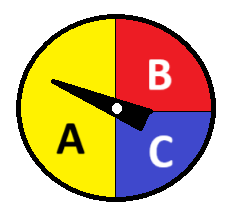
\includegraphics[width=0.2\linewidth]{figs/spinner.png}
\end{center}
\\~\\
You spin the spinner depicted above, and if it lands in the zone A, you win \$14; if it lands in the zone B, you win \$3; and if it lands in the zone C, you lose \$10. What is the expected amount of money you will win? 
\end{problem}
\medskip


\begin{problem}
Let $X$ be a random variable with the following PDF:
\[
f_X(x) = \begin{cases}
    (x-1)^3, & 1 \le x \le 3 \\
    0, & \text{otherwise}
\end{cases}
\]
Find the expectation and variance of $X$. 
\end{problem}


    % 
 \begin{center}\begin{large} Final Test\\
\textarmenian{Եզրափակիչ թեստ}
 \vspace{1em}
 
 \end{large}\end{center}
 \small Each question is worth one point. Duration: 150 minutes.\\
\textarmenian{Յուրաքանչյուր հարց գնահատվում է մեկ միավոր։ Տևողությունը՝ 150 րոպե։}
 \bigskip

 
\begin{problem}
Find the value of the expression:
\[ (3\va+4\vb)\cdot (\va-2\vc), \]
where
$\va=[2, 3, 2]^T,\,\vb=[0, -3, 2]^T,\,\vc=[-2, 5, -1]^T$.
\\
\textarmenian{Գտնել արտահայտության արժեքը, որտեղ $\va, \vb, \vc$ վեկտորները տրված վեկտորներն են։}
\end{problem}
\medskip

\begin{problem}
Calculate the L1 (Manhattan) and L2 (Euclidean) norms of the following vector:
\[ \dfrac{1}{3}\va+\dfrac{2}{3}\vb, \]
where $\va=[-5,4,10]^T,\,\vb=[1,0,7]^T$.
\\
\textarmenian{Հաշվել տրված վեկտորների {\rm L1} (մանհեթընյան) և {\rm L2} (էվկլիդեսյան) նորմերը։}
\end{problem}
\medskip

\begin{problem}
Find the angle between $\va$ and $\vb$ in the previous problem.
\\
\textarmenian{Գտնել նախորդ խնդրի $\va$ և $\vb$ վեկտորների կազմած անկյունը։}
\end{problem}
\medskip

\begin{problem}
Find the dimension of $\operatorname{span}\{\vv_1,\vv_2,\vv_3\}$ if
\[
\vv_1 = \begin{bmatrix}
    7 \\ 2 \\ 5
\end{bmatrix},
\qquad
\vv_2 = \begin{bmatrix}
    4 \\ 4 \\ 14
\end{bmatrix},
\qquad
\vv_3 = \begin{bmatrix}
    -11 \\ 4 \\ 20
\end{bmatrix}.
\]
\\
\textarmenian{Գտնել $\operatorname{span}\{\vv_1,\vv_2,\vv_3\}$-ի չափողականությունը։}
\end{problem}
\medskip

\begin{problem}
Given the matrices
\[ A = \begin{bmatrix}
-1&0&0&-2\\1&0&5&-5\\0&1&4&0\\0&0&-5&0
\end{bmatrix},\qquad B = \begin{bmatrix}
4&3&4&2\\8&7&5&3\\4&3&8&5\\4&3&4&3
\end{bmatrix}, \]
find $\det(AB)$.
\\
\textarmenian{Տրված մատրիցների համար գտնել $\det(AB)$-ն։}
\end{problem}
\medskip

\begin{problem}
Solve the SLE:
\[
\begin{cases}
    4x - y + 3z = 2\\
    11x + 4y - 9z = 11\\
    x + 2y - 5z = 3
\end{cases}
 \]
\\
\textarmenian{Լուծել գծային հավասարումների համակարգը (Գ\-ՀՀ)։}
\end{problem}
\medskip


\begin{problem}
Check if the matrix is positive definite:
\[ A = \begin{bmatrix}
2& -1& 0& 3\\
-1& 2 &-1 & 2\\
0& -1& 2 & 1 \\
-4& -2& -4 & 3 
\end{bmatrix}.\]
\\
\textarmenian{Ստուգել՝ արդյո՞ք մատրիցը դրական որոշյալ է։}
\end{problem}
\medskip

\begin{problem}
Find the algebraic and geometric multiplicities of the eigenvalues of the following matrix:
\[ A = \begin{bmatrix}
7 &0& -3\\
-9 &-2& 3\\
18 &0& -8
\end{bmatrix}. \]
\\
\textarmenian{Գտնել մատրիցի սեփական արժեքների հանրահաշվական և երկրաչափական պատիկությունները։}
\end{problem}
\medskip


\begin{problem}
Find the points of local extrema of the following function:
\[ f(x) = x^{2}+\ln\left(x+3\right), \]
and check if they are minimum or maximum points.
\\
\textarmenian{Գտնել ֆունկցիայի լոկալ էքստրեմումի կետերը և ստուգել՝ մինիմումի կետեր են, թե մաքսիմումի։}
\end{problem}
\medskip



\begin{problem}
Find the area under the graph of the following function between the lines $x=0$ and $x=2$:
\[ f(x) = x^{2}+\frac{\sin\left(\pi x\right)}{\pi} \]
\\
\textarmenian{Գտնել հետևյալ ֆունկցիայի գրաֆիկի տակի մակերեսը $x=0$ և $x=2$ ուղիղների միջև։}
\end{problem}
\medskip



\begin{problem}
Compute the gradient of the function:
\[ f(x,y,z) = \dfrac{3x^2e^{1-z^2}}{y} \]
at the point $(-2,3,1)$.
\\
\textarmenian{Հաշվել ֆունկցիայի գրադիենտը $(-2,3,1)$ կետում։}
\end{problem}
\medskip



\begin{problem}
Compute the directional derivative of the function:
\[ f(x,y) = x^2 + 2xy - y^2 \]
in the direction of $[0.6,\;0.8]^T$ at the point $(1, 1)$.
\\
\textarmenian{Գտնել $[0.6,\;0.8]^T$ վեկտորի ուղղությամբ ֆունկցիայի ածանցյալը $(1, 1)$ կետում։}
\end{problem}
\medskip

\begin{problem}
Find the points of local extrema of the following function:
\[f(x, y) = x^4 - 4x^2 + y^2\]
Check if they are minimum or maximum points.
\\
\textarmenian{Գտնել ֆունկցիայի լոկալ էքստրեմումի կետերը և ստուգել՝ մինիմումի կետեր են, թե մաքսիմումի։}
\end{problem}
\medskip



\begin{problem}
Two fair dice are rolled. What is the probability of getting $4$ on exactly one of them, given that their sum is even?
\\
\textarmenian{Նետել ենք երկու իսկական զառ։ Որքա՞ն է հավանականությունը, որ դրանցից ուղիղ մեկն ընկել է $4$, եթե հայտնի է, որ ընկած թվերի գումարը զույգ է։}
\end{problem}
\medskip


\begin{problem}
There are $9$ books on a bookshelf, $3$ on culinary, $6$ on arts. Hakob randomly takes three of them. What is the probability that all of those three are on the same subject?
\\
\textarmenian{Գրապահարանին կա $9$ գիրք՝ $3$-ը խոհարարության մասին, $6$-ը՝ արվեստի։ Հակոբը պատահականորեն վերցնում է դրանցից երեքը։ Որքա՞ն է հավանականությունը, որ երեքն էլ կլինեն նույն թեմայի շուրջ։}
\end{problem}
\medskip

\begin{problem}
The first album contains twice as much songs than the second. Moreover, $20\%$ of songs in the first album are in Armenian, while in the second album $45\%$ are. The DJ plays a random song in Armenian. What is the probability that the song was from the first album?
\\
\textarmenian{Առաջին ալբոմում կա երկու անգամ ավելի շատ երգ, քան երկրորդում։ Ընդ որում, առաջին ալբոմի երգերի $20\%$-ն են հայերեն, իսկ երկրորդ ալբոմի՝ $45\%$-ը։ {\rm DJ}-ը պատահականորեն դնում է որևէ հայերեն երգ։ Որքա՞ն է հավանականությունը, որ դրված երգն առաջին ալբոմից է։}
\end{problem}
\medskip


\begin{problem}
We toss a coin, and if it's heads we win \$2. Otherwise, we toss it once more, and if it's heads we win \$1, if it's tails, we win \$3. What is the probability of winning more than \$1 in this game?
\\
\textarmenian{Նետում ենք մետաղադրամը, և եթե ընկնում է գիր, շահում ենք \$2։ Հակառակ դեպքում՝ նետում ենք ևս մեկ անգամ, և եթե ընկնում է գիր, շահում ենք \$1, եթե ղուշ՝ շահում ենք \$3։ Որքա՞ն այս խաղում \$1-ից ավելի շահելու հավանականությունը։}
\end{problem}
\medskip



\begin{problem}
Anna and Ani plan to meet each other somewhere between 19:00 and 20:00. If Ani arrives sooner than Anna, she waits for another $10$ minutes, and if Anna doesn't come, she leaves. If Anna arrives sooner than Ani, she waits for $5$ minutes, and if Ani doesn't come, she leaves. What is the probability that they will meet if both of them arrive at some random time between 19:00 and 20:00?
\\
\textarmenian{Աննան և Անին պլանավորում են հանդիպել 19:00-20:00 միջակայքում ինչ-որ պահի։ Եթե Անին Աննայից շուտ է հասնում, նա սպասում է ևս $10$ րոպե և, եթե Աննան չի գալիս, հեռանում։ Եթե Աննան Անիից շուտ է հասնում, նա սպասում է ևս $5$ րոպե և, եթե Անին չի գալիս, հեռանում։ Որքա՞ն է հավանականությունը, որ նրանք կհանդիպեն, եթե երկուսն էլ տեղ են հասնում 19:00-ի և 20:00-ի միջև որևէ պատահական պահի։}
\end{problem}
\medskip

\begin{problem}
% \\~\\
\begin{center}
    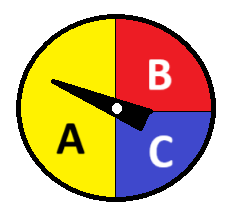
\includegraphics[width=0.2\linewidth]{figs/spinner.png}
\end{center}
% \\~\\
You spin the spinner depicted above, and if it lands in the zone A, you win \$14; if it lands in the zone B, you win \$3; and if it lands in the zone C, you lose \$10. What is the expected amount of money you will win? 
\\
\textarmenian{Դուք պտտում եք վերևում պատկերված պտուտակը, և եթե սլաքը հայտնվում է {\rm A} գոտում, ապա հաղթում եք \$14, եթե հայտնվում է {\rm B} գոտում, հաղթում եք \$3, իսկ եթե հայտնվում է {\rm C} գոտում, պարտվում եք \$10: Որքա՞ն է շահելիք գումարի սպասվող չափը (մաթսպասումը)։}
\end{problem}
\medskip


\begin{problem}
Let $X$ be a random variable with the following PDF:
\[
f_X(x) = \begin{cases}
    (x-1)^3, & 1 \le x \le 3 \\
    0, & \text{otherwise}/\textarmenian{հակառակ դեպքում}
\end{cases}
\]
Find the expectation and variance of $X$. 
\\
\textarmenian{Դիցուք $X$-ը տրված խտության ֆունկցիայով պատահական մեծություն է։ Գտնել $X$-ի մաթսպասումը և վարիացիան։}
\end{problem}


    
    
    
    %  \begin{center}\begin{large} Sample Test
 \vspace{1em}
 
 \end{large}\end{center}
 \small Each question is worth 100/15 points. Duration: 115 minutes.
 \bigskip

 
\begin{problem}
Find the value of the expression:
\[ (6\va+5\vb)\cdot (\va-2\vc), \]
where $\va=[1, 3, 2]^T,\,\vb=[0, -3, 5]^T,\,\vc=[1, 5, 1]^T$.
\end{problem}
\medskip

\begin{problem}
Calculate the L1 (Manhattan) and L2 (Euclidean) norms of the following vector:
\[ \dfrac{1}{4}\va-\vb, \]
where $\va=[7,4,1]^T,\,\vb=[1,0,3]^T$.
\end{problem}

\medskip

\begin{problem}
Given the matrices
\[ A = \begin{bmatrix}
7& 2 &4 &0\\
1 &5 &0 &0\\
4 &2 &0& 1\\
−2 &3 &1 &2
\end{bmatrix},\qquad B = \begin{bmatrix}
2 &1 &5&0\\
0 &3& 0&2\\
7 &6 &-1&2\\
2&0&1&4
\end{bmatrix}, \]
find $\det(AB)$.
\end{problem}
\medskip



\begin{problem}
Solve the SLE:
\[
\begin{cases}
    2x+y+z = 2\\
    x - 4y - 9z = 11\\
    4x + 2y - 5z = 4
\end{cases}
 \]
\end{problem}
\medskip


\begin{problem}
Check if the matrix is positive definite:
\[ A = \begin{bmatrix}
2& -1& 4\\
-1& 6 &0\\
4& 0& 2
\end{bmatrix}.\]
\end{problem}
\medskip

\begin{problem}
Find the eigenvalues and eigenvectors of the following matrix:
\[ A = \begin{bmatrix}
1&2&3\\3&2&1\\2&1&3
\end{bmatrix}. \]
\end{problem}
\medskip


\begin{problem}
Find the points of local extrema of the following function:
\[ f(x) =3x^2-x^5\]
on $x\in [-2,2]$. Check if they are minimum or maximum points.
\end{problem}
\medskip



\begin{problem}
Find the area under the graph of the following function between the lines $x=0$ and $x=1$:
\[ f(x) =5x^{\frac{3}{2}}+e^{x-3}\]
\end{problem}
\medskip



\begin{problem}
Compute the gradient of the function:
\[ f(x,y,z) = \dfrac{y^3\cos{yz}}{\sqrt{x}} \]
at the point $(2,3,0)$.
\end{problem}
\medskip



\begin{problem}
Compute the directional derivative of the function:
\[ f(x,y) = x^3 - xy^2 \]
in the direction of ${1\over\sqrt{5}} [1,2]^T$ at the point $(2, 4)$.
\end{problem}
\medskip

\begin{problem}
Find the points of local extrema of the following function:
\[f(x, y) = x^3 - 2x^2 - y^2\]
Check if they are minimum or maximum points.
\end{problem}
\medskip



\begin{problem}
Two fair dice are rolled. What is the probability of getting $5$ on at least one of them, given that their sum is odd?
\end{problem}
\medskip


\begin{problem}
There are $10$ red, $7$ blue balls in a box. We randomly take three of them. What is the probability that there are both red and blue balls among them?
\end{problem}
\medskip

\begin{problem}
The supermarket sells 4 times more tablecloths than the shop, but only half of them are green, while $80\%$ of the tablecloths sold by the shop are green. If a randomly selected tablecloth is green, what is the probability that it was bought from the shop?
\end{problem}
\medskip


\begin{problem}
Khachik thinks of a whole number (integer) and asks Vachik to keep another whole number in his mind. If Vachik's number is greater than that of Khachik, Vachik wins, otherwise Khachik wins. We know that if Khachik loses, he will ask for another round and they will play one more time. What is the probability that after all, Khachik would win at least once?
\end{problem}
\medskip
    %  \begin{center}\begin{large} Final Test
 \vspace{1em}
 
 \end{large}\end{center}
 % \small Each question is worth 100/15 points. Duration: 115 minutes.
 \bigskip


\begin{problem} \textbf{True/False Questions:}

\begin{enumerate}
    % \item Regularization techniques are used to prevent overfitting in machine learning models.

    % \item Hyperparameters are parameters that are set prior to the training process and are not learned from the data.

    % \item K-medoids is a supervised learning algorithm.

%     \item Missing data should always be \textit{removed} from the dataset to prevent any negative impact
% on model performance

%     \item Classification is used when the target variable is categorical, while regression is used
% when the target variable is continuous.
    
%     \item Overfitting occurs when a model performs well on both the training and testing.

% True or False: PCA can be used for feature extraction as well as dimensionality reduction.

    % \item The random forest algorithm is an example of an unsupervised learning technique.



    \item In general, having a deeper  decision tree is better than a shallower one.

    \item In hierarchical clustering, the choice of linkage method determines how clusters are formed.

    % \item The K-Nearest Neighbors algorithm requires training time but no prediction time.

    \item The purpose of regularization is to penalize large coefficients in a model.


    % \item PCA (Principal Component Analysis) can be used for dimensionality reduction in a dataset.
\end{enumerate}
    
\end{problem} 

% True or False: Ensemble methods combine multiple machine learning models to improve performance.


\begin{problem} \textbf{Multiple-Choice Question:}

\item Which criteria are used for splitting nodes in decision trees? Choose all that apply.


\begin{enumerate}
    \item [a)] Mean Squared Error (MSE)
    \item [b)] Gini impurity
    \item [c)] Variance
    \item [d)] Entropy
\end{enumerate}
% 
% a) 
% b) 
% d) 
\end{problem}


\begin{problem} \textbf{Short Answer Questions:}

\begin{enumerate}
    % \item What is feature engineering, and why is it important in machine learning?

    \item 
What is the purpose of having separate Train, Validation, Test datasets?


    \item 
 What is the learning rate in gradient descent optimization algorithms, why do we need it?


\end{enumerate}
    
\end{problem}




\begin{problem}
    \textbf{Linear Regression:}



\begin{itemize}
    \item Describe how the Ordinary Least Squares (OLS) algorithm works
    
    \item Why may large weights be unwanted?

    \item What are some techniques to prevent large weights?
\end{itemize}
\end{problem}

% Multiple-Choice Questions:

% Which evaluation metric is most appropriate for imbalanced datasets?
% a) Accuracy
% b) Precision
% c) F1-score
% d) Mean Squared Error (MSE)

% Explain the bias-variance tradeoff in machine learning.
% Describe the curse of dimensionality and its implications in machine learning.

% Explain the concept of bias in machine learning models and how it can affect model performance.
% What is the difference between batch gradient descent, stochastic gradient descent, and mini-batch gradient descent?



% True or False: PCA is a supervised learning algorithm.
% True or False: Support Vector Machines are primarily used for regression tasks.


% Short Answer Questions:

% What is the purpose of a learning rate in gradient descent optimization algorithms?

% Multiple-Choice Questions:

% Which of the following algorithms is a non-parametric method?
% a) Linear Regression
% b) Decision Trees
% c) Logistic Regression
% d) Ridge Regression


% 1. True/False Questions.
% [1.1] Supervised learning requires labeled training data, while unsupervised learning
% can work with unlabeled data.
% # True # False
% [1.2] Classification is used when the target variable is categorical, while regression is
% used when the target variable is continuous.
% # True # False
% [1.3] Overfitting occurs when a model performs well on both the training and testing
% data.
% # True # False
% [1.4] Missing data should always be removed from the dataset to prevent any negative
% impact on model performance.
% # True # False
% [1.5] Feature scaling is a preprocessing technique used to bring all features to the
% range between 0 and 1.
% # True # False

% 2. Multiple-Choice Questions.
% [2.1] Ordinary Least Squares (OLS) is used in linear regression to minimize:
% # Mean Squared Error
% # Mean Absolute Error
% [2.2] Gradient descent is an optimization algorithm used to::
% # Find the maximum of a function.
% # Minimize the loss function and find optimal parameters.
% # Randomly initialize model weights.
% 2
% [2.3] Which type(s) of gradient descent doesn’t use the entire dataset in each iteration?
% Choose all that apply.
% # Batch gradient descent
% # Stochastic gradient descent
% # Mini-batch gradient descent
% [2.4] Which of the following are possible metrics used to evaluate linear regression
% models? Choose all that apply.
% # Mean Absolute Error (MAE)
% # Precision
% # Accuracy
% # Root Mean Squared Error (RMSE)
% [2.5] Which of the following are components of the logistic regression algorithm?
% Choose all that apply.
% # Sigmoid function
% # Mean Absolute Error (MAE)
% # Cross-entropy loss function
% # Root Mean Squared Error (RMSE)
% [2.6] What does the confusion matrix provide insights into?
% # Precision and Recall
% # Feature importance
% # Mean squared error
% # Bias-variance tradeoff
% [2.7] Which criterias are used for splitting nodes in decision trees? Choose all that
% apply.
% # Mean Squared Error (MSE)
% # Gini impurity
% # Variance
% # Entropy
% [2.8] Which of the following are examples of ensemble methods? Choose all that apply.
% # Random Forest
% # Logistic Regression
% # Gradient Boosting
% # K-Means
% 3
% 3. Gradient Descent
% You are using gradient descent to find the minimum of the function
% f(x) = x
% 2
% You experiment by fixing the number of iterations and trying different learning rates
% to find the one which leads to a better (smaller) solution. There are different possible
% settings, e.g., you choose a learning rate of zero (1), the optimal learning rate (2), a
% learning rate that is too large (3) or too small (4). When initializing at point A on the
% plot below, which point of the plot are you most likely to reach with each learning rate
% setting? Match the settings 1, 2, 3, and 4 to the points on the plot indicated by letters
% A,B, C, and D.
% 4. Logistic Regression
% [4.1] Arrange the steps of the logistic regression algorithm in the correct order:
% • A. Compute the weighted sum of inputs and weights.
% • B. Calculate the loss using the binary cross-entropy function.
% • C. Update the weights using gradient descent.
% • D. Apply the sigmoid function to the weighted sum.
% [4.2] Write the formula of sigmoid function.
% 4
% 5. Bias-Variance Decomposition
% Examine the provided graph illustrating the bias-variance tradeoff based on model
% complexity. In which region of the graph does the model overfit the data? Where does
% the model underfit the data? Finally, identify the area on the graph that represents the
% optimal balance between bias and variance. Use the terms ’overfitting,’ ’underfitting,’
% and ’optimal solution’ to describe each respective region.
% 6. KNN
% Describe how the K-Nearest Neighbors (KNN) algorithm works (prediction
% stage)
% • Given a new input data point for classification or regression.
% • Identify the value of k, which represents the number of nearest neighbors to consider.
% • ....
% 5
% 7. Confusion Matrix
% You are given a set of actual labels and the probability outputs as predictions from a
% binary classification model.
% Actual Label Probability Output Prediction 1 Prediction 2
% 1 0.75
% 0 0.42
% 1 0.63
% 1 0.82
% 0 0.28
% 1 0.91
% 0 0.35
% 1 0.76
% 0 0.19
% 0 0.67
% 1. Choose two threshold values and find predictions.
% 2. For each prediction construct a confusion matrix using the provided actual labels
% and probability outputs.
% 3. Calculate the precision and recall values based on the confusion matrices.
% 6
% 7. Decision Tree
% You are provided with an image depicting a decision tree applied to 2D data. Your
% task is to construct a decision tree based on the given image that captures the same
% structure and decisions as shown in the picture.
    % \begin{center}\begin{large} Final Test
 \vspace{1em}
 
 \end{large}\end{center}
 % \small Each question is worth 100/15 points. Duration: 115 minutes.
 \bigskip


\begin{problem} \textbf{True/False Questions:}

\begin{enumerate}
 
    \item A decision tree can handle both numerical and categorical data.

    \item In hierarchical clustering, the choice of linkage method determines how clusters are formed.

    \item The purpose of regularization is to penalize large coefficients in a model.

    % \item The K-Nearest Neighbors algorithm requires training time but no prediction time.

\end{enumerate}
    
\end{problem} 



\begin{problem} \textbf{Multiple-Choice Question:}

\item Which criteria are used for splitting nodes in decision trees? Choose all that apply.

\begin{enumerate}
    \item [a)] Mean Squared Error (MSE)
    \item [b)] Gini impurity
    \item [c)] Variance
    \item [d)] Entropy
\end{enumerate}

\end{problem}


\begin{problem} \textbf{Short Answer Questions:}

\begin{enumerate}
    % \item What is the purpose of the bias in a neural network?
    
    \item Write the formula of ReLU function. What is it suitable for?

    \item 
Describe the difference between K-Means and K-Medoids.

    \item 
What is the purpose of having separate Train, Validation, Test datasets?

\end{enumerate}
    
\end{problem}




\begin{problem}
    \textbf{Linear Regression:}

\begin{itemize}
    \item Describe how the Ordinary Least Squares (OLS) algorithm works.
    
    \item Why may large weights be unwanted?

    \item What are some techniques to prevent large weights?
\end{itemize}
\end{problem}


    % 

\begin{problem}

    \begin{enumerate}

\item[a.] Implement the following optimizers:
\begin{itemize}
   % \item Stochastic Gradient Descent
    \item RMSProp
    \item \textbf{(optional)} Adagrad
  %  \item Adam
\end{itemize}


\item[b.] Construct a Fully Connected network and use the optimizers implemented in \textbf{a)}, as well as Adam and SGD from PyTorch to train the network on the following regression {\color{blue}\href{https://scikit-learn.org/stable/modules/generated/sklearn.datasets.fetch_california_housing.html}{dataset}}.

\item[c.] Experiment with different initialization methods and compare the results. You may want to use \verb|torch.nn.init|.
    \end{enumerate}
\end{problem}
    

\end{document}